\documentclass[12pt]{article}
\usepackage[utf8]{inputenc}
\usepackage[T1]{fontenc}
\usepackage[english]{babel}
\usepackage{tabularx}
\usepackage{float} % Pacchetto per l'opzione di posizionamento H
\usepackage{caption} % Pacchetto per gestire le didascalie delle figure
\usepackage{subcaption}
\usepackage{url}
\usepackage{geometry}
\usepackage{graphicx}
\usepackage[hyperfootnotes=false]{hyperref} % Riferimenti
\usepackage{setspace} %interlinea
\usepackage{pdfpages}
\usepackage{pdflscape}
\usepackage{verbatim}
\usepackage{afterpage}
\usepackage{booktabs}
\usepackage{amsmath}
\usepackage{bm}

\usepackage{enumitem}
\usepackage{xcolor}
\usepackage{listings}

% Code listings -------------------------------------------------------------
\definecolor{lstBg}{HTML}{F9FAFB}
\definecolor{lstRule}{HTML}{E5E5E5}
\definecolor{lstComment}{HTML}{6B7280}
\definecolor{lstKeyword}{HTML}{B4413F}
\definecolor{lstString}{HTML}{2F6F4E}

\lstdefinelanguage{JavaScript}{
  keywords={await, async, break, case, catch, const, continue, default, delete,
            do, else, export, extends, false, finally, for, from, function, if,
            import, in, instanceof, let, new, null, of, return, super, switch,
            this, throw, true, try, typeof, undefined, var, void, while, yield},
  sensitive=true,
  comment=[l]{//},
  morecomment=[s]{/*}{*/},
  morestring=[b]',
  morestring=[b]",
  morestring=[b]`,
}

\lstset{
  basicstyle=\ttfamily\footnotesize,
  backgroundcolor=\color{lstBg},
  frame=single,
  rulecolor=\color{lstRule},
  framesep=6pt,
  keywordstyle=\color{lstKeyword},
  commentstyle=\color{lstComment}\itshape,
  stringstyle=\color{lstString},
  columns=fullflexible,
  keepspaces=true,
  showstringspaces=false,
  upquote=true,
  breaklines=true,
  breakatwhitespace=true,
  captionpos=b,
  abovecaptionskip=6pt,
  aboveskip=12pt,
  belowskip=12pt,
  xleftmargin=6pt,
  xrightmargin=6pt,
}
\renewcommand{\lstlistingname}{Listing}

\onehalfspacing

\begin{document}

% FRONTESPIZIO
\hypersetup{pageanchor=false}

\includepdf{docs/frontespizioMAD.pdf}
\hypersetup{pageanchor=true}

\renewcommand{\contentsname}{Summary}
\pagenumbering{Roman}
\tableofcontents
\newpage
\listoffigures
\newpage
\listoftables

% RICHIAMO CAPITOLI
\newpage
\pagenumbering{arabic}

\section{Introduction}\label{sect:Introduction}
This report documents the design and development process of TrainHub, a Progressive Web App (PWA) created for the Mobile Application Development course. TrainHub is an all-in-one digital platform designed specifically for physical gyms, aiming to seamlessly connect gym members with the facility's certified professionals, such as Personal Trainers (PTs), nutritionists, and dietitians.

The fitness industry often suffers from severe digital fragmentation. Users are frequently forced to navigate between disparate applications to track their workouts, log their meals, book appointments, and communicate with their trainers. TrainHub was born from the necessity to solve this "app fatigue" by centralizing the entire fitness journey into a single, cohesive environment.

\subsection{Preliminary Features}\label{subsect:PreliminaryFeatures}
Before diving into the user research and market analysis, we defined a preliminary set of core functionalities to guide the initial scope of our project. These essential features aim to cover the fundamental needs of both modern gym-goers and fitness professionals:

\begin{itemize}
    \item \textbf{Personalized Workout Tracking:} a comprehensive module allowing users to log their daily exercises and monitor their progress. These routines can be independently created by the user or professionally designed and assigned by a Personal Trainer (e.g., if the client has purchased a customized training protocol);
    \item \textbf{Diet and Nutrition Management:} a dedicated section for dietary planning. To ensure safety and reliability, diet plans can exclusively be created and updated by certified professionals, while users can view them and track their daily adherence;
    \item \textbf{Appointment and Service Booking:} an integrated calendar system enabling users to easily book consultations with nutritionists/dietitians, reserve one-on-one training sessions with PTs, or manage their gym schedule;
    \item \textbf{Digital Facility Access:} a built-in digital membership card (e.g., via QR code) that simplifies the user's physical entry into the gym, eliminating the need for traditional plastic badges and speeding up the check-in process.
\end{itemize}

\subsection{Target Users}\label{subsect:TargetUsers}
Given the platform's dual nature, serving both the demand and supply sides of the gym ecosystem, we identified two distinct categories of potential users, each requiring a tailored interface and specific system privileges:

\begin{itemize}
    \item \textbf{Gym Members (Clients):} the primary end-users of the application. They utilize TrainHub to track their fitness progress, consult their assigned diets, book appointments, and interact directly with their trainers. Their interface prioritizes ease of use, fast data entry during workouts, and clear visualization;
    \item \textbf{Gym Professionals (Admins):} the staff members working within the facility, including Personal Trainers, Nutritionists, and Dietitians. This user group requires an "Admin" profile with advanced privileges. They use the platform as a management tool to monitor their clients' progress, create and distribute workout/diet plans, manage their booking schedules, and maintain direct communication with the members.
\end{itemize}

By addressing the specific needs of both user groups within a single PWA, TrainHub strives to enhance the overall customer experience while simultaneously optimizing the daily workflow of gym professionals.
\newpage
\section{Competitors Analysis}\label{sect:CompetitorsAnalysis}In this chapter, we present the Competitor Analysis, which is a fundamental step in the design process of TrainHub. Before developing our application, we researched the current market to understand how other companies have tackled similar problems and to identify areas where our project could stand out.

To conduct this analysis, we searched the main mobile stores (Google Play Store and Apple App Store) for apps related to fitness and gym management. We selected a few key applications, downloaded them, and tested their main functionalities.

For comparison purposes, we divided the analyzed applications into two main categories:
\begin{itemize}
    \item \textbf{Direct Competitors: }applications that try to solve the same problem, with the same value proposition, for the same target users;
    \item \textbf{Indirect Competitors: }applications that target a similar user group but with a different value proposition, or vice versa.
\end{itemize}

Overall, this study allowed us to identify the strengths and weaknesses of the current solutions on the market. By understanding what is already available, we were able to define the core features of TrainHub and highlight how our app can solve problems that others currently ignore.
\subsection{Direct Competitors}\label{subsect:DirectCompetitors}
For TrainHub, direct competitors are applications that are strictly tied to a physical gym environment. These apps aim to provide an all-in-one ecosystem that connects gym members with the facility and its professionals. Their main goal is to centralize the user's gym experience, offering tools such as digital access, course bookings, and training programs within a single platform.

Based on our market research, we identified four key players in this category. These include applications developed specifically for major gym chains, generalized management software widely used by local gyms, and global industry benchmarks that offer comprehensive business-to-business (B2B) and business-to-consumer (B2C) solutions.

To properly evaluate these competitors, we summarized our findings in the following two comparison tables:
\begin{itemize}
    \item \textbf{Dimensions Table:} this table compares general market aspects, such as the business model, pricing, and user ratings on digital stores, helping us understand the scale of these competitors;
    \item \textbf{Features Table:} this table breaks down the specific functionalities offered by each application.
\end{itemize}

By mapping out what these apps currently offer, we can clearly highlight the gaps in the market, such as the lack of fully integrated diet management and direct chat with professionals, and demonstrate how TrainHub can provide a more complete and seamless experience for both clients and gym staff.

\paragraph{Virgin Active}The Virgin Active app is the official mobile application for members of the Virgin Active gym chain. It provides an exclusive ecosystem that allows users to easily book classes, access remote training sessions, and stay updated on club news. Additionally, it offers practical tools to follow daily workouts, monitor personal performance, and track fitness progress in a centralized and interactive way.

\begin{figure}[H]
    \centering
    \begin{subfigure}{0.4\textwidth}
        \centering
        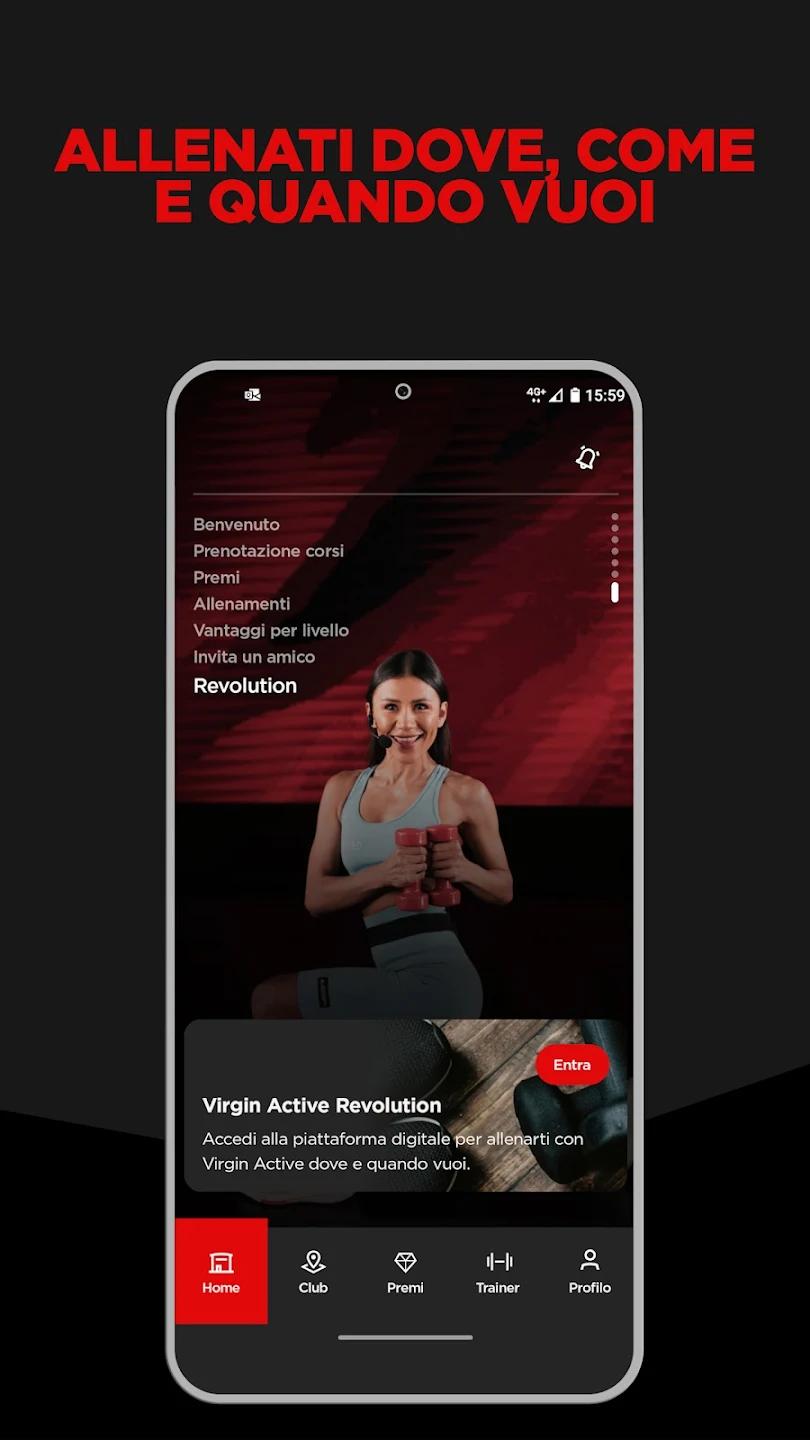
\includegraphics[width=\textwidth]{2-CompetitorsAnalysis/img/VirginActive/Home.jpg}
        \caption{Home Interface}
        \label{fig:virgin_home}
    \end{subfigure}
    % \hfill
    \begin{subfigure}{0.4\textwidth}
        \centering
        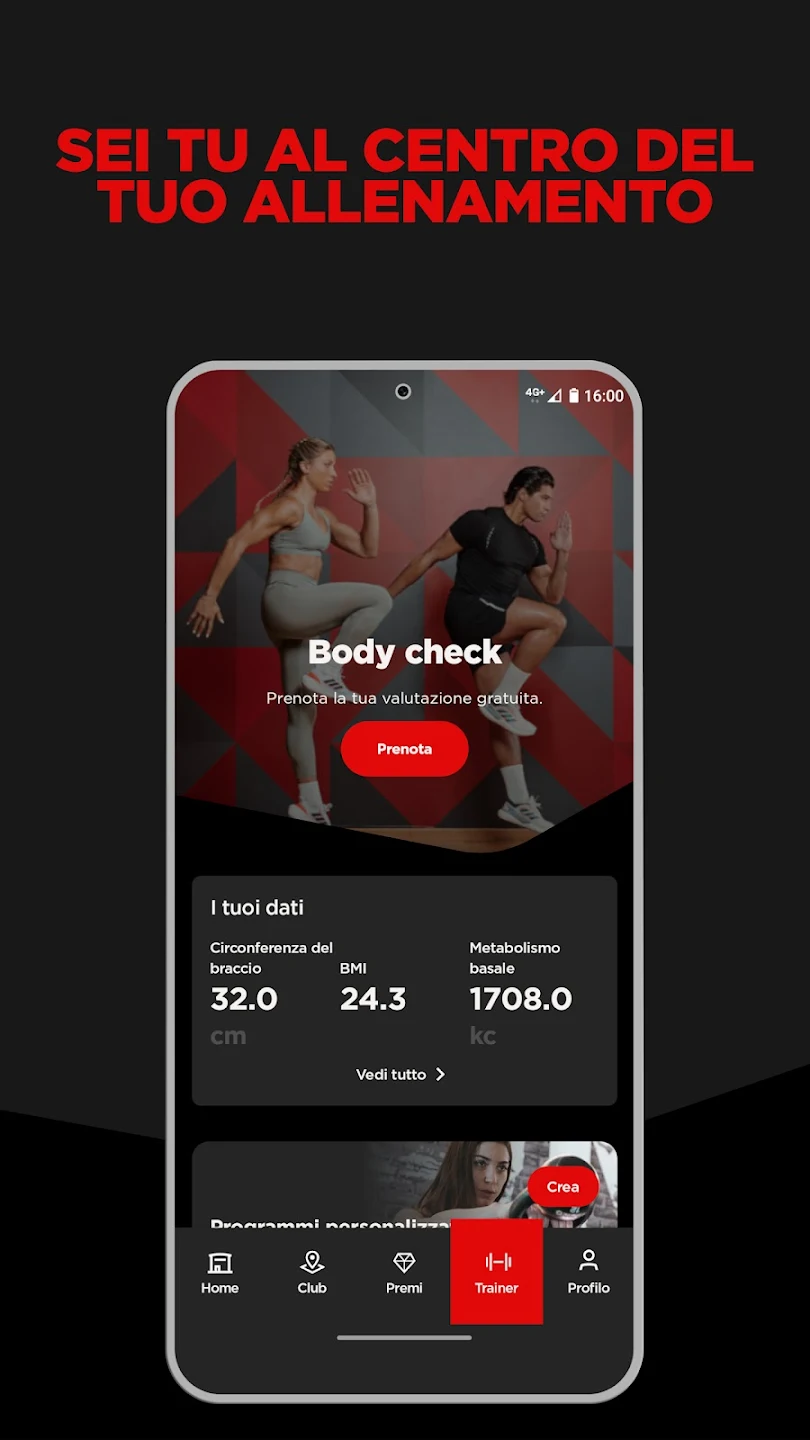
\includegraphics[width=\textwidth]{2-CompetitorsAnalysis/img/VirginActive/Trainer.jpg}
        \caption{Trainer Interface}
        \label{fig:virgin_trainer}
    \end{subfigure}
    \caption{Virgin Active App Interface}
    \label{fig:virgin_active_app}
\end{figure}

\paragraph{EvolutionFit Club}EvolutionFit is a comprehensive management application designed for both gym clients and personal trainers. It provides an all-in-one solution that integrates workout plan management, facility and class bookings, and detailed progress tracking. Furthermore, it features a dedicated nutrition section with a food diary and calorie goals, aiming to centralize the user's entire fitness and dietary journey into a single platform.

\begin{figure}[H]
    \centering
    \begin{subfigure}{0.4\textwidth}
        \centering
        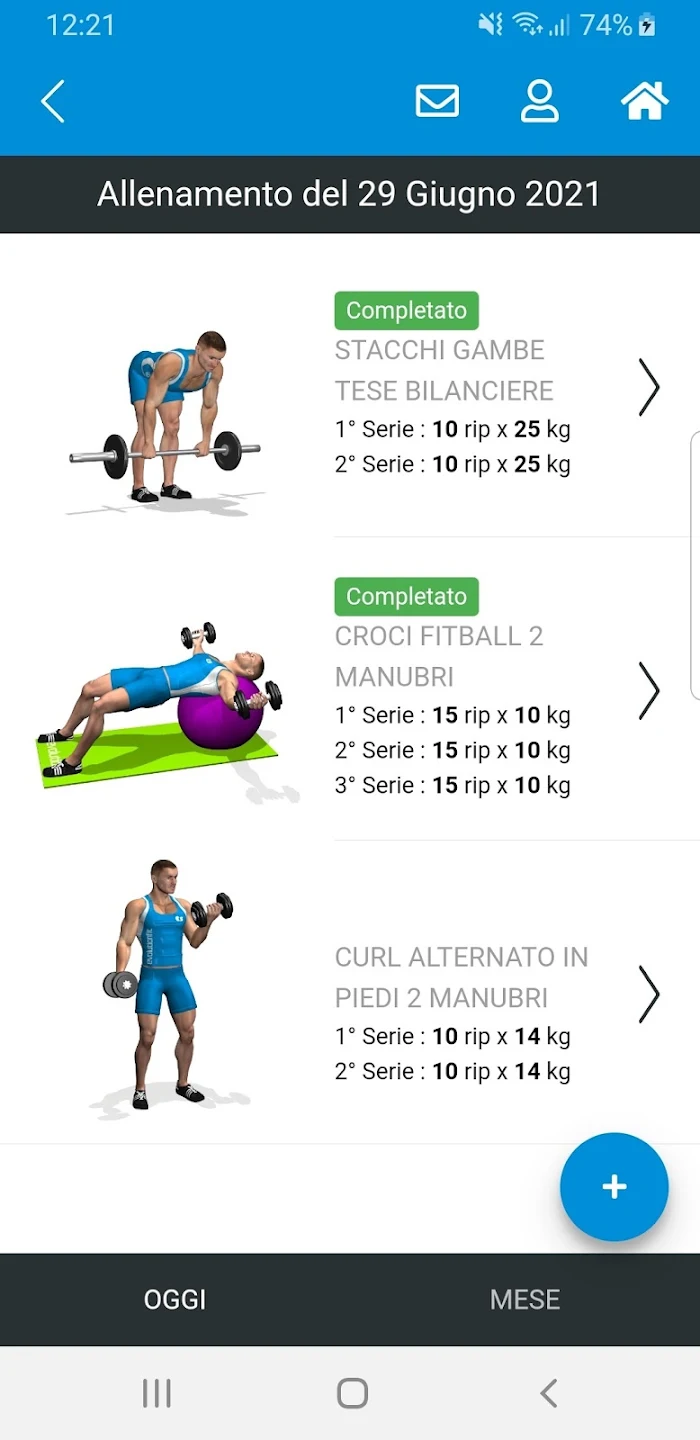
\includegraphics[width=\textwidth]{2-CompetitorsAnalysis/img/EvolutionFit/Workout.jpg}
        \caption{Workout Interface}
        \label{fig:evolution_workout}
    \end{subfigure}
    % \hfill
    \begin{subfigure}{0.4\textwidth}
        \centering
        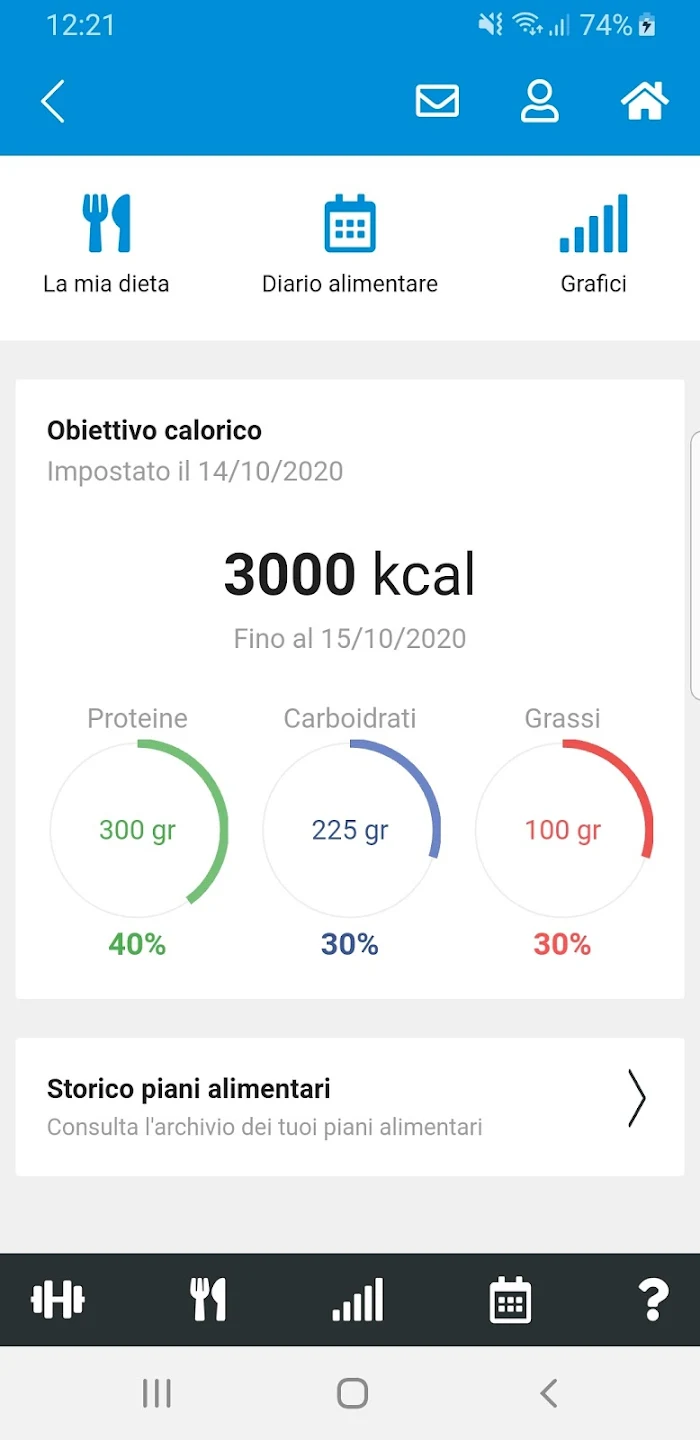
\includegraphics[width=\textwidth]{2-CompetitorsAnalysis/img/EvolutionFit/Nutrition.jpg}
        \caption{Nutrition Interface}
        \label{fig:evolution_nutrition}
    \end{subfigure}
    \caption{EvolutionFit App Interface}
    \label{fig:evolution_fit_app}
\end{figure}

\paragraph{Technogym}The Technogym App is a robust health and fitness platform powered by an AI Coach that generates customized training programs based on user goals, available time, and equipment. It features a vast library of over 1,000 on-demand workouts, holistic wellness content, and community challenges. The app also strongly focuses on performance monitoring by seamlessly syncing with major third-party wearables and health trackers.

\begin{figure}[H]
    \centering
    \begin{subfigure}{0.4\textwidth}
        \centering
        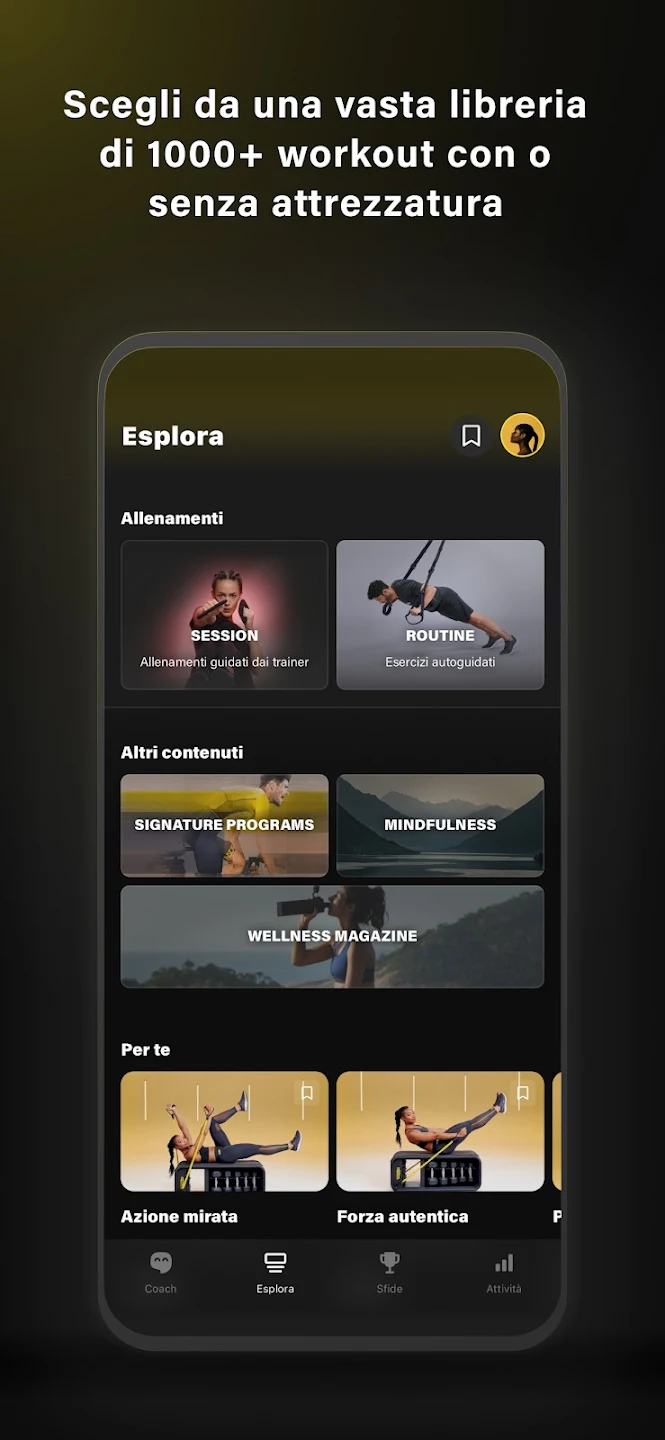
\includegraphics[width=\textwidth]{2-CompetitorsAnalysis/img/Technogym/Explore.jpg}
        \caption{Workout Interface}
        \label{fig:technogym_explore}
    \end{subfigure}
    % \hfill
    \begin{subfigure}{0.4\textwidth}
        \centering
        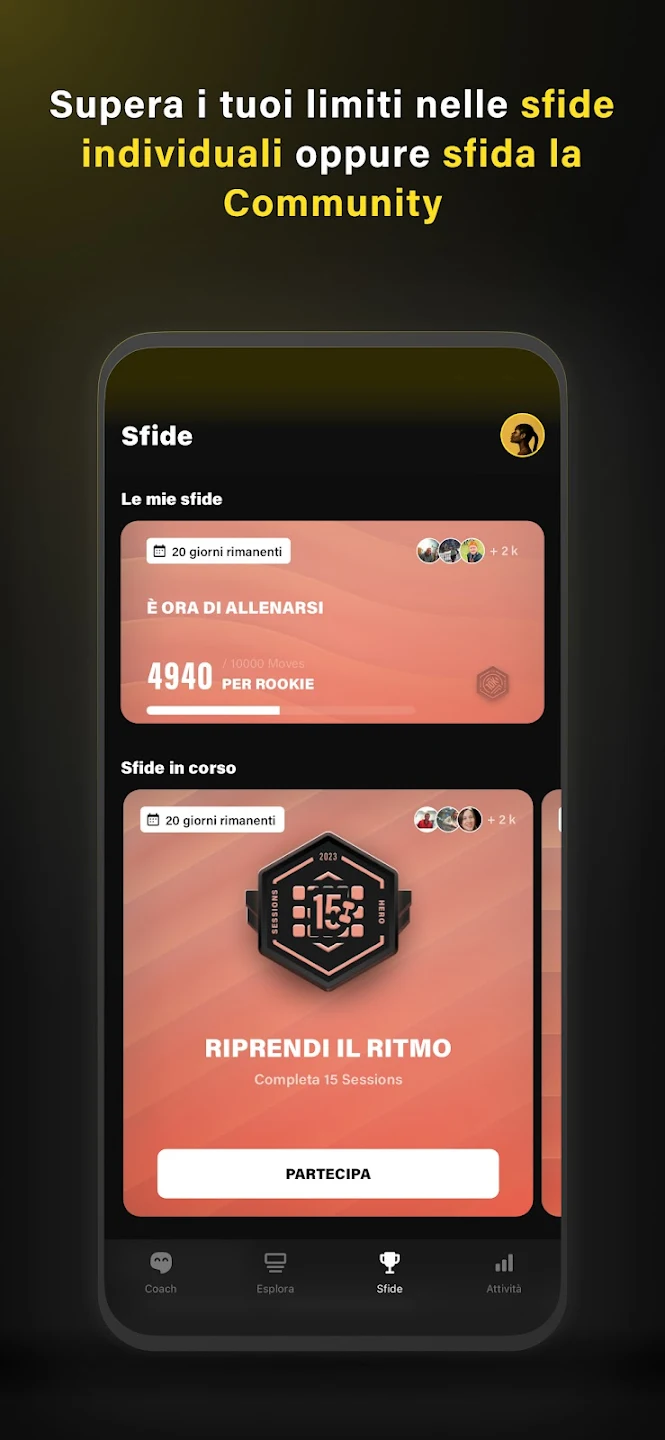
\includegraphics[width=\textwidth]{2-CompetitorsAnalysis/img/Technogym/Challenge.jpg}
        \caption{Challenge Interface}
        \label{fig:technogym_challenge}
    \end{subfigure}
    \caption{Technogym App Interface}
    \label{fig:technogym_app}
\end{figure}


\paragraph{Virtualgym}Virtuagym is a highly versatile fitness platform featuring an extensive database of over 4,000 exercises suitable for various fitness levels, locations, and equipment availability. A standout feature is its deep integration with its sister application, Virtuagym Food, which provides advanced macronutrient and calorie tracking. Together, they offer a complete ecosystem for both workout management and nutritional planning, supported by wearable integrations.

\begin{figure}[H]
    \centering
    \begin{subfigure}{0.4\textwidth}
        \centering
        
\includegraphics[width=\textwidth]{2-CompetitorsAnalysis/img/Virtualgym/Workout.jpg}
        \caption{Workout Interface}
        \label{fig:virtualgym_workout}
    \end{subfigure}
    % \hfill
    \begin{subfigure}{0.4\textwidth}
        \centering
        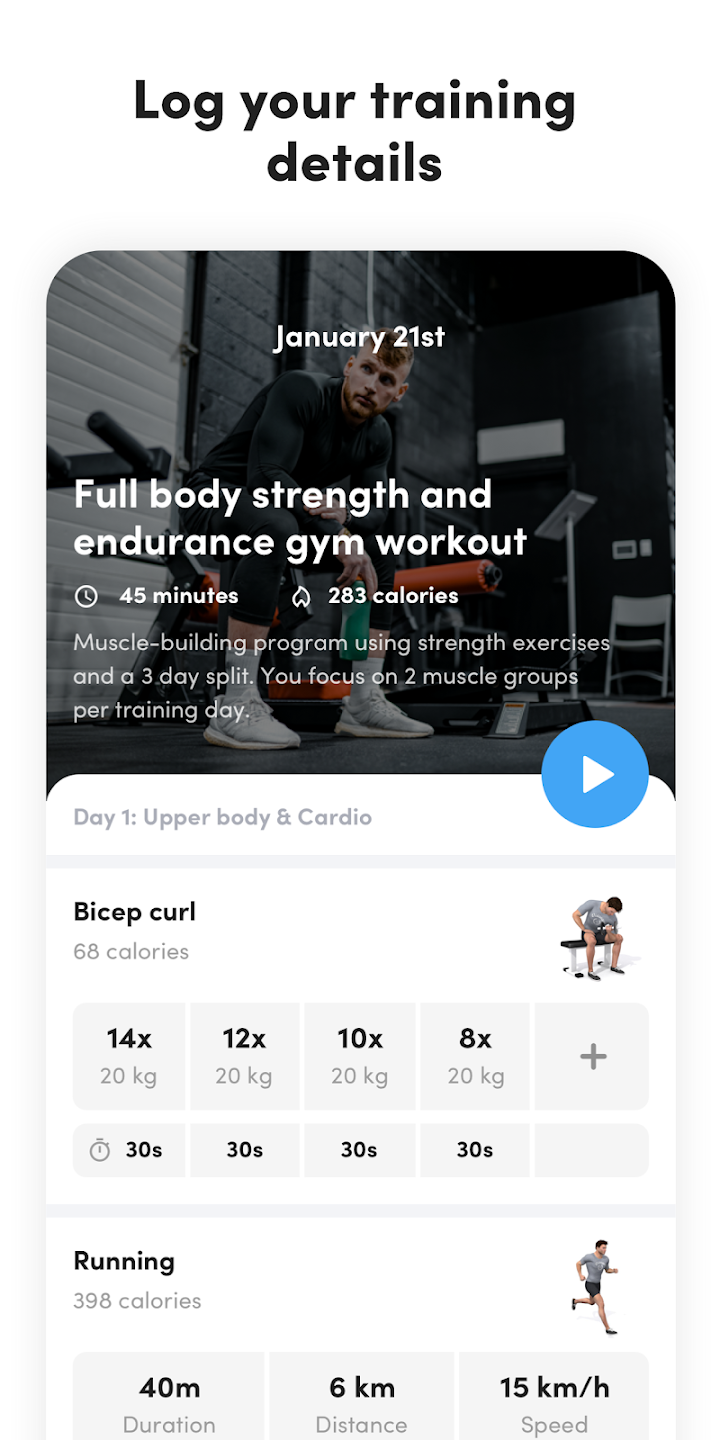
\includegraphics[width=\textwidth]{2-CompetitorsAnalysis/img/Virtualgym/Log.jpg}
        \caption{Log Interface}
        \label{fig:virtualgym_log}
    \end{subfigure}
    \caption{Virtualgym App Interface}
    \label{fig:virtualgym_app}
\end{figure}

\begin{table}[H]
    \centering
    \resizebox{\textwidth}{!}{
    \begin{tabular}{l c c c c}
        \toprule
        \textbf{Dimension} & \textbf{Virgin Active} & \textbf{EvolutionFit} & \textbf{Technogym} & \textbf{Virtuagym} \\
        \midrule
        Business Model / Price       & Included in Membership & Free for Users (B2B) & Freemium / Subs & Freemium / Subs \\
        Registration                 & Mandatory & Mandatory & Mandatory & Mandatory \\
        Target Audience              & Virgin Active Members & Affiliated Gym Members & B2B / B2C (All) & B2B / B2C (All) \\
        Supported Platforms          & iOS, Android & iOS, Android, Web & iOS, Android, Watch & iOS, Android, Web \\
        Downloads (Play Store)       & 5Mln+ & Not comparable (gym-distributed) & 1Mln+ & 5Mln+ \\
        Rating (Play Store)          & 4.6 & 3.4 & 4.8 & 4.7 \\
        Rating (App Store)           & 4.7 & 2.5 & 4.7 & 4.7 \\
        \bottomrule
    \end{tabular}
    }
    \vspace{0.2cm}
    \caption{Dimensions comparison of direct competitors}
    \label{tab:dimensions_competitors}
\end{table}

\vspace{0.5cm}

\begin{table}[H]
    \centering
    \resizebox{\textwidth}{!}{
    \begin{tabular}{l c c c c}
        \toprule
        \textbf{Feature} & \textbf{Virgin Active} & \textbf{EvolutionFit} & \textbf{Technogym} & \textbf{Virtuagym} \\
        \midrule
        Workout tracking \& statistics       & Yes & Yes & Yes & Yes \\
        Diet \& nutrition management         & No  & Yes & No  & Yes \\
        Class \& appointment booking         & Yes & Yes & Yes & Yes \\
        Digital facility access (QR/RFID)    & Yes & Yes & Yes & Yes \\
        Direct chat with professionals       & No  & Yes & No  & Yes \\
        Dedicated Admin/Staff dashboard      & No  & Yes & Yes & Yes \\
        \bottomrule
    \end{tabular}
    }
    \vspace{0.2cm}
    \caption{Features comparison of direct competitors}
    \label{tab:features_competitors}
\end{table}



\subsection{Indirect Competitors}\label{subsect:IndirectCompetitors}
As defined in our theoretical framework, indirect competitors are applications that target a similar user group but offer a different value proposition, or satisfy only a partial need. For TrainHub, these are applications and tools that focus exclusively on a single aspect of the user's fitness journey (e.g., only diet or only workout tracking) and lack any integration with the services of a physical gym facility.

Our research highlighted a strong fragmentation in the digital habits of gym-goers. We categorized these indirect competitors into four main groups:

\begin{itemize}
    \item \textbf{Workout Tracking (Hevy, GymLife, Bodymatica):}
    these applications allow users to build custom workout routines and track their weightlifting progress.
    \textit{Why they are indirect:} they operate as excellent standalone diaries, but they do not offer a direct, integrated communication channel with the user's actual Personal Trainer, nor do they support facility-specific features like class bookings or gym access;

    \item \textbf{Nutrition Tracking (MyFitnessPal, Yazio):}
    these are market leaders in their specific niche, highly specialized in calorie counting and macronutrient tracking.
    \textit{Why they are indirect:} they focus exclusively on the dietary aspect of fitness, completely detached from the user's workout routines and the gym's ecosystem;

    \item \textbf{Cardio \& General Tracking (Garmin Connect, Strava, Polar Flow, Suunto):}
    these platforms are deeply tied to wearable devices (smartwatches) and excel at tracking outdoor activities, heart rate, and overall health metrics.
    \textit{Why they are indirect:} they are generic health trackers. While extremely useful, they are entirely disconnected from the specific concepts of "gym management", "PT appointments", or "facility interaction";

    \item \textbf{Generic \& Analog Tools (Apple Notes, Excel/Numbers, PDFs, WhatsApp/Telegram, Emails):}
    interestingly, our market research revealed that a significant portion of both clients and professionals still rely heavily on these non-specific tools to log progress, share workout PDFs, and communicate. 
    \textit{Why they are indirect:} they represent the current, inefficient "status quo." Using three or four different generic apps to manage one fitness journey creates friction.
\end{itemize}

\paragraph{Key Takeaway}
The analysis of these indirect competitors strongly validates the core idea behind TrainHub. While users have access to excellent specialized tools, the real frustration lies in the fragmentation. TrainHub aims to beat this "status quo" by gathering the best aspects of these scattered tools and unifying them into a single, automated platform directly connected to the user's physical gym.

\subsection{Competitive Positioning}\label{subsect:CompetitorsConclusion}
The competitor analysis provided critical insights into the current landscape of fitness and gym management applications. As observed, the market is highly polarized: on one hand, there are robust, all-in-one direct competitors that either operate as closed ecosystems (e.g., Virgin Active) or as complex, heavy B2B solutions (e.g., Virtuagym). On the other hand, a vast array of indirect competitors offers excellent but fragmented tools, forcing users and professionals to rely on multiple apps, spreadsheets, and generic messaging platforms to manage a single fitness journey.

This fragmentation represents the exact market gap TrainHub aims to fill. By evaluating the strengths and weaknesses of both categories, we established a clear value proposition for our project. TrainHub will not overcomplicate the experience with excessive B2B management features, nor will it be just another standalone workout diary. Instead, it will be positioned as an intuitive, lightweight Progressive Web App (PWA) designed to seamlessly connect gym-goers with their facility and trusted professionals.

By successfully integrating workout tracking, professional dietary planning, facility access, and direct communication into one unified environment, TrainHub will solve the current "app fatigue" problem. Ultimately, this market validation confirms the actual need for our solution and provides a solid, data-driven foundation for the subsequent design and development phases.

\newpage
\section{User Research}\label{sect:UserResearch}

\subsection{Introduction}\label{subsect:UR_Introduction}
Following the market and competitor analysis, the next fundamental step in the design process of TrainHub was conducting comprehensive User Research. As established by the theoretical principles of mobile interaction design, engaging directly with potential users is crucial to fully understand their real needs, daily habits, and primary frustrations. 

To gather both quantitative and qualitative data, we designed and distributed a targeted questionnaire using Google Forms. Recognizing the dual-sided nature of our platform, the survey was carefully structured to accommodate differentiated paths for our two main user categories: gym members (clients) and fitness professionals (admins). 

The primary objective of this research phase was twofold: first, to empirically validate our initial assumptions regarding the preliminary features; second, to uncover the actual pain points caused by the current digital fragmentation in the fitness industry. The insights gathered from this questionnaire provided the necessary data-driven foundation to define realistic User Personas and formulate concrete User Scenarios, ultimately guiding the design and development of the application's interface.

\subsection{Questionnaire and Results}\label{subsect:QuestionnaireResults}
To empirically validate our design hypothesis, the Google Forms survey was distributed to a varied sample of individuals involved in the fitness ecosystem. The questionnaire collected a total of 76 valid responses. By utilizing conditional logic branches within the form, we ensured that both gym members and professionals could provide specific, highly relevant insights based on their distinct operational contexts.

\subsubsection{Demographics}\label{subsubsect:Demographics}

\begin{figure}[H]
    \centering
    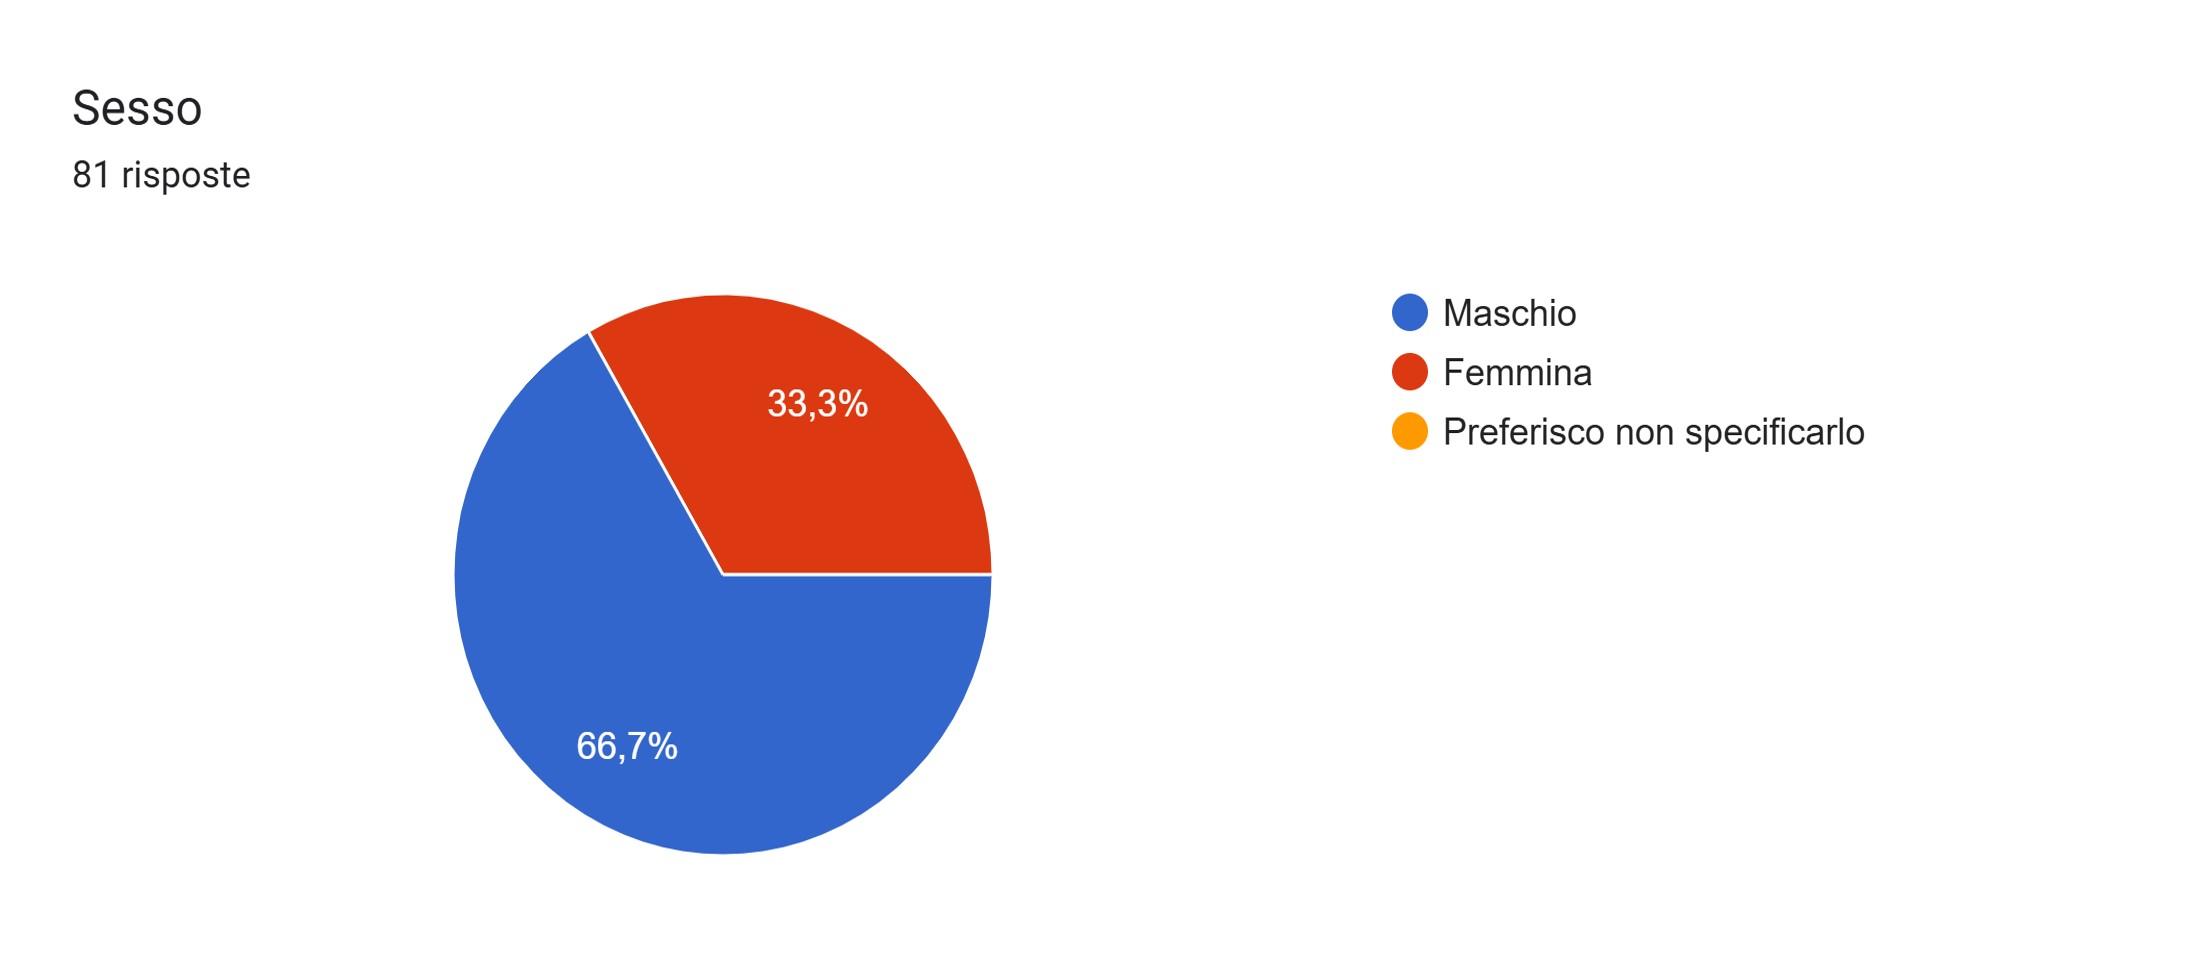
\includegraphics[width=0.8\textwidth]{3-UserResearch/img/Questionnaire/Demographics/Sesso.jpg}
    \caption{Gender distribution of the respondents.}
    \label{img:QuestionnaireGender}
\end{figure}

\begin{figure}[H]
    \centering
    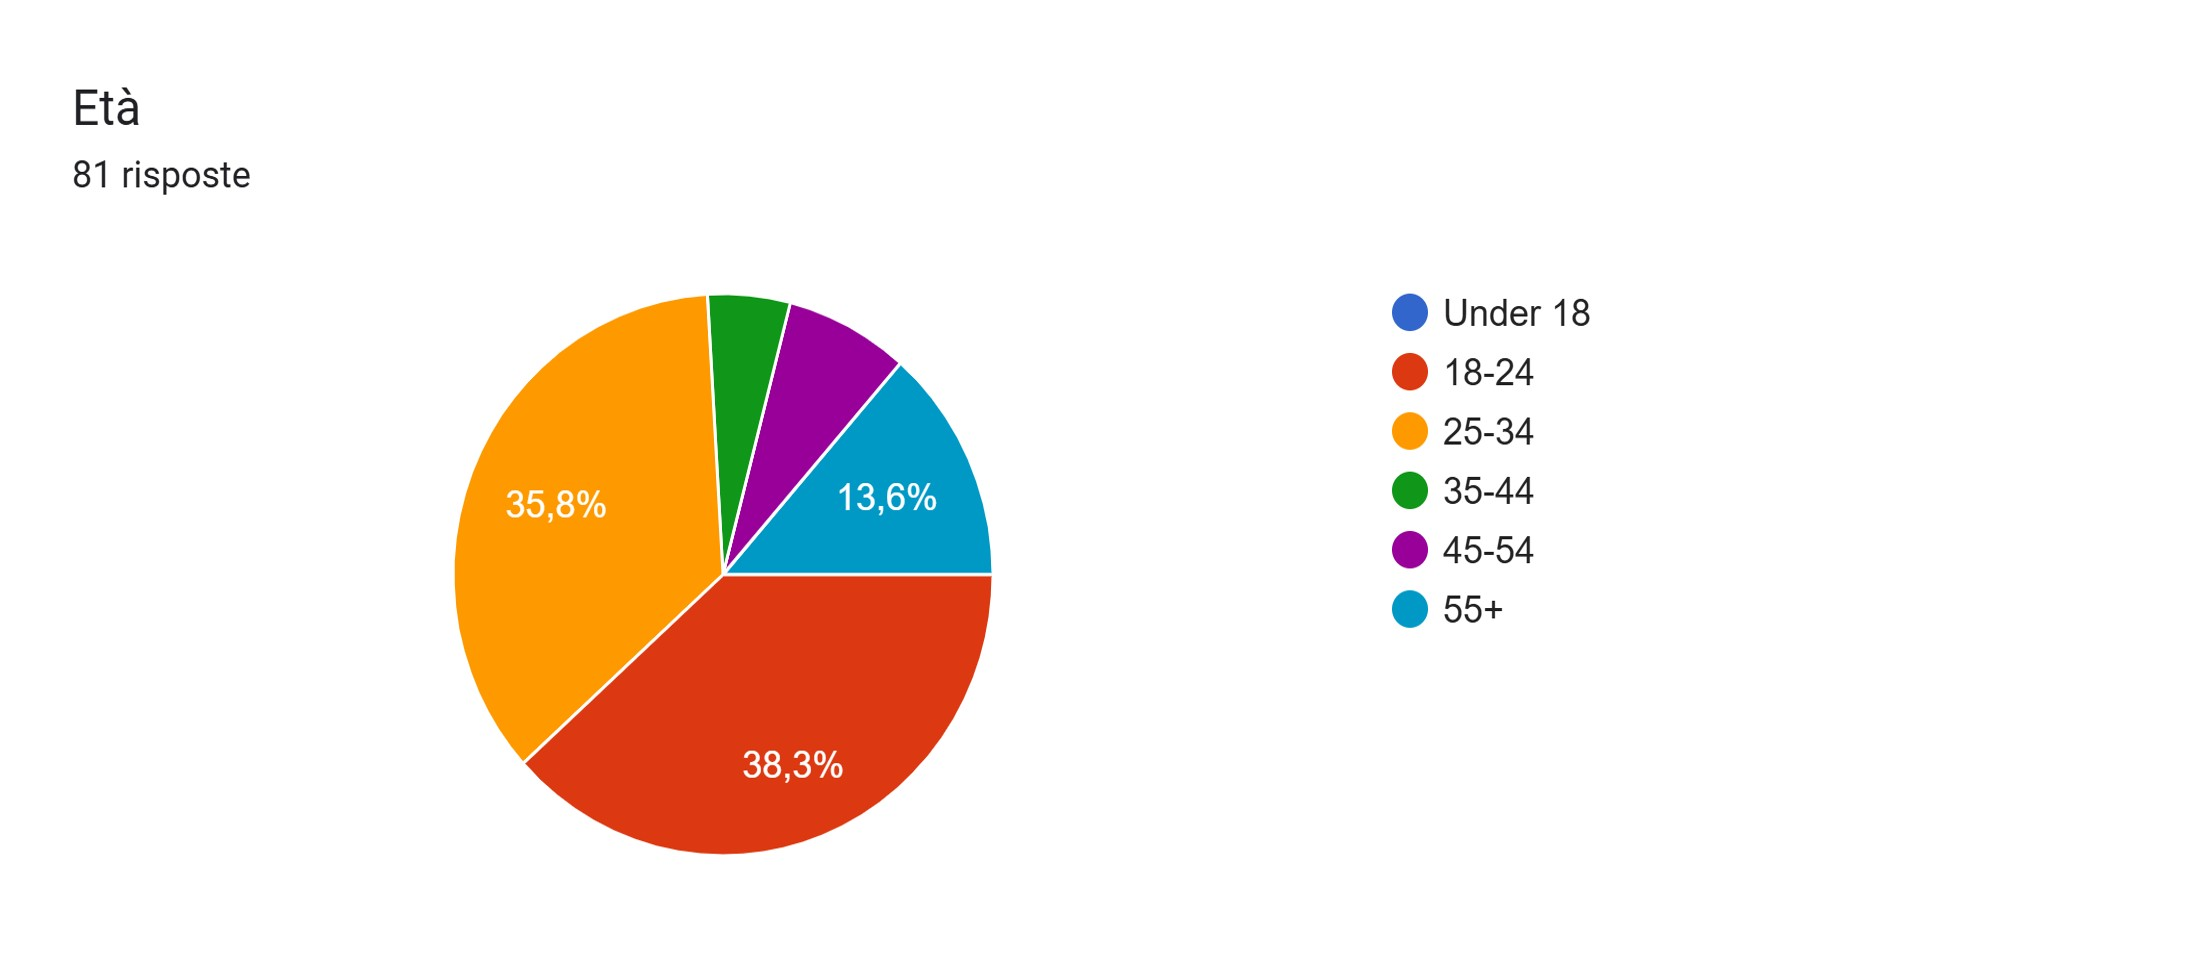
\includegraphics[width=0.8\textwidth]{3-UserResearch/img/Questionnaire/Demographics/Eta.jpg}
    \caption{Age distribution of the respondents.}
    \label{img:QuestionnaireAge}
\end{figure}

\begin{figure}[H]
    \centering
    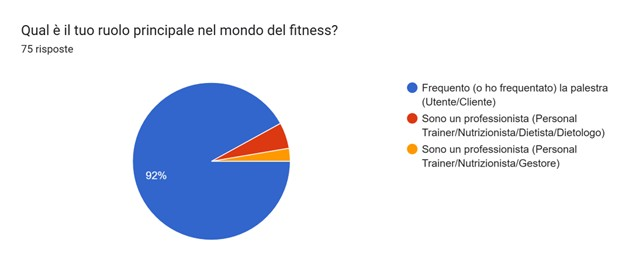
\includegraphics[width=0.8\textwidth]{3-UserResearch/img/Questionnaire/Demographics/Ruolo.jpg}
    \caption{Role distribution of the respondents.}
    \label{img:QuestionnaireRole}
\end{figure}

\textbf{Note: }The red and orange categories in the legend of Figure \ref{img:QuestionnaireRole} were split by Google Forms, but they actually represent the same group.

\vspace{0.3cm}
\textbf{Analysis of Demographics:} 
As shown in Figures \ref{img:QuestionnaireGender} and \ref{img:QuestionnaireAge}, the demographic profile of the respondents indicates a predominantly young adult audience, with the vast majority falling into the 18-24 and 25-34 age brackets. The sample of 76 respondents successfully captured insights from both sides of the market: exactly 92\% (70 individuals) identified as gym members (clients), while the remaining 8\% (6 individuals) are certified professionals (Personal Trainers, Nutritionists, and Dietitians). This specific distribution strongly mirrors the realistic proportions of a physical gym ecosystem, where a smaller, dedicated group of staff members manages a high volume of clients, ensuring that our feedback accurately reflects real-world market dynamics.


\subsubsection{Gym Members' Feedback}\label{subsubsect:GymMembers'Feedback}

\begin{figure}[H]
    \centering
    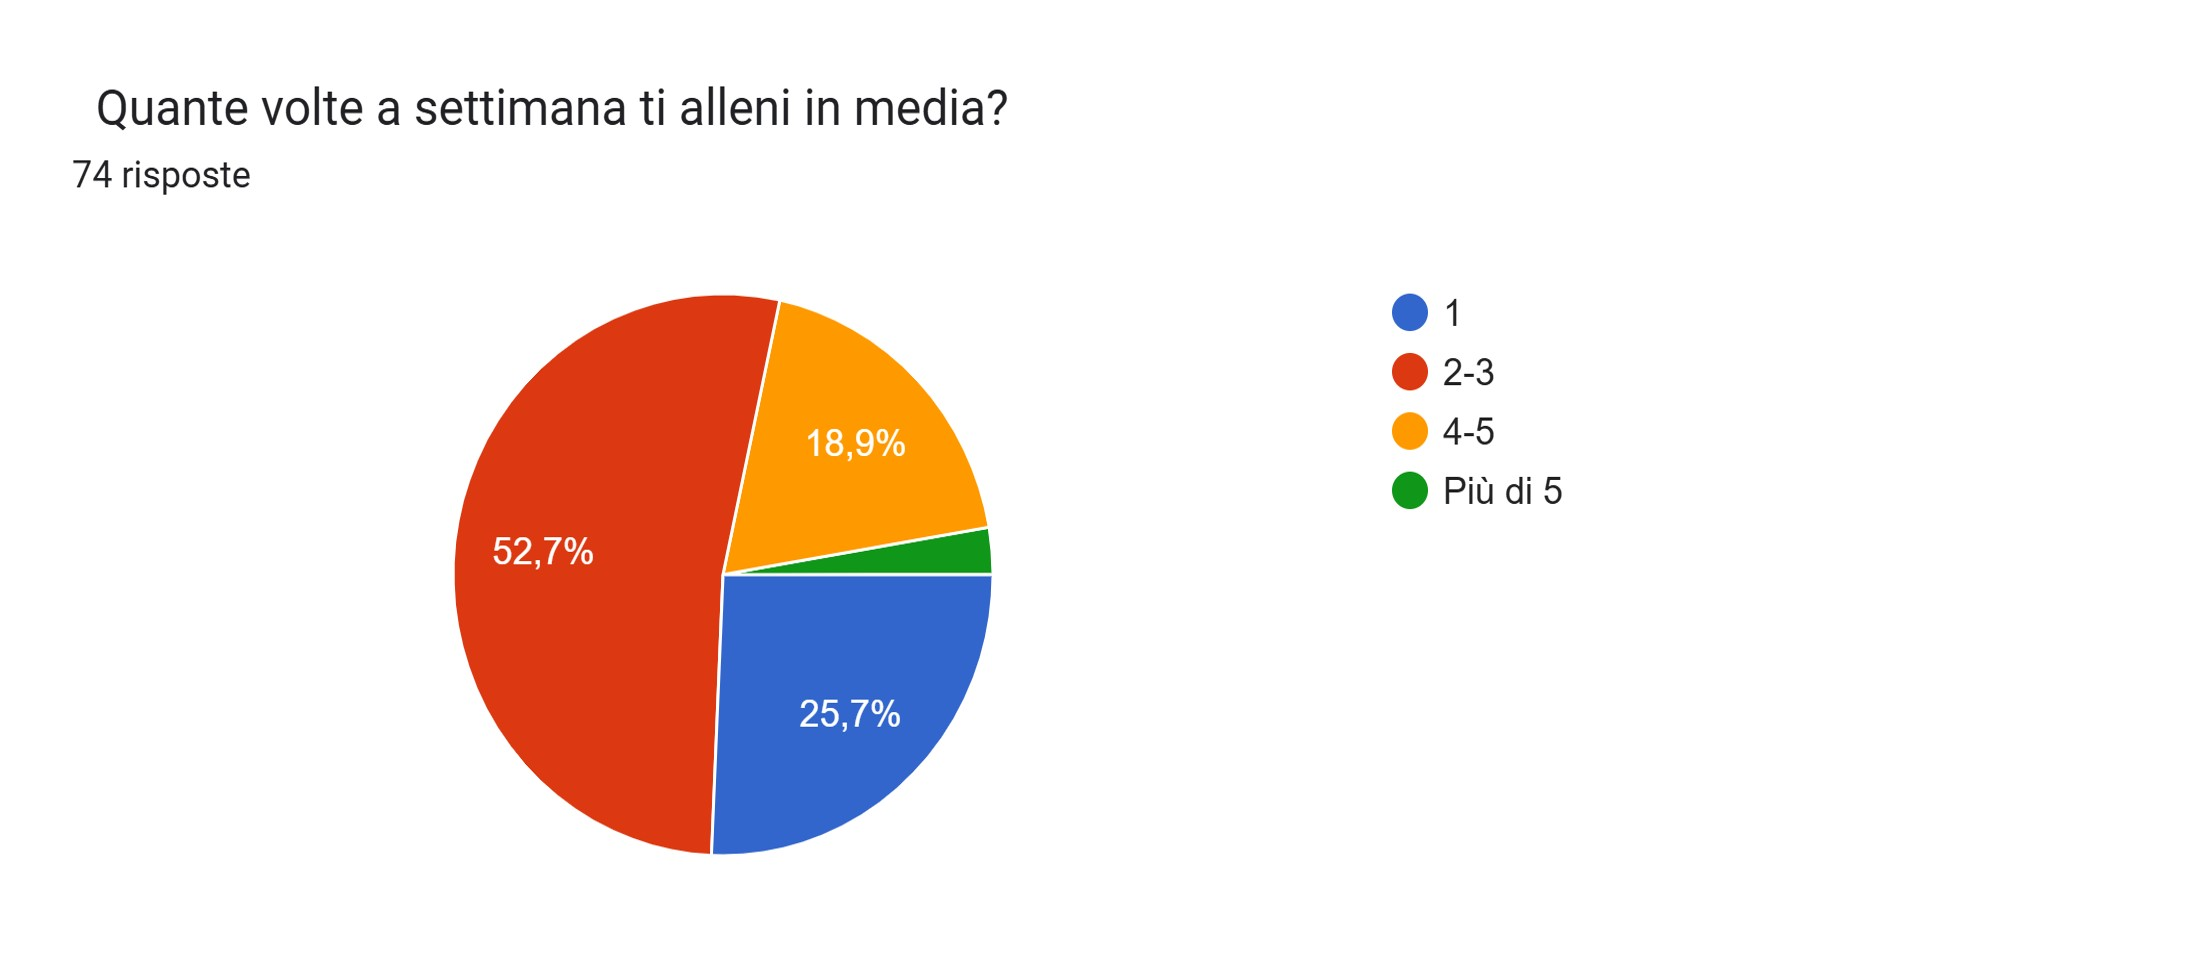
\includegraphics[width=0.8\textwidth]{3-UserResearch/img/Questionnaire/GymMembers/FrequenzaAllenamento.jpg}
    \caption{Frequency of training sessions.}
    \label{img:QuestionnaireFrequency}
\end{figure}

\begin{figure}[H]
    \centering
    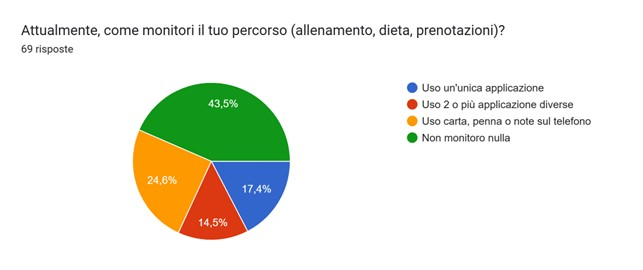
\includegraphics[width=0.8\textwidth]{3-UserResearch/img/Questionnaire/GymMembers/MonitoraggioAllenamento.jpg}
    \caption{Methods used by gym members to track their training sessions.}
    \label{img:QuestionnaireTracking}
\end{figure}

\begin{figure}[H]
    \centering
    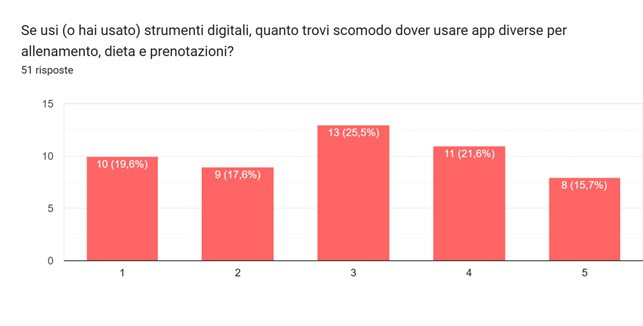
\includegraphics[width=0.8\textwidth]{3-UserResearch/img/Questionnaire/GymMembers/ScomoditaDiverseApp.jpg}
    \caption{Discomforts experienced by gym members when using different fitness apps.}
    \label{img:QuestionnaireDiscomfort}
\end{figure}

\begin{figure}[H]
    \centering
    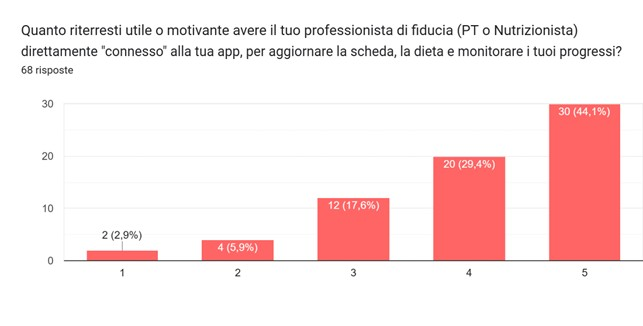
\includegraphics[width=0.8\textwidth]{3-UserResearch/img/Questionnaire/GymMembers/ConnnessioneProfessionista.jpg}
    \caption{Importance of connecting with a fitness professional.}
    \label{img:QuestionnaireConnection}
\end{figure}

\vspace{0.3cm}
\textbf{Analysis of Gym Members' Feedback:} 
The data reveals a highly active user base, with most participants training 2 to 5 times a week (Figure \ref{img:QuestionnaireFrequency}). Despite this dedication, Figure \ref{img:QuestionnaireTracking} highlights a critical inefficiency: a substantial portion of users still relies on analog methods (such as pen and paper or basic phone notes) or completely lacks a structured tracking system. Furthermore, many respondents suffer from the fragmentation of using multiple applications simultaneously. Consequently, Figure \ref{img:QuestionnaireDiscomfort} demonstrates the high frustration caused by this lack of integration. Most importantly, as depicted in Figure \ref{img:QuestionnaireConnection}, users expressed an overwhelming desire to have a direct, digital connection with their trusted professionals to receive updated diets and workout plans without constantly switching platforms.

\paragraph{Open Text Paragraph} Furthermore, the questionnaire included an open-ended question specifically directed at gym members, asking: \textit{"If you use one or more applications, please write their names in the field below"}. This specific inquiry proved to be extremely valuable for our overall market research. It allowed us to deepen and empirically validate the theoretical findings discussed during the Competitor Analysis phase (Chapter \ref{sect:CompetitorsAnalysis}). By collecting the exact names of the tools currently adopted by our real target audience, we were able to cross-reference our initial data, confirm our list of direct and indirect competitors, and ultimately prove the strong fragmentation that characterizes the current digital fitness landscape.


\subsubsection{Professionals' Feedback}\label{subsubsect:Professionals'Feedback}

\begin{figure}[H]
    \centering
    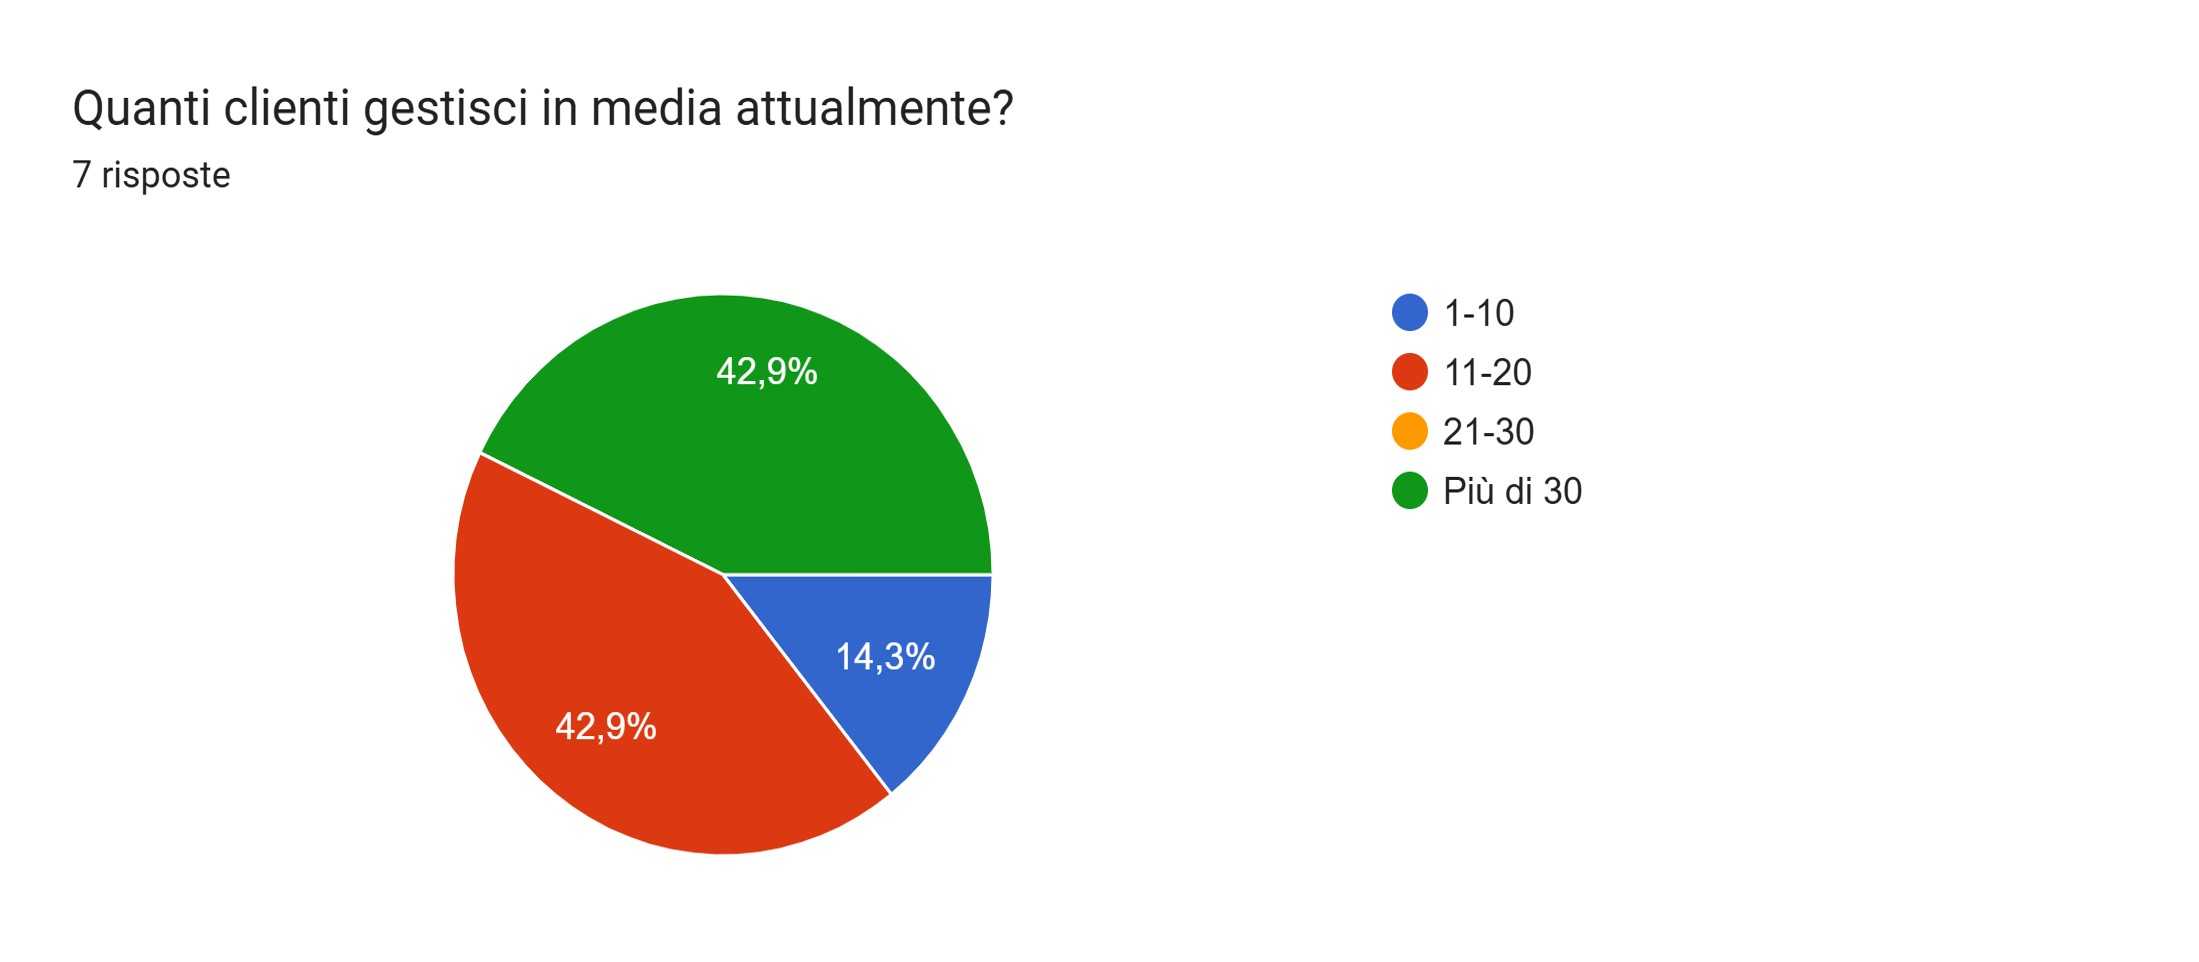
\includegraphics[width=0.8\textwidth]{3-UserResearch/img/Questionnaire/Professionists/NumeroClienti.jpg}
    \caption{Number of clients.}
    \label{img:QuestionnaireClients}
\end{figure}

\begin{figure}[H]
    \centering
    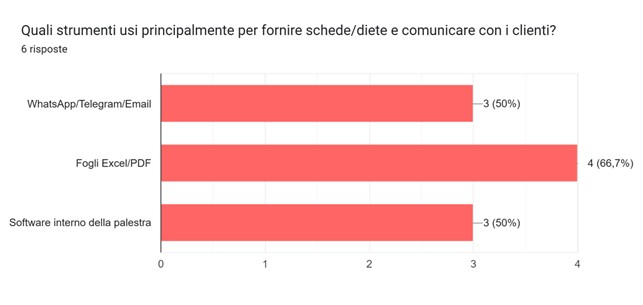
\includegraphics[width=0.8\textwidth]{3-UserResearch/img/Questionnaire/Professionists/StrumentiMonitoraggio.jpg}
    \caption{Tools used for monitoring clients.}
    \label{img:QuestionnaireMonitoring}
\end{figure}

\begin{figure}[H]
    \centering
    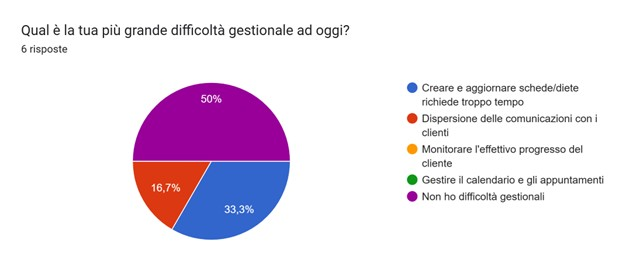
\includegraphics[width=0.8\textwidth]{3-UserResearch/img/Questionnaire/Professionists/DifficoltaGestionale.jpg}
    \caption{Challenges in client management.}
    \label{img:QuestionnaireChallenges}
\end{figure}

\vspace{0.3cm}
\textbf{Analysis of Professionals' Feedback:} 
The surveyed professionals manage varying client loads, ranging from a few individuals up to groups of over 50 clients (Figure \ref{img:QuestionnaireClients}). The core issue disrupting their workflow is clearly identified in Figure \ref{img:QuestionnaireMonitoring}: a heavy reliance on generic, non-specialized tools such as WhatsApp, Telegram, Emails, and Excel spreadsheets. Unsurprisingly, Figure \ref{img:QuestionnaireChallenges} confirms that their primary management challenges revolve around the dispersion of communications and the lack of constant, organized feedback from clients. Managing multiple user routines through chaotic messaging applications creates an unsustainable administrative burden, strongly proving the necessity for a centralized professional dashboard.


\subsubsection{User Expectations and Proposed Solutions}\label{subsubsect:CommonFeedback}

\begin{figure}[H]
    \centering
    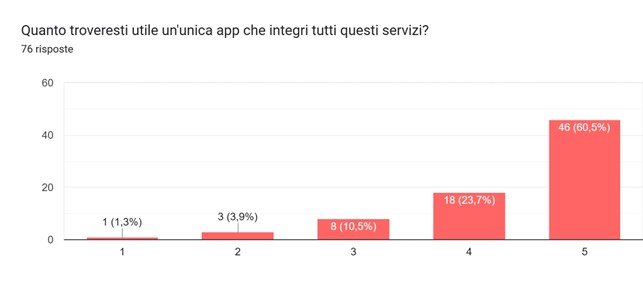
\includegraphics[width=0.8\textwidth]{3-UserResearch/img/Questionnaire/Common/UtilitaIntegrazione.jpg}
    \caption{Perceived usefulness of integrating a fitness app with a professional's monitoring system.}
    \label{img:QuestionnaireIntegration}
\end{figure}

\begin{figure}[H]
    \centering
    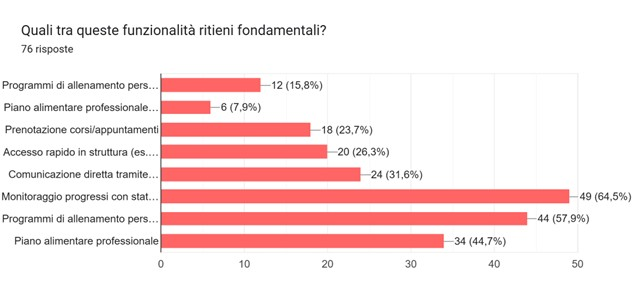
\includegraphics[width=0.8\textwidth]{3-UserResearch/img/Questionnaire/Common/FunzionalitaFondamentali.jpg}
    \caption{Essential features for a fitness app integrated with a professional's monitoring system.}
    \label{img:QuestionnaireEssentialFeatures}
\end{figure}

\vspace{0.3cm}
\textbf{Analysis of Expectations:} 
When asked about the potential utility of an all-in-one application that aggregates all these scattered services, the response was incredibly positive: Figure \ref{img:QuestionnaireIntegration} shows an overwhelming approval rating from both clients and professionals. Regarding the core functionalities (Figure \ref{img:QuestionnaireEssentialFeatures}), respondents pinpointed personalized workout tracking, professional diet management, and rapid digital facility access as absolute must-haves. These results definitively validate our initial feature assumptions and provide a clear, user-approved roadmap for TrainHub's core architecture.

\subsubsection{Qualitative Insights and Methodological Refinement}\label{subsubsect:QualitativeInsights}

\paragraph{Uncovering Unmet Needs and Feature Elicitation}
To maximize the value of our user research, the survey included an open-ended question designed to uncover specific pain points: \textit{"If you could improve or solve an impractical aspect related to the digital experience in the gym, what would it be?"}. Rather than directly asking participants what features they wanted, this problem-oriented approach allowed us to indirectly elicit new and unanticipated functional requirements. By focusing on the users' real frustrations and daily friction points, we gathered organic insights into unmet needs. This qualitative data significantly enriched the conceptualization of TrainHub, helping us identify and prioritize secondary features that could further elevate the platform's value proposition.

\paragraph{Methodological Feedback and Iterative Improvement}
Finally, acknowledging our ongoing learning process as university students, we added a concluding section dedicated entirely to methodological feedback: \textit{"Being a university project, we are still learning how to conduct user research. If you found any question unclear or hard to interpret, please let us know. Every feedback is gold to us!"}. This meta-research inquiry proved to be incredibly valuable in practice. The constructive criticism received from the earliest respondents highlighted minor ambiguities in our initial phrasing. Consequently, we adopted an agile and iterative approach, actively fine-tuning and adjusting the questionnaire during the data collection phase. This continuous refinement ensured maximum clarity for subsequent participants, thereby increasing the overall reliability and accuracy of our final dataset.
\subsection{Affinity Diagram}\label{subsect:AffinityDiagram}
Following the collection of raw data from the survey, we applied the Affinity Diagram methodology to systematically organize facts, opinions, and insights. This collaborative UX mapping activity was executed through a structured 8-step process to synthesize the research findings before defining the User Personas.

\paragraph{Steps 1 \& 2: Data Collection and Sticky Notes Generation}
We began by extracting the most relevant qualitative and quantitative information from the 81 valid questionnaire responses. We translated these data points into virtual sticky notes using \textbf{Figma}. The notes included direct quotes, statistics, and recurring pain points. For instance, client-side notes highlighted phrases like \textit{"I use paper, pen, or phone notes to track my workouts"} or \textit{"Switching between multiple apps for workouts and diets is highly frustrating,"} while professional-side notes emphasized \textit{"WhatsApp and Excel are chaotic for managing multiple clients."}

\paragraph{Steps 3, 4 \& 5: Clustering, Labeling, and Combining}
Once the digital board was populated, we grouped the notes into clusters based on natural relationships and labeled them according to their core themes. By combining similar concepts, three overarching macro-themes emerged:
\begin{itemize}
    \item \textbf{The Burden of Digital Fragmentation:} a massive cluster formed around the inefficiency of current tracking methods. Sticky notes indicating the use of pen and paper, phone notes, and the simultaneous use of multiple apps were combined under this theme. The high frustration scores recorded in the survey strongly validated this label;
    \item \textbf{Inefficient B2C Communication:} this cluster grouped the professionals' administrative struggles (e.g., relying on generic messaging apps) with the clients' desire for a stronger, digital connection with their Personal Trainers. It highlighted the friction in exchanging feedback and updating diet/workout plans;
    \item \textbf{The "All-in-One" Demand:} a solution-oriented cluster aggregating the highly requested core features: unified workout tracking, integrated diet management, and digital facility access via QR code. 
\end{itemize}

\begin{figure}[H]
    \centering
    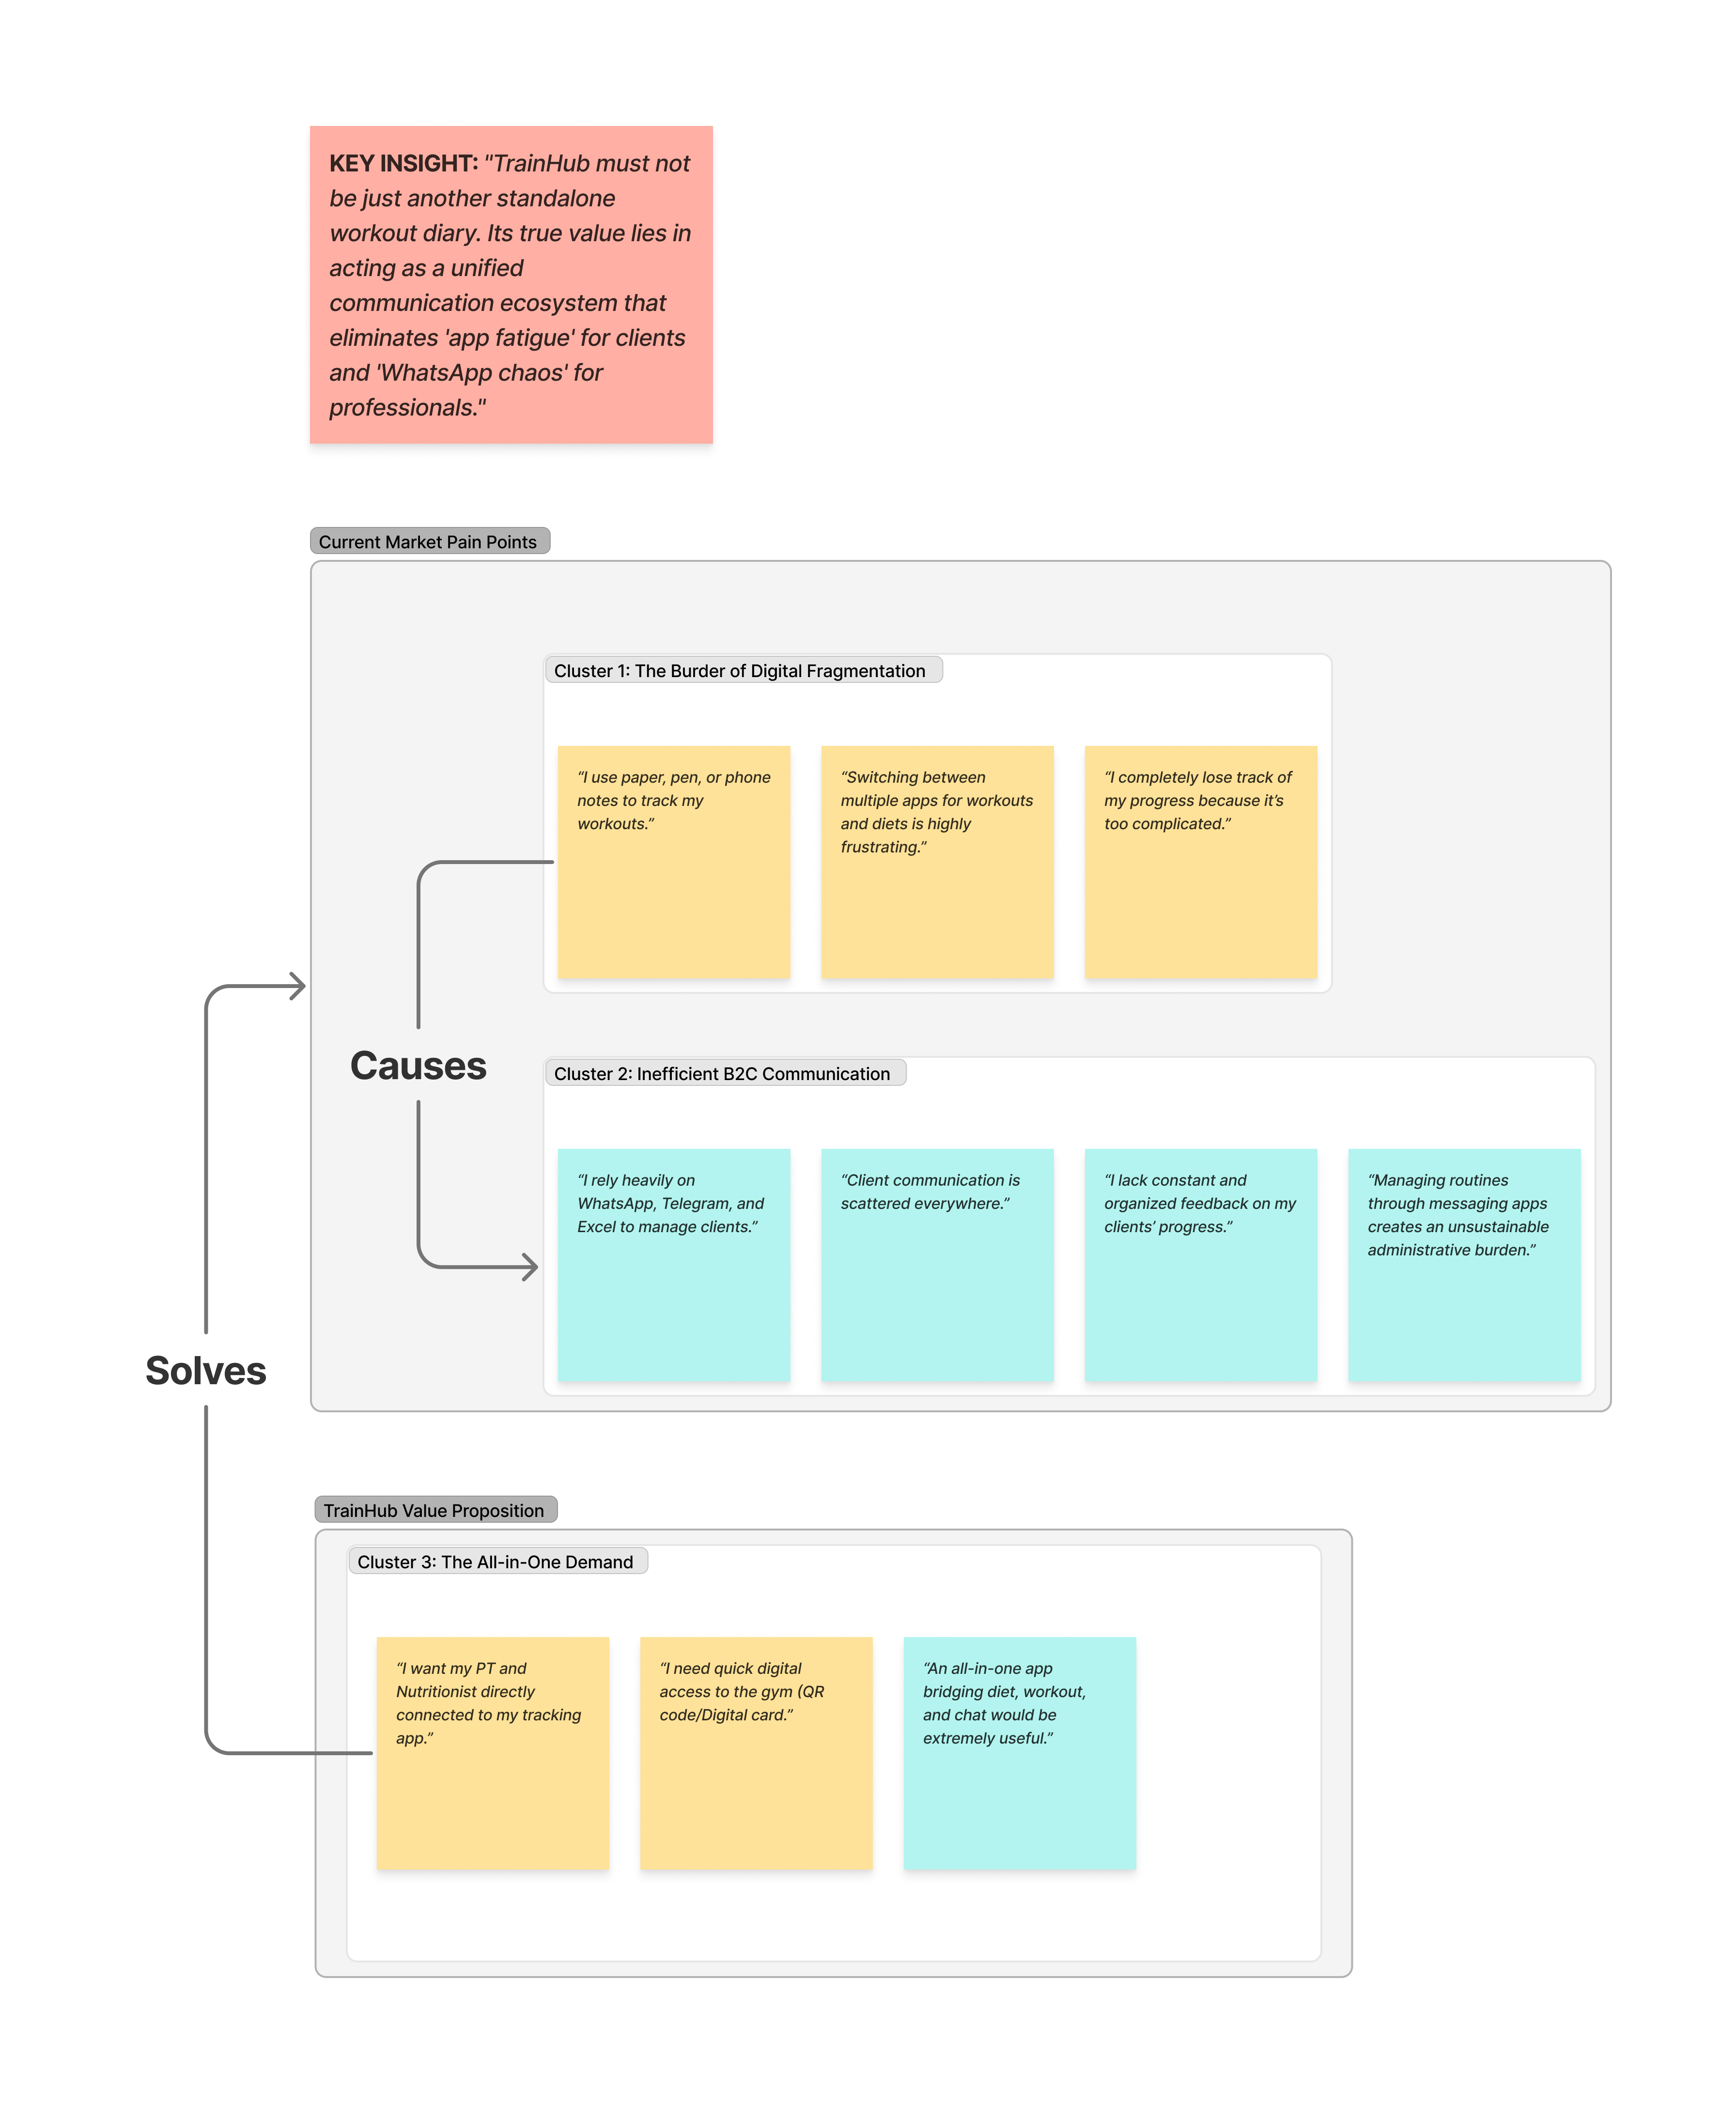
\includegraphics[width=0.9\textwidth]{3-UserResearch/img/AffinityDiagram/AffinityDiagram.jpg}
    \caption{Affinity Diagram board developed in Figma containing the clustered sticky notes.}
    \label{img:AffinityDiagramBoard}
\end{figure}

\paragraph{Step 6: Linking Dependencies}
After defining the macro-themes, we mapped the dependencies between the clusters. The structural link became evident: the \textit{Burden of Digital Fragmentation} (cause) directly forces professionals to resort to \textit{Inefficient B2C Communication} (effect), leading to poor tracking and frustrated users. The \textit{"All-in-One" Demand} acts as the structural bridge capable of resolving these dependencies by unifying the ecosystem.

\paragraph{Steps 7 \& 8: Interpretation and Documentation}
The final interpretation of this affinity mapping exercise provided a clear design directive. The diagram confirmed that TrainHub's core value does not simply lie in offering a digital workout diary, but rather in acting as a centralized communication hub that eliminates the "app fatigue". Documenting this process allowed us to confidently transition from raw, scattered survey data to well-defined, evidence-based user profiles. The insights finalized in this section directly shaped the goals and frustrations of the User Personas presented in the following paragraphs.

\subsection{User Personas}\label{subsect:Personas}

\begin{figure}[H]
    \centering
    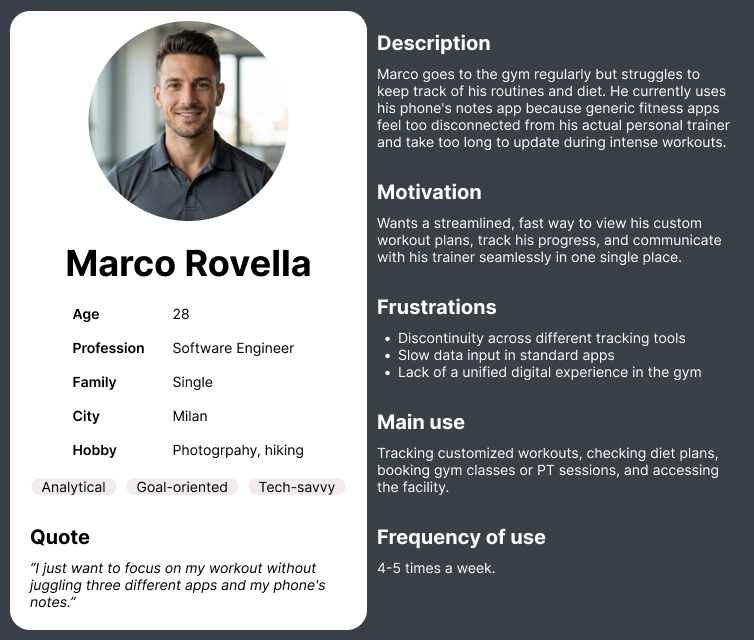
\includegraphics[width=0.8\textwidth]{3-UserResearch/img/Personas/Persona1.jpg}
     \caption{Persona 1: Young Gym Member.}
     \label{fig:Persona1}
\end{figure}

\begin{figure}[H]
    \centering
    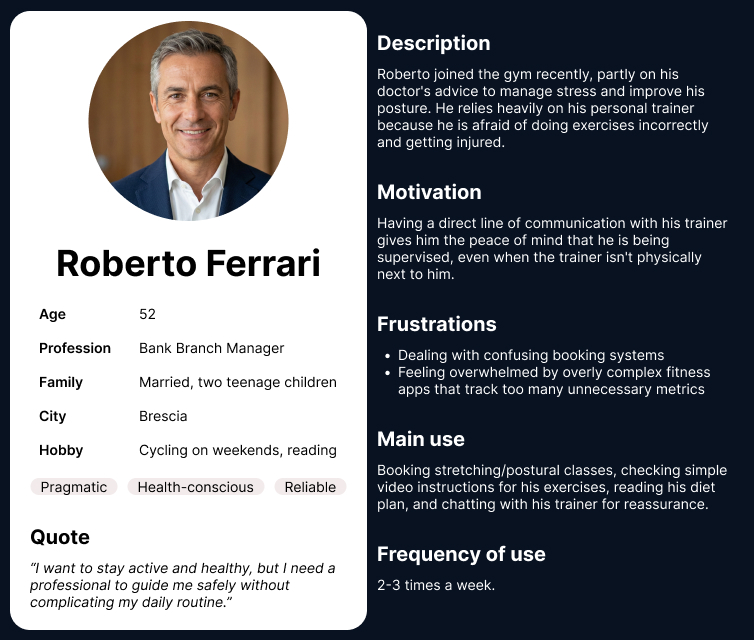
\includegraphics[width=0.8\textwidth]{3-UserResearch/img/Personas/Persona2.jpg}
     \caption{Persona 2: Senior Gym Member.}
     \label{fig:Persona2}
\end{figure}

\begin{figure}[H]
    \centering
    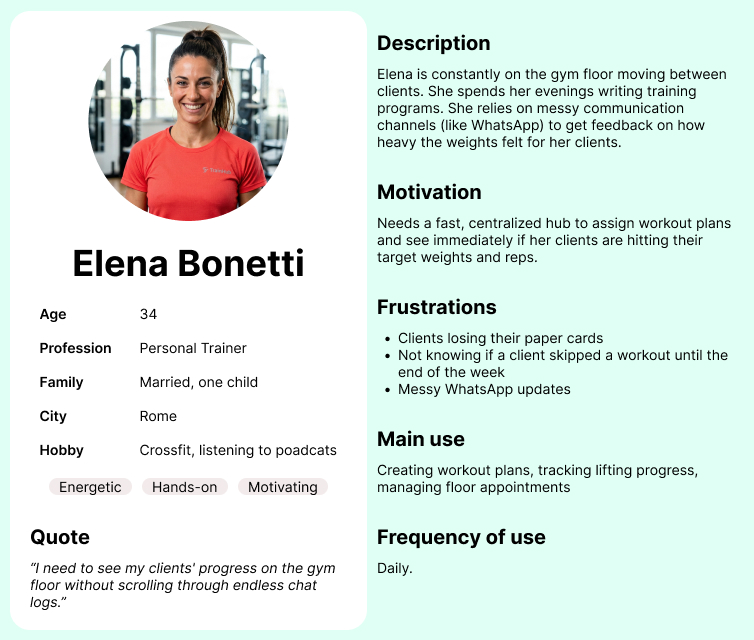
\includegraphics[width=0.8\textwidth]{3-UserResearch/img/Personas/Persona3.jpg}
     \caption{Persona 3: Personal Trainer.}
     \label{fig:Persona3}
\end{figure}

\begin{figure}[H]
    \centering
    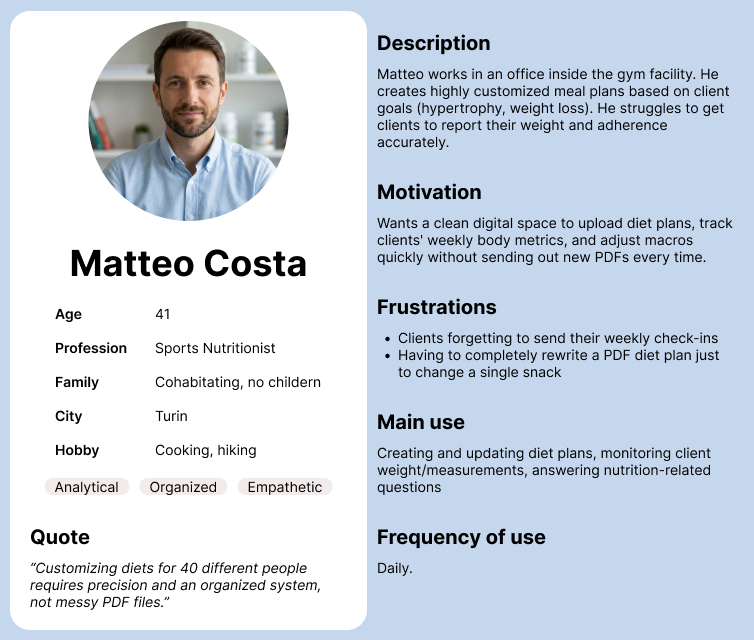
\includegraphics[width=0.8\textwidth]{3-UserResearch/img/Personas/Persona4.jpg}
     \caption{Persona 4: Nutritionist.}
     \label{fig:Persona4}
\end{figure}
\subsection{User Scenarios}\label{subsect:Scenarios}

\paragraph{Scenario 1: Marco Rovella (Young Gym Member)}Marco is in the weight room, in the middle of an intense workout, with limited time before heading back to the office. Marco needs to log the weights for his main exercise (Bench Press) as quickly as possible so he doesn't lose his focus.
Instead of opening his phone's notes app, he unlocks his screen and opens TrainHub, which immediately display today's routine. With a couple of quick taps on the “+” and “-” buttons, he confirms the pre-filled weights assigned by his PT based on his last session, marks the set as complete, and immediately moves on to the next exercise, receiving a small virtual badge for his consistency.

\paragraph{Scenario 2: Roberto Ferrari (Senior Gym Member)}It is Tuesday evening and Roberto is at home, relaxing on the couch after dinner. Roberto wants to prepare for tomorrow's workout and make sure he performs the exercises correctly to avoid hurting his back.
He opens the TrainHub app on his smartphone and he accesses his customized workout plan and watches a short video demonstration of an assigned exercise. Feeling a bit unsure about a specific movement, he uses the app's built-in chat to send a quick message to his PT (Elena), asking if the movement is appropriate for his level, and immediately feels reassured.

\paragraph{Scenario 3: Elena Bonetti (Personal Trainer)}Elena is on the gym floor, enjoying a short 5-minute break between one client and the next. Elena needs to monitor the progress of her clients who are working out independently to see if the assigned weights are appropriate. She pulls her phone out of her pocket and opens the TrainHub Admin dashboard. She sees a notification indicating that Marco has just completed his workout, hitting his target weights. Without having to open messy WhatsApp chats or Excel spreadsheets, Elena taps on Marco's profile and directly modifies the parameters of his routine for the following week, slightly increasing the load. She saves the changes is seconds, ready to welcome her next in-person client.

\paragraph{Scenario 4: Matteo Costa (Nutritionist)}It is Friday morning and Matteo is in his tidy offce inside the fitness facility. Matteo must analyze his clients' weekly weight check-ins and update their diet plans ahead of the weekend.
He logs into the TrainHub web app from his laptop. His main dashboard displays an automated summary showing who has logged their weight and who hasn't. Noticing that Roberto has entered his data but hit a plateau, Matteo accesses his digital nutrition plan and quickly adjusts the carbohydrate macros for his dinners. With a single click, he saves and publishes the new diet without needing to generate or email any PDF files. The system automatically sends a push notification to Roberto.
\newpage
\section{Application Design}\label{sect:ApplicationDesign}
% Paragrafo di apertura, sul modello di BookIT/Hammami_Hub: come si è passati
% dalla ricerca utenti (cap. 3) alla progettazione, strumenti usati (Figma),
% e rimando alle sottosezioni sotto.

\subsection{From Research to Design}\label{subsect:FromResearchToDesign}
% Breve: quali funzionalità il cap. 3 ha confermato/scartato, ponte diretto
% alle Personas/Scenarios/Affinity Diagram del cap. 3 (sul modello di BookIT
% 4.1 "Revisione delle funzionalità").

\subsection{Navigation Map}\label{subsect:NavigationMap}
% Intro breve: due alberi di navigazione, /m/ (membro) e /p/ (professionista) --
% vedi sezione 4 di docs/superpowers/specs/2026-07-27-trainhub-design.md.

\subsubsection{Paper Navigation Map}\label{subsubsect:PaperNavigationMap}
% Foto della mappa a post-it. doc/trainhub.md è la bozza iniziale (ora
% superseded) -- può valere come sostituto se le foto cartacee non esistono.

\subsubsection{Digital Navigation Map}\label{subsubsect:DigitalNavigationMap}
% Export Figma/diagramma della navigation map digitale.

\subsection{Paper Prototype}\label{subsect:PaperPrototype}

The paper prototype was used to verify content placement and the number of actions required to complete the scenarios from Chapter 3 before visual details were introduced. At this stage we also identified recurring elements such as the header, bottom navigation, cards, status labels, calendar cells, and primary actions. The sketches are grouped by task below, following the same division later used in the digital prototype.

\paragraph{Common Screens}

The first sketches defined the shared authentication entry point and the two Home screens (Figure \ref{fig:paperCommonScreens}). Login and password recovery use the same structure for both roles, while the Home alternatives introduce the different priorities immediately after access: the member sees personal activities, whereas the professional sees the daily client agenda.

\begin{figure}[H]
    \centering
    \begin{subfigure}[c]{0.52\textwidth}
        \centering
        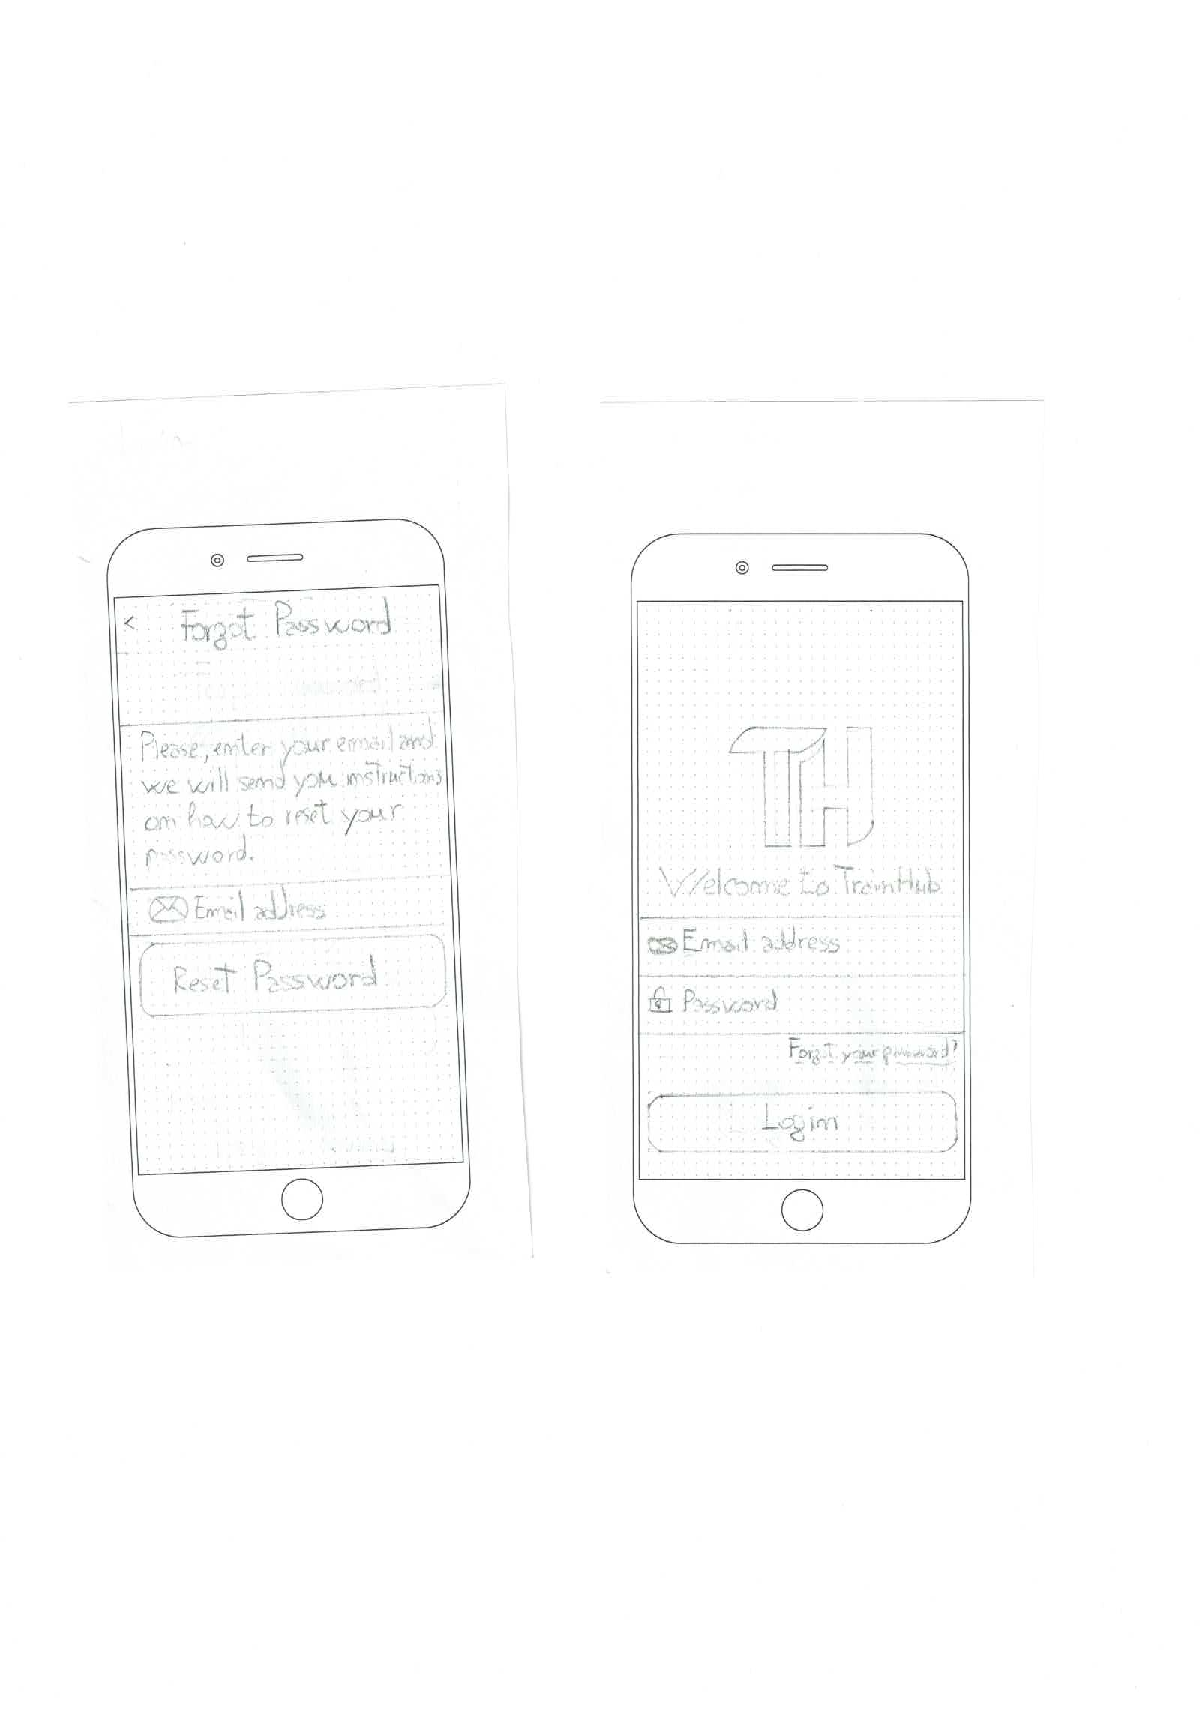
\includegraphics[width=\linewidth,trim=24bp 145bp 60bp 165bp,clip]{4-ApplicationDesign/img/PaperPrototype/paper-authentication.pdf}
        \caption{Authentication.}
    \end{subfigure}

    \vspace{0.35cm}
    \begin{subfigure}[c]{0.52\textwidth}
        \centering
        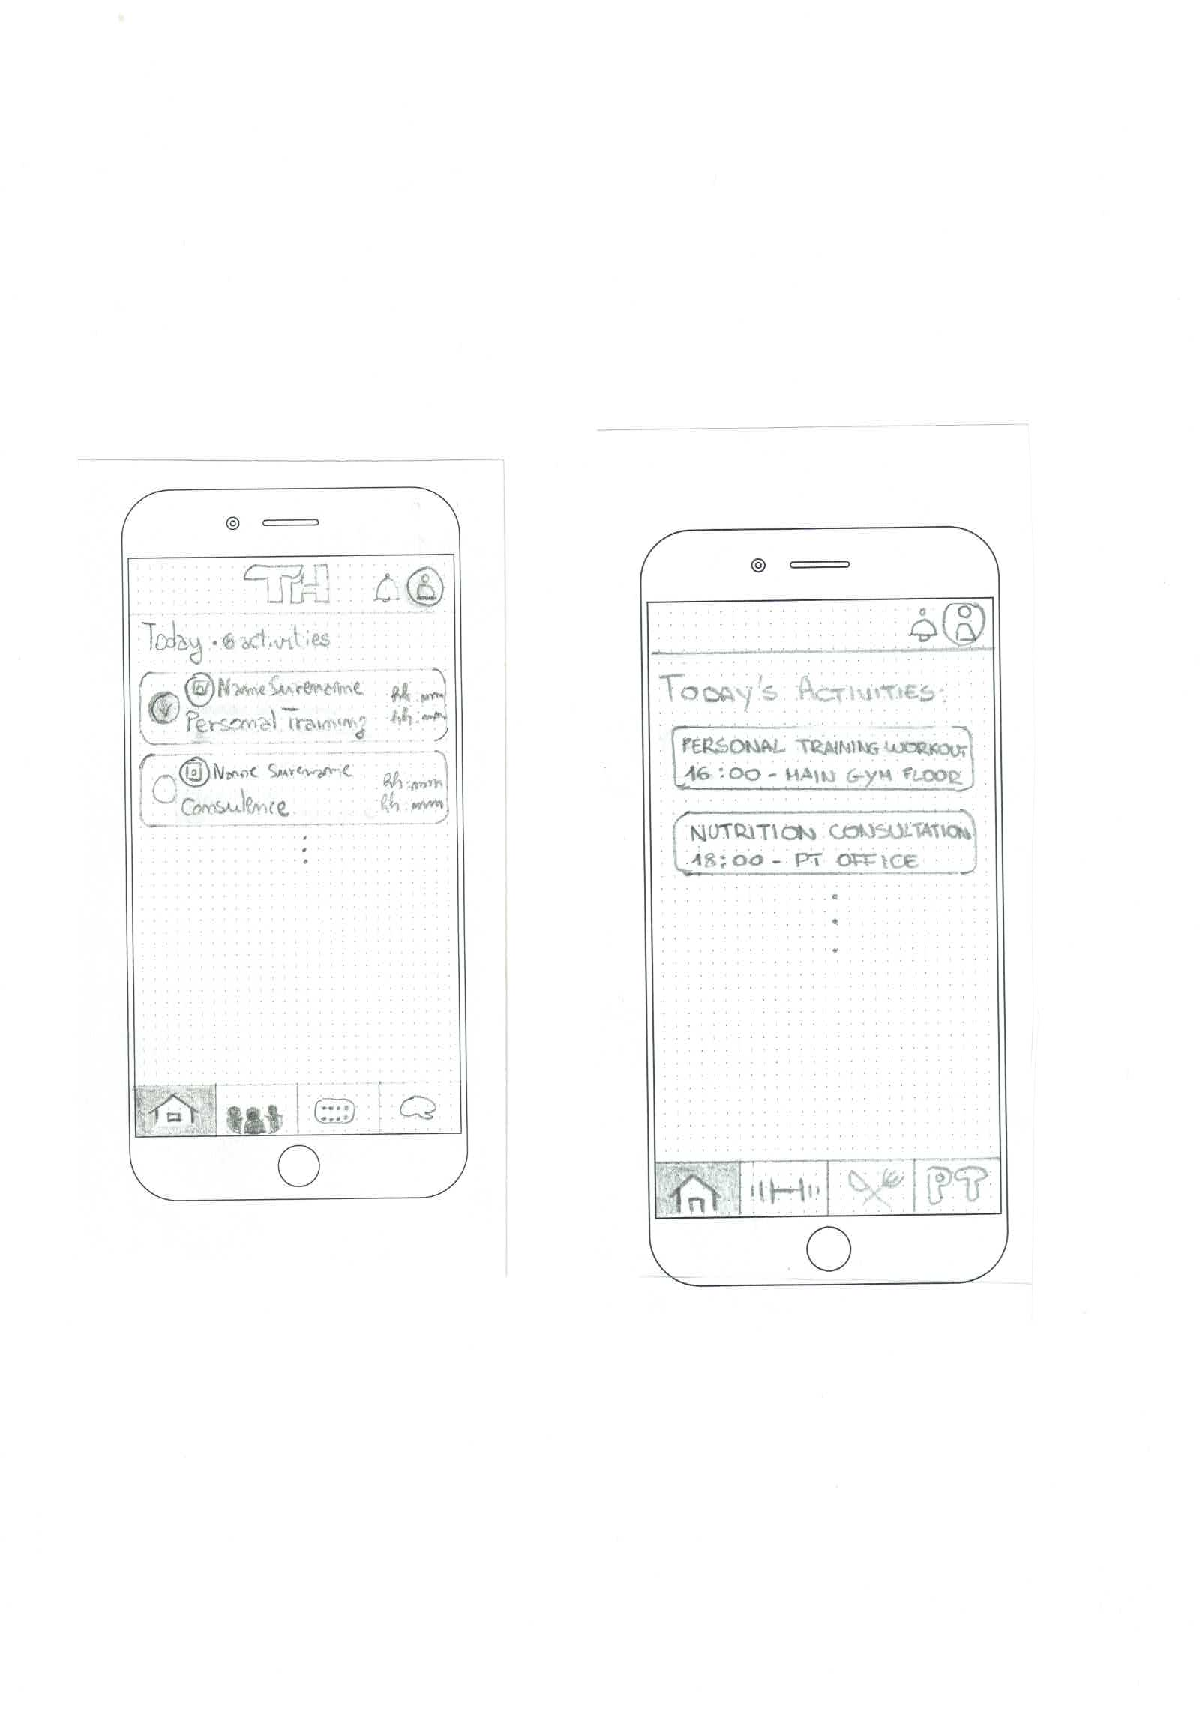
\includegraphics[width=\linewidth,trim=24bp 155bp 36bp 195bp,clip]{4-ApplicationDesign/img/PaperPrototype/paper-role-homes.pdf}
        \caption{Role-specific Home screens.}
    \end{subfigure}
    \caption{Shared entry screens in the paper prototype.}
    \label{fig:paperCommonScreens}
\end{figure}

\clearpage
\paragraph{Member Screens}

The member sketches were grouped around the four principal destinations. Workout moves from the plan list to session details and set recording (Figure \ref{fig:paperMemberWorkout}); Nutrition uses a shorter path from the assigned plan to its meals (Figure \ref{fig:paperMemberNutrition}). Personal Trainer combines professional selection, appointments, booking, and chat (Figures \ref{fig:paperMemberTrainer} and \ref{fig:paperMemberBooking}), while Profile collects access, subscription, and reward information (Figure \ref{fig:paperMemberProfile}).

\begin{figure}[H]
    \centering
    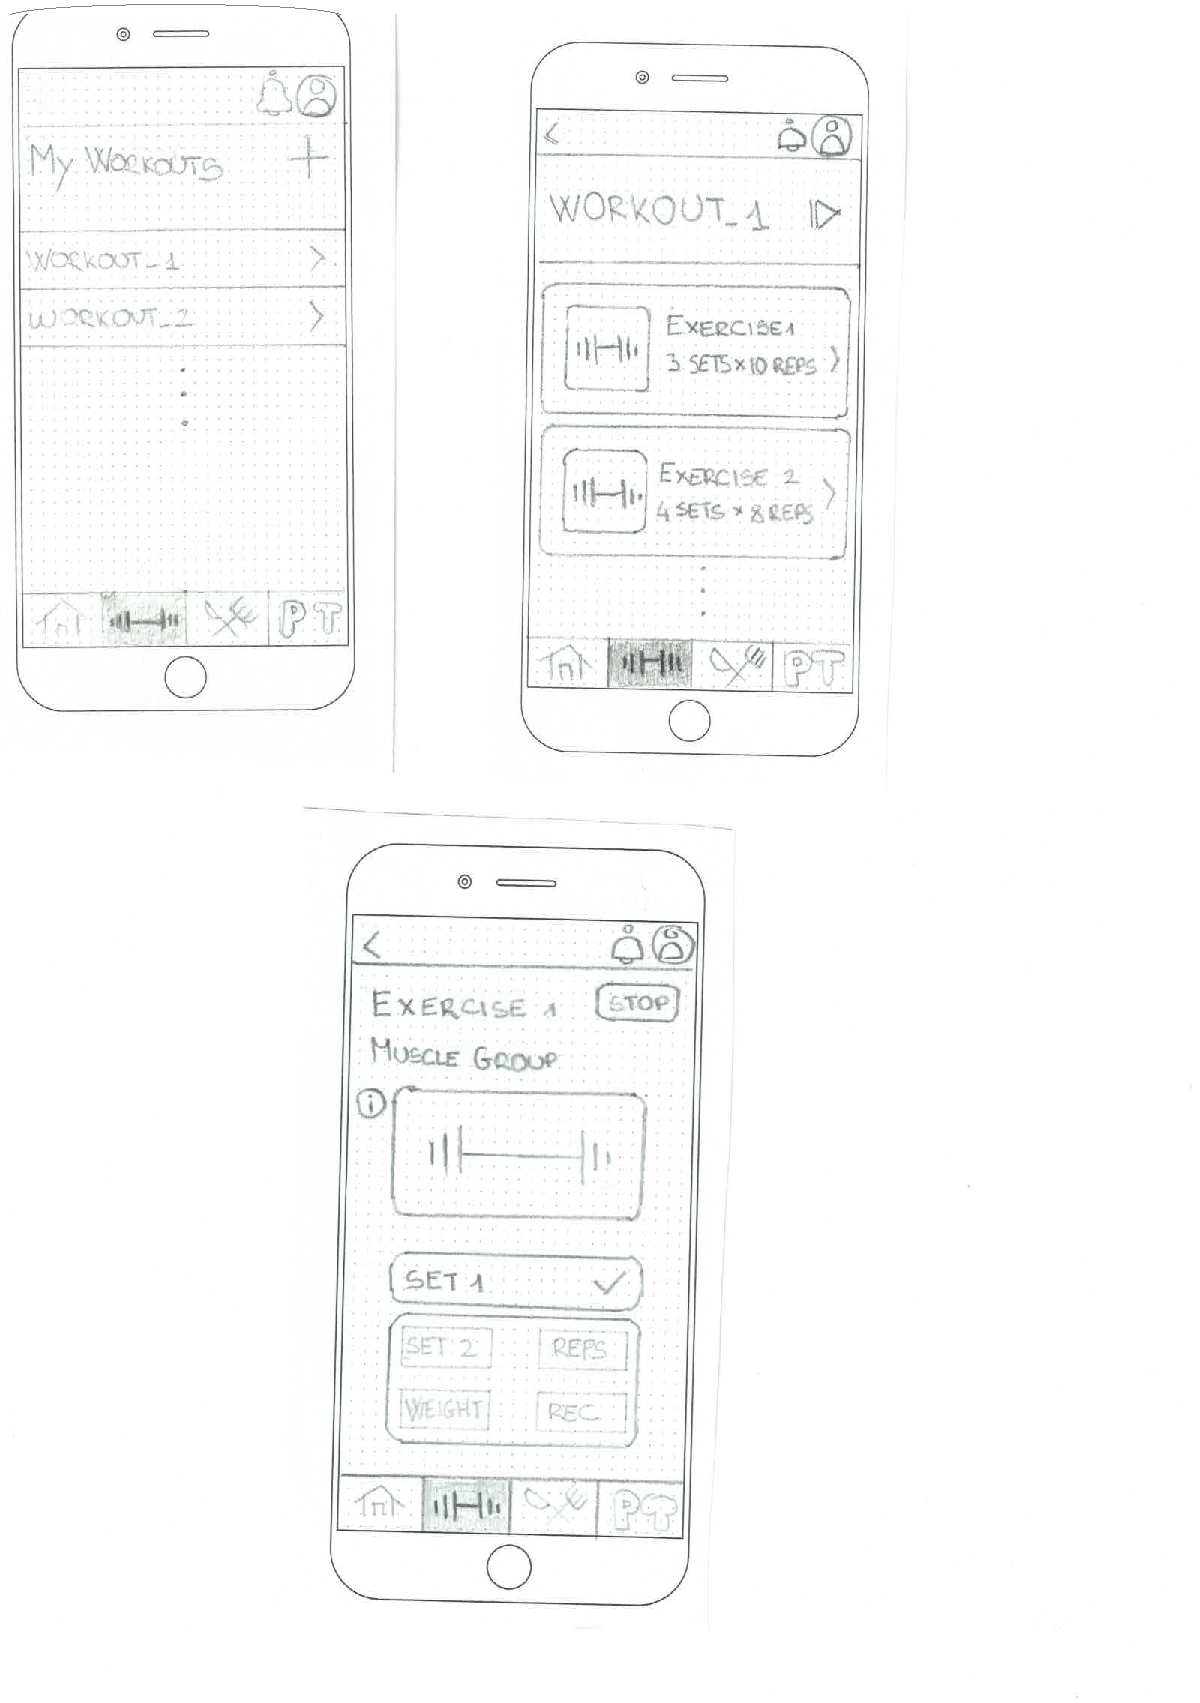
\includegraphics[width=0.62\textwidth]{4-ApplicationDesign/img/PaperPrototype/paper-member-workout-clean.pdf}
    \caption{Workout exploration and set recording.}
    \label{fig:paperMemberWorkout}
\end{figure}

\clearpage
\begin{figure}[H]
    \centering
    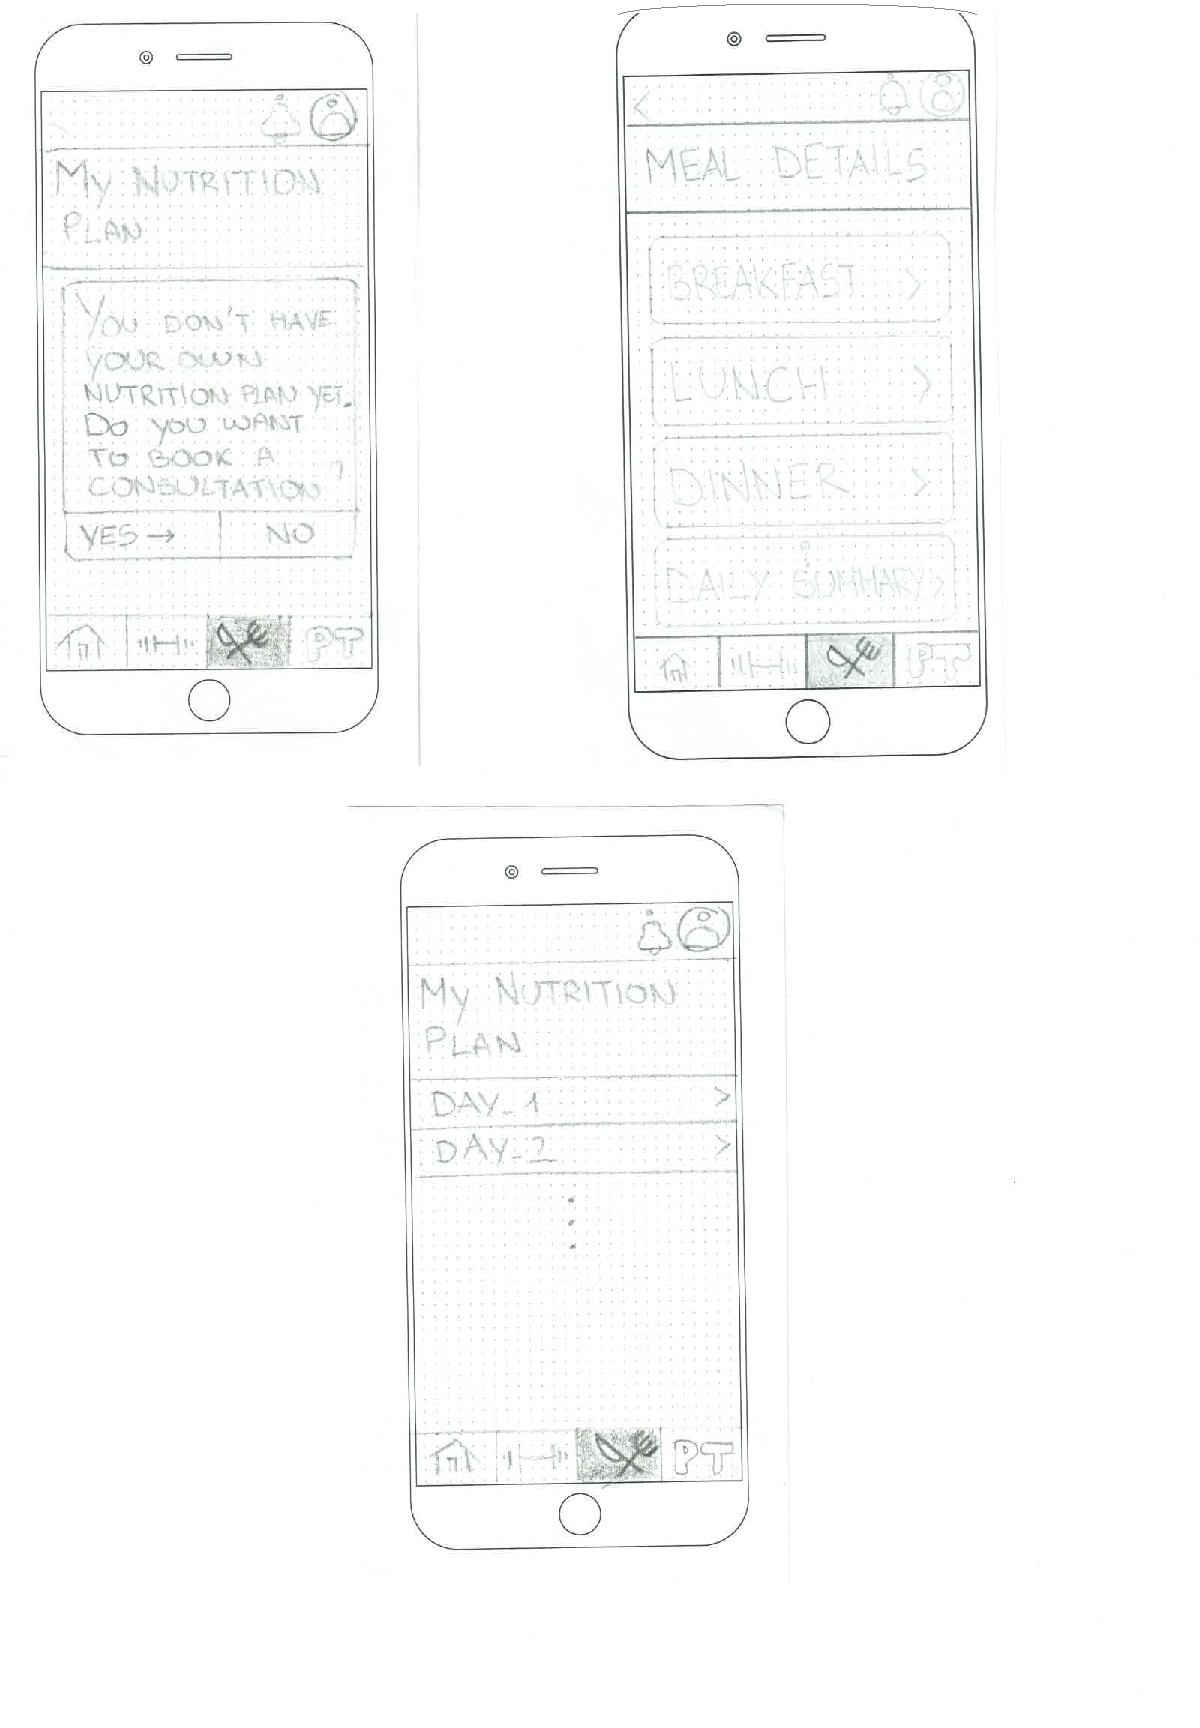
\includegraphics[width=0.80\textwidth]{4-ApplicationDesign/img/PaperPrototype/paper-member-nutrition-clean.pdf}
    \caption{Nutrition plan and meal details.}
    \label{fig:paperMemberNutrition}
\end{figure}

\clearpage
\begin{figure}[H]
    \centering
    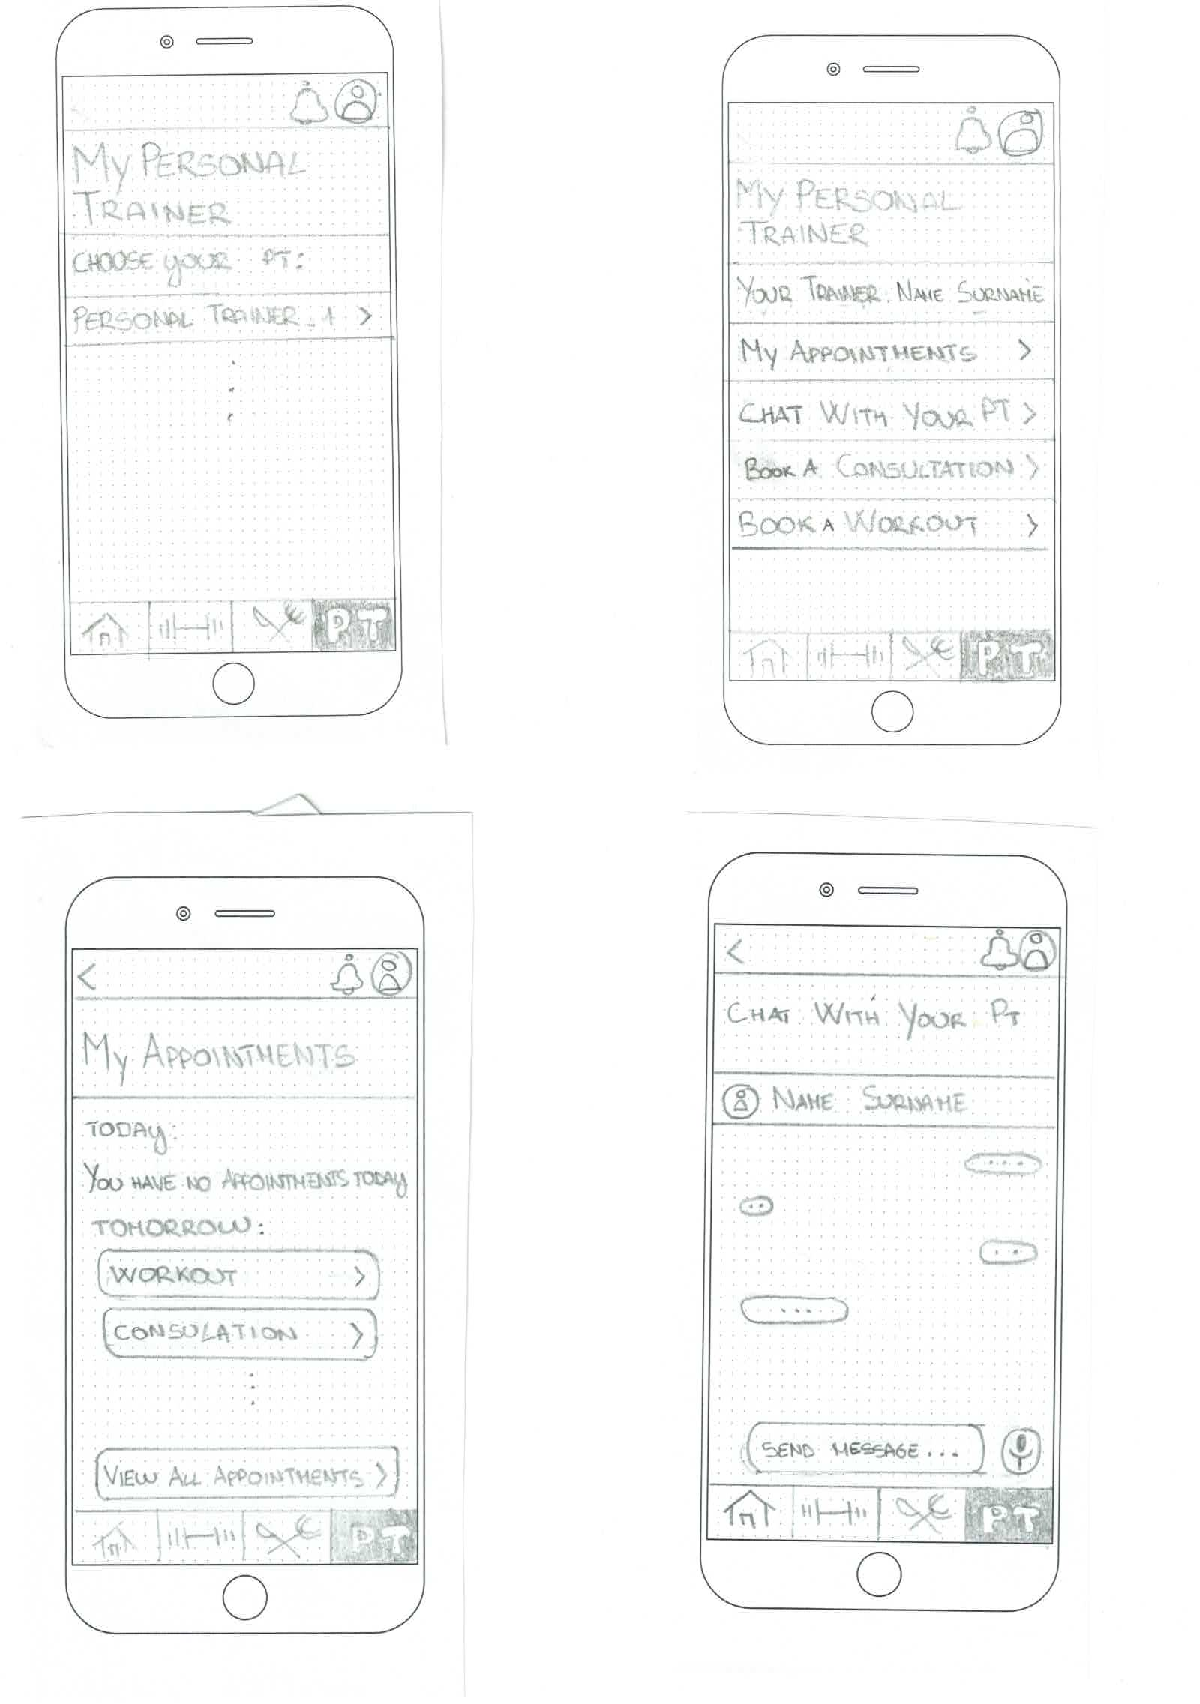
\includegraphics[width=0.80\textwidth]{4-ApplicationDesign/img/PaperPrototype/paper-member-trainer.pdf}
    \caption{Trainer selection, appointments, and chat.}
    \label{fig:paperMemberTrainer}
\end{figure}

\clearpage
\begin{figure}[H]
    \centering
    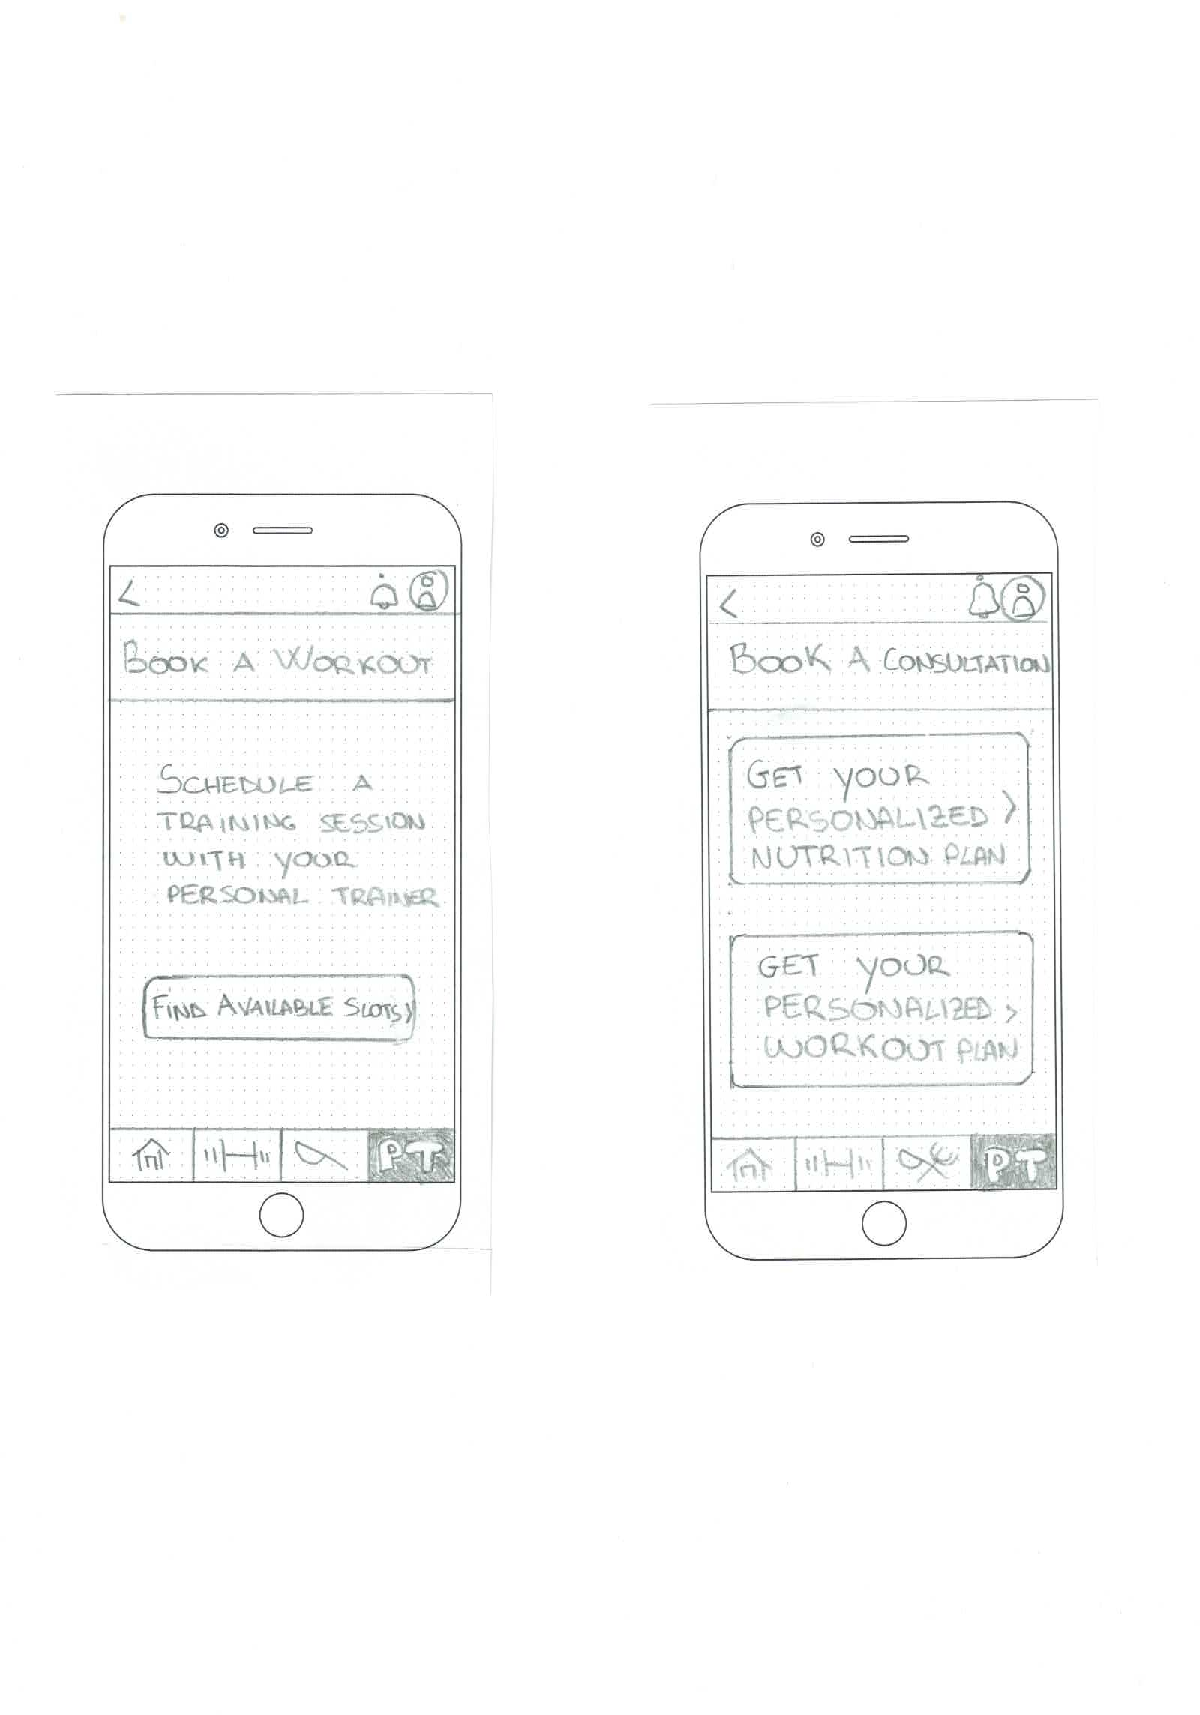
\includegraphics[width=0.72\textwidth,trim=18bp 175bp 34bp 165bp,clip]{4-ApplicationDesign/img/PaperPrototype/paper-member-booking.pdf}
    \caption{Booking entry points.}
    \label{fig:paperMemberBooking}
\end{figure}

\clearpage
\begin{figure}[H]
    \centering
    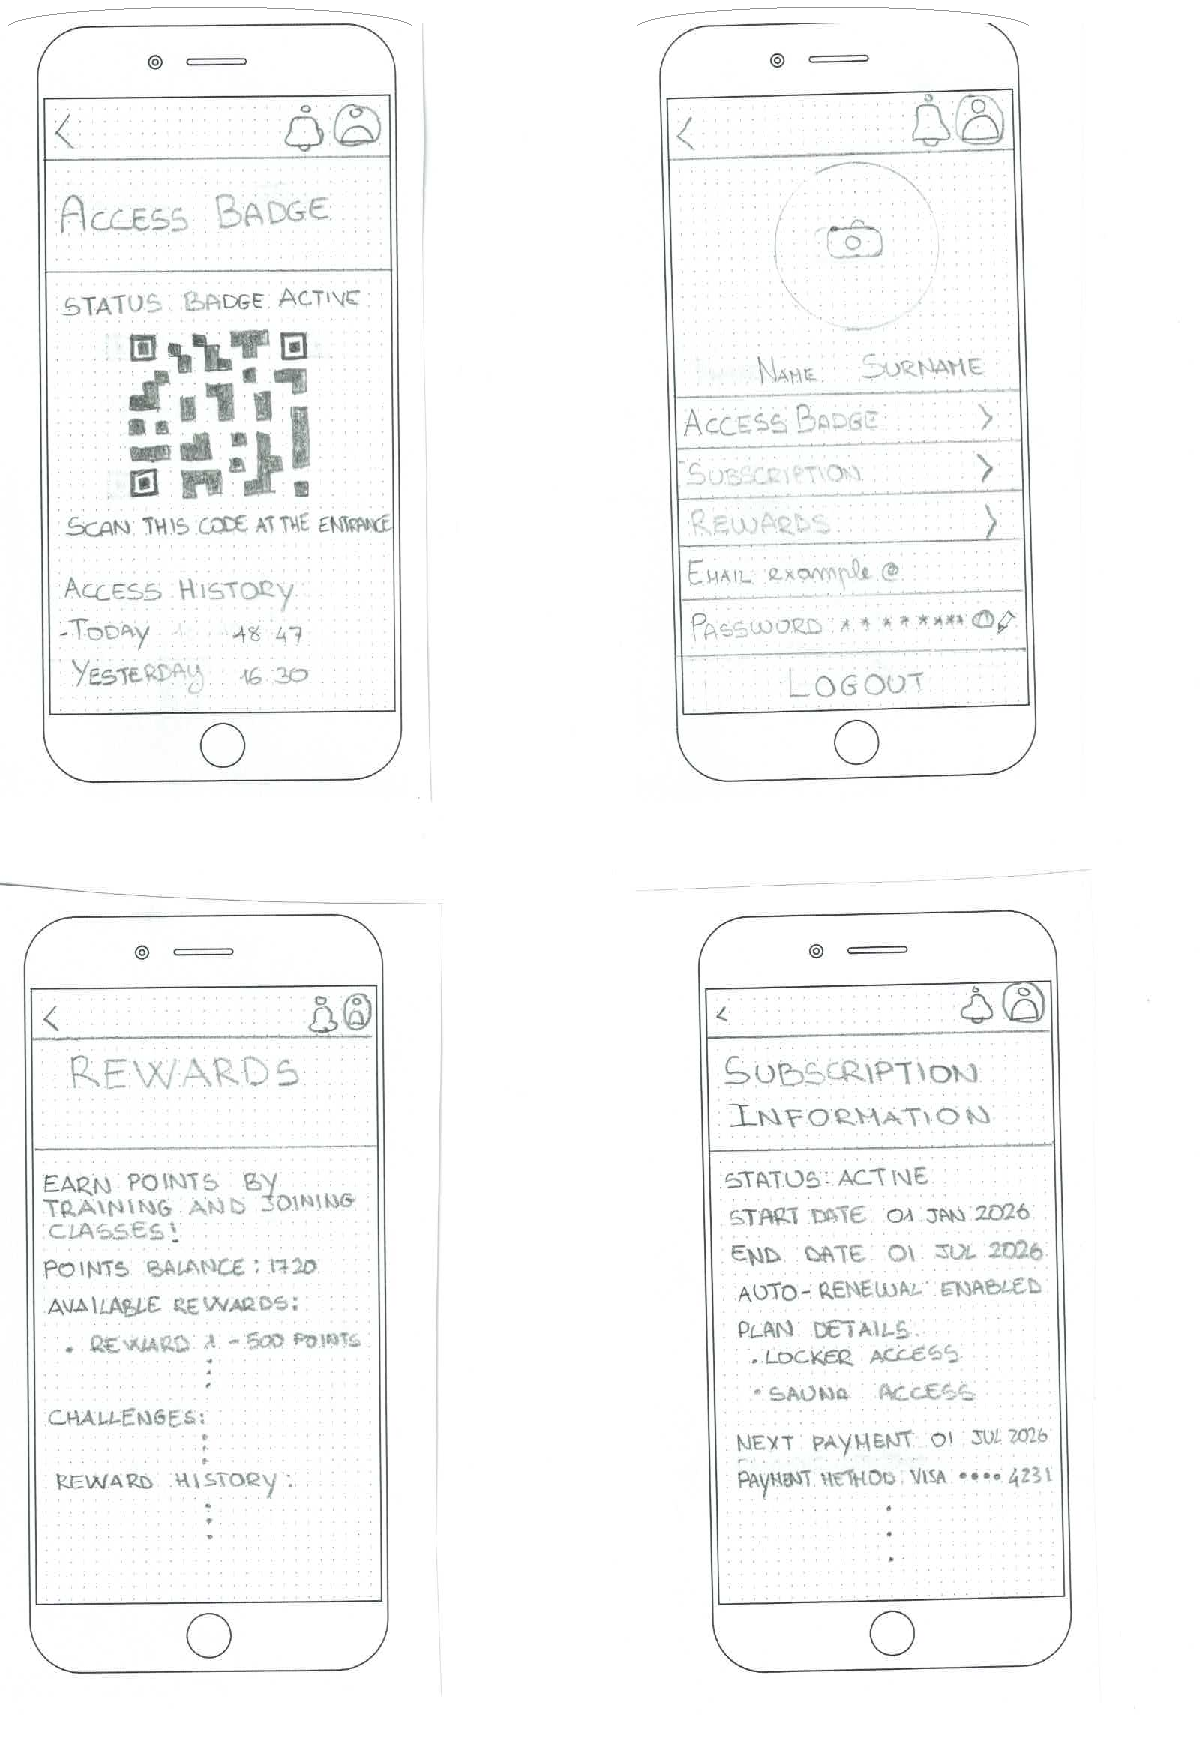
\includegraphics[width=0.80\textwidth]{4-ApplicationDesign/img/PaperPrototype/paper-member-profile-clean.pdf}
    \caption{Profile and membership.}
    \label{fig:paperMemberProfile}
\end{figure}

\clearpage
\paragraph{Professional Screens}

The professional sketches begin with the client list and use the selected client as the entry point for workout creation, nutrition management, progress, and appointments (Figure \ref{fig:paperProfessionalClients}). Profile, chat, and calendar remain independent destinations in the professional navigation (Figure \ref{fig:paperProfessionalScreens}).

\begin{figure}[H]
    \centering
    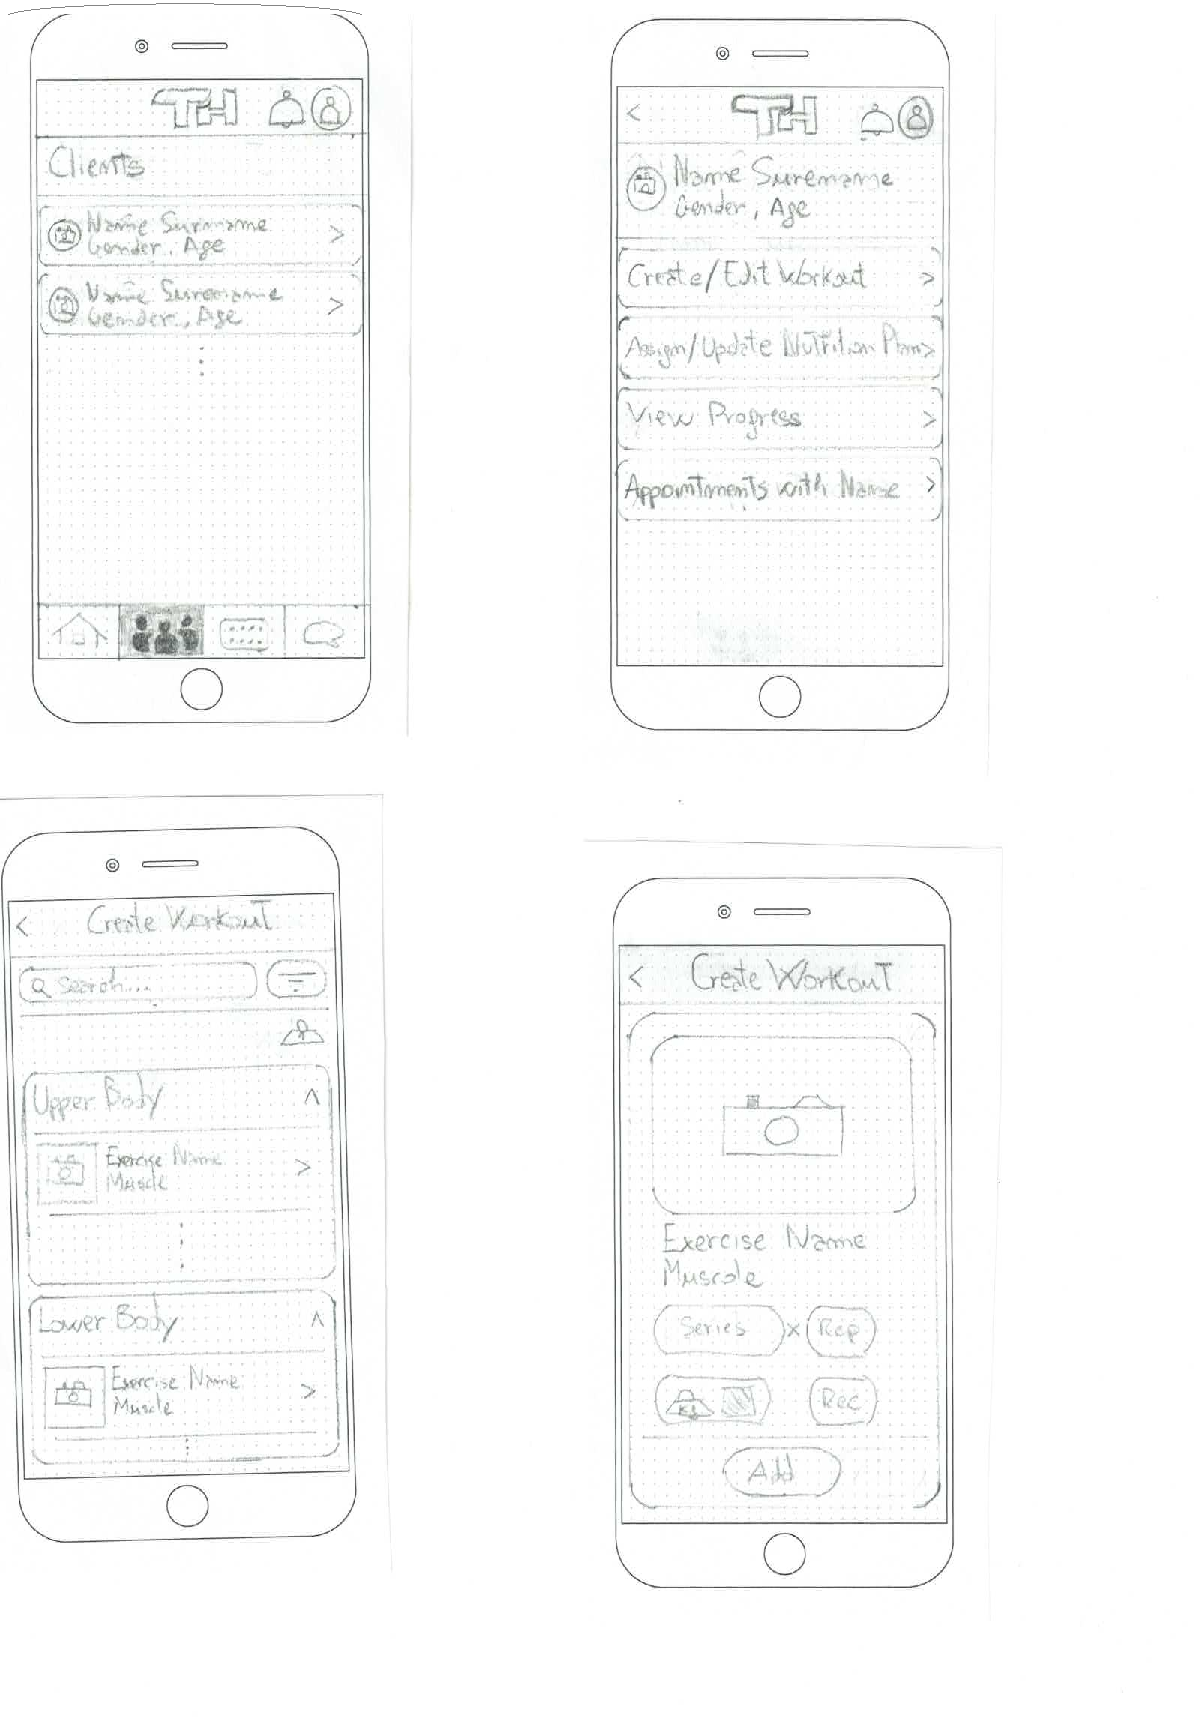
\includegraphics[width=0.56\textwidth]{4-ApplicationDesign/img/PaperPrototype/paper-professional-clients-clean.pdf}
    \caption{Client management and plan creation.}
    \label{fig:paperProfessionalClients}
\end{figure}

\clearpage
\begin{figure}[H]
    \centering
    \begin{subfigure}[b]{0.31\textwidth}
        \centering
        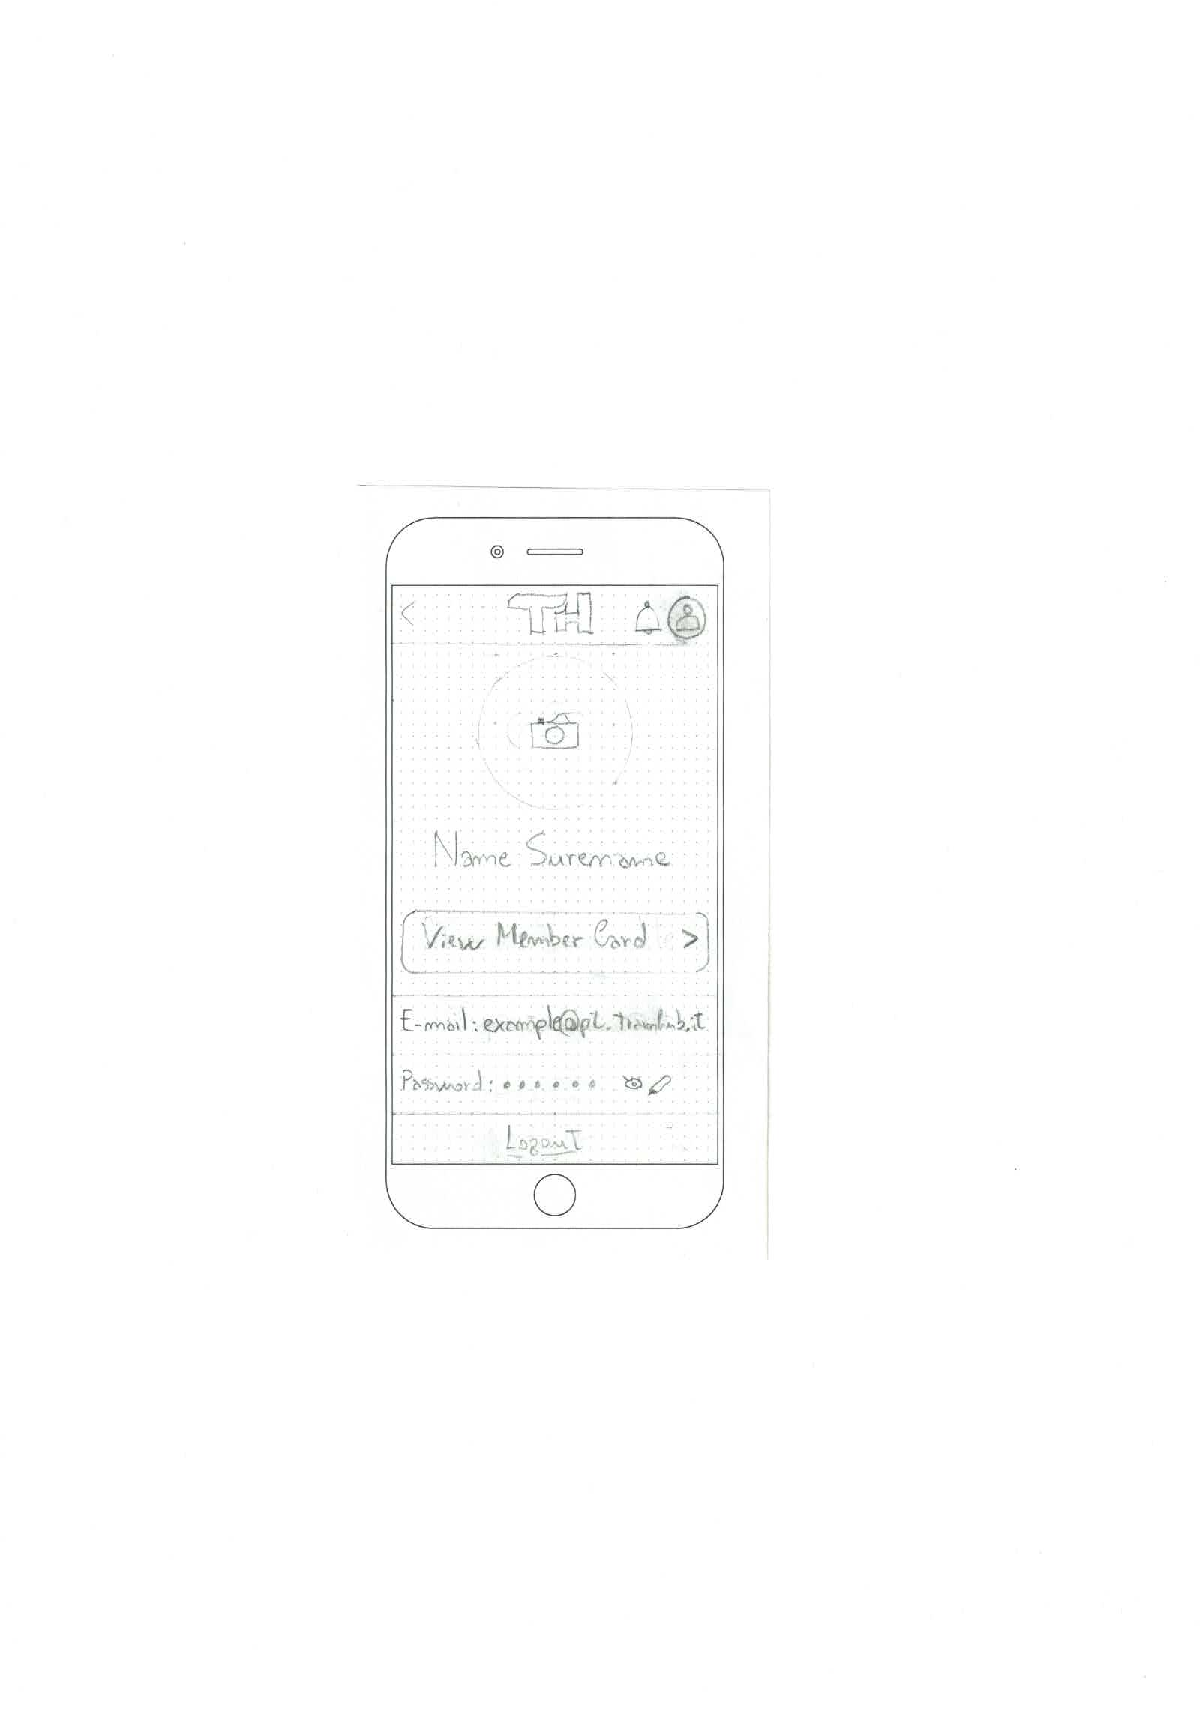
\includegraphics[height=7.5cm,keepaspectratio,trim=150bp 195bp 180bp 185bp,clip]{4-ApplicationDesign/img/PaperPrototype/paper-professional-profile.pdf}
        \caption{Profile.}
    \end{subfigure}
    \hfill
    \begin{subfigure}[b]{0.31\textwidth}
        \centering
        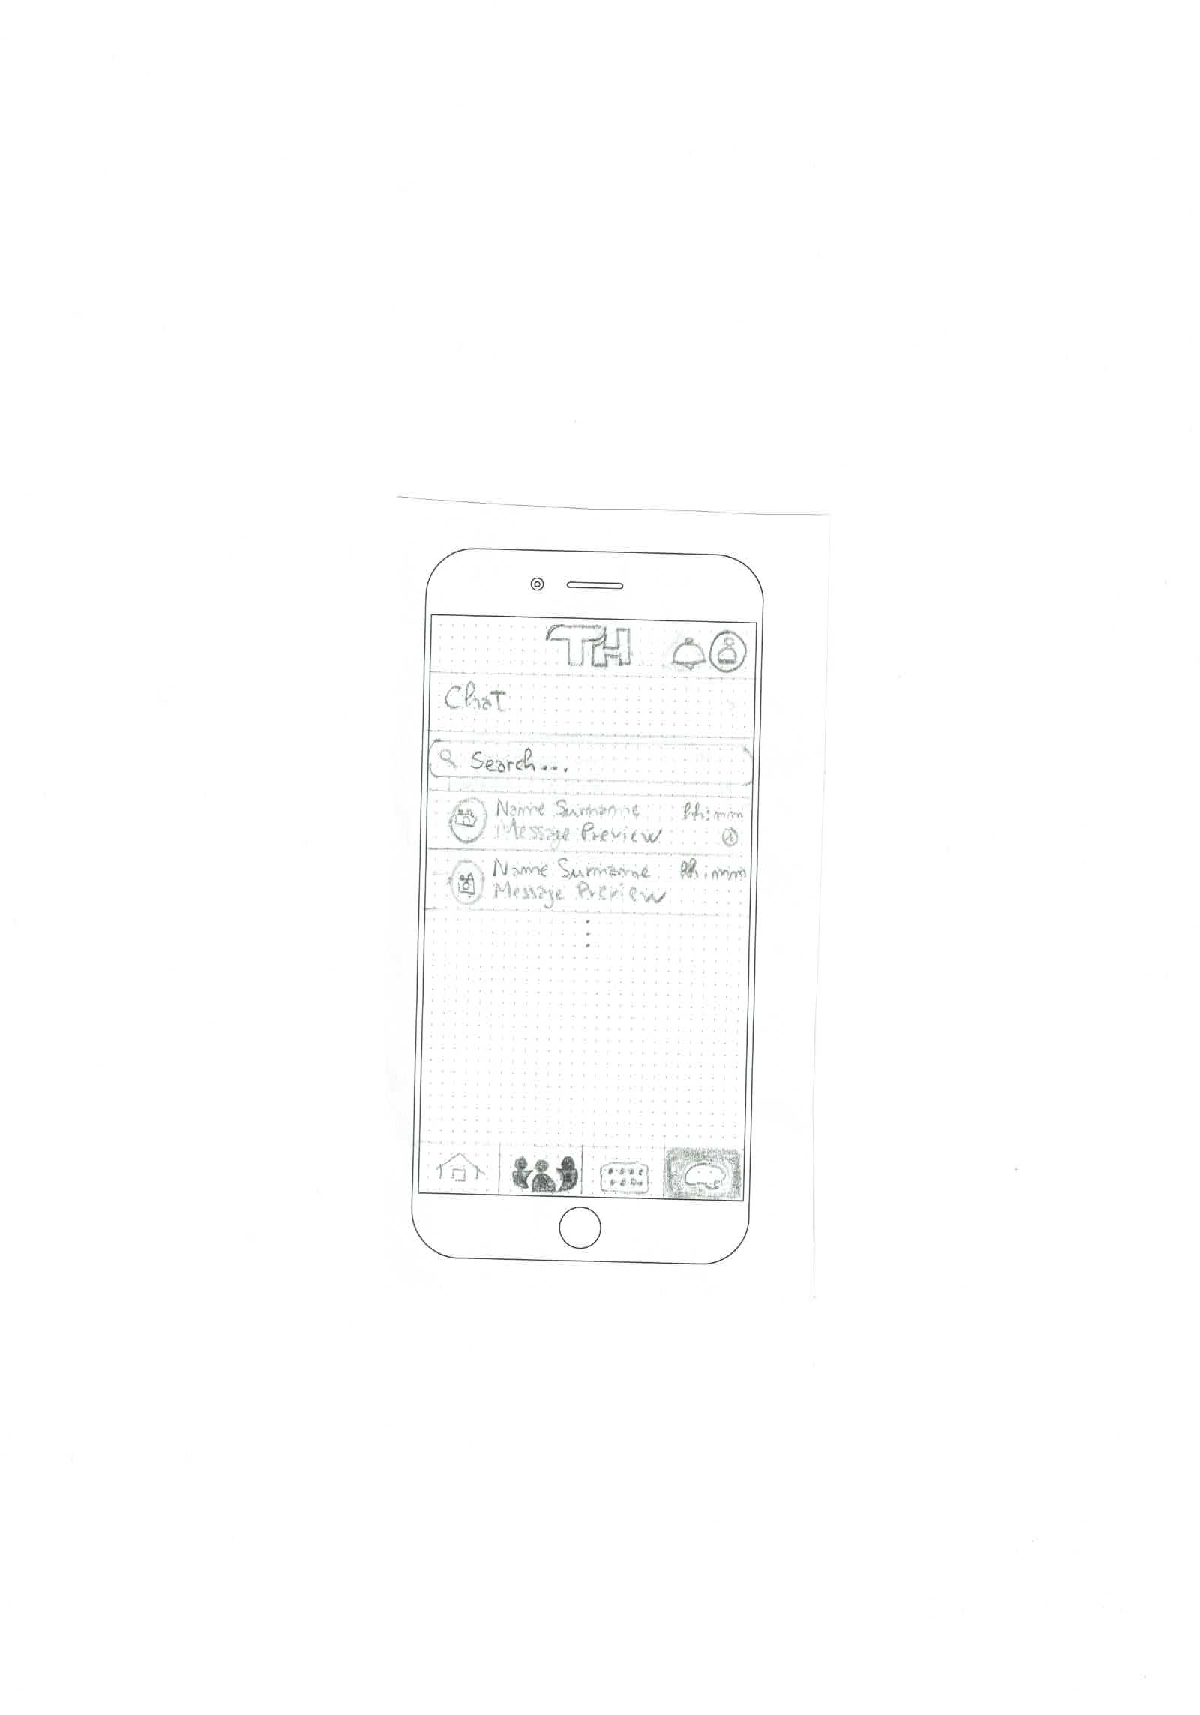
\includegraphics[height=7.5cm,keepaspectratio,trim=165bp 185bp 155bp 195bp,clip]{4-ApplicationDesign/img/PaperPrototype/paper-professional-chat.pdf}
        \caption{Chat.}
    \end{subfigure}
    \hfill
    \begin{subfigure}[b]{0.31\textwidth}
        \centering
        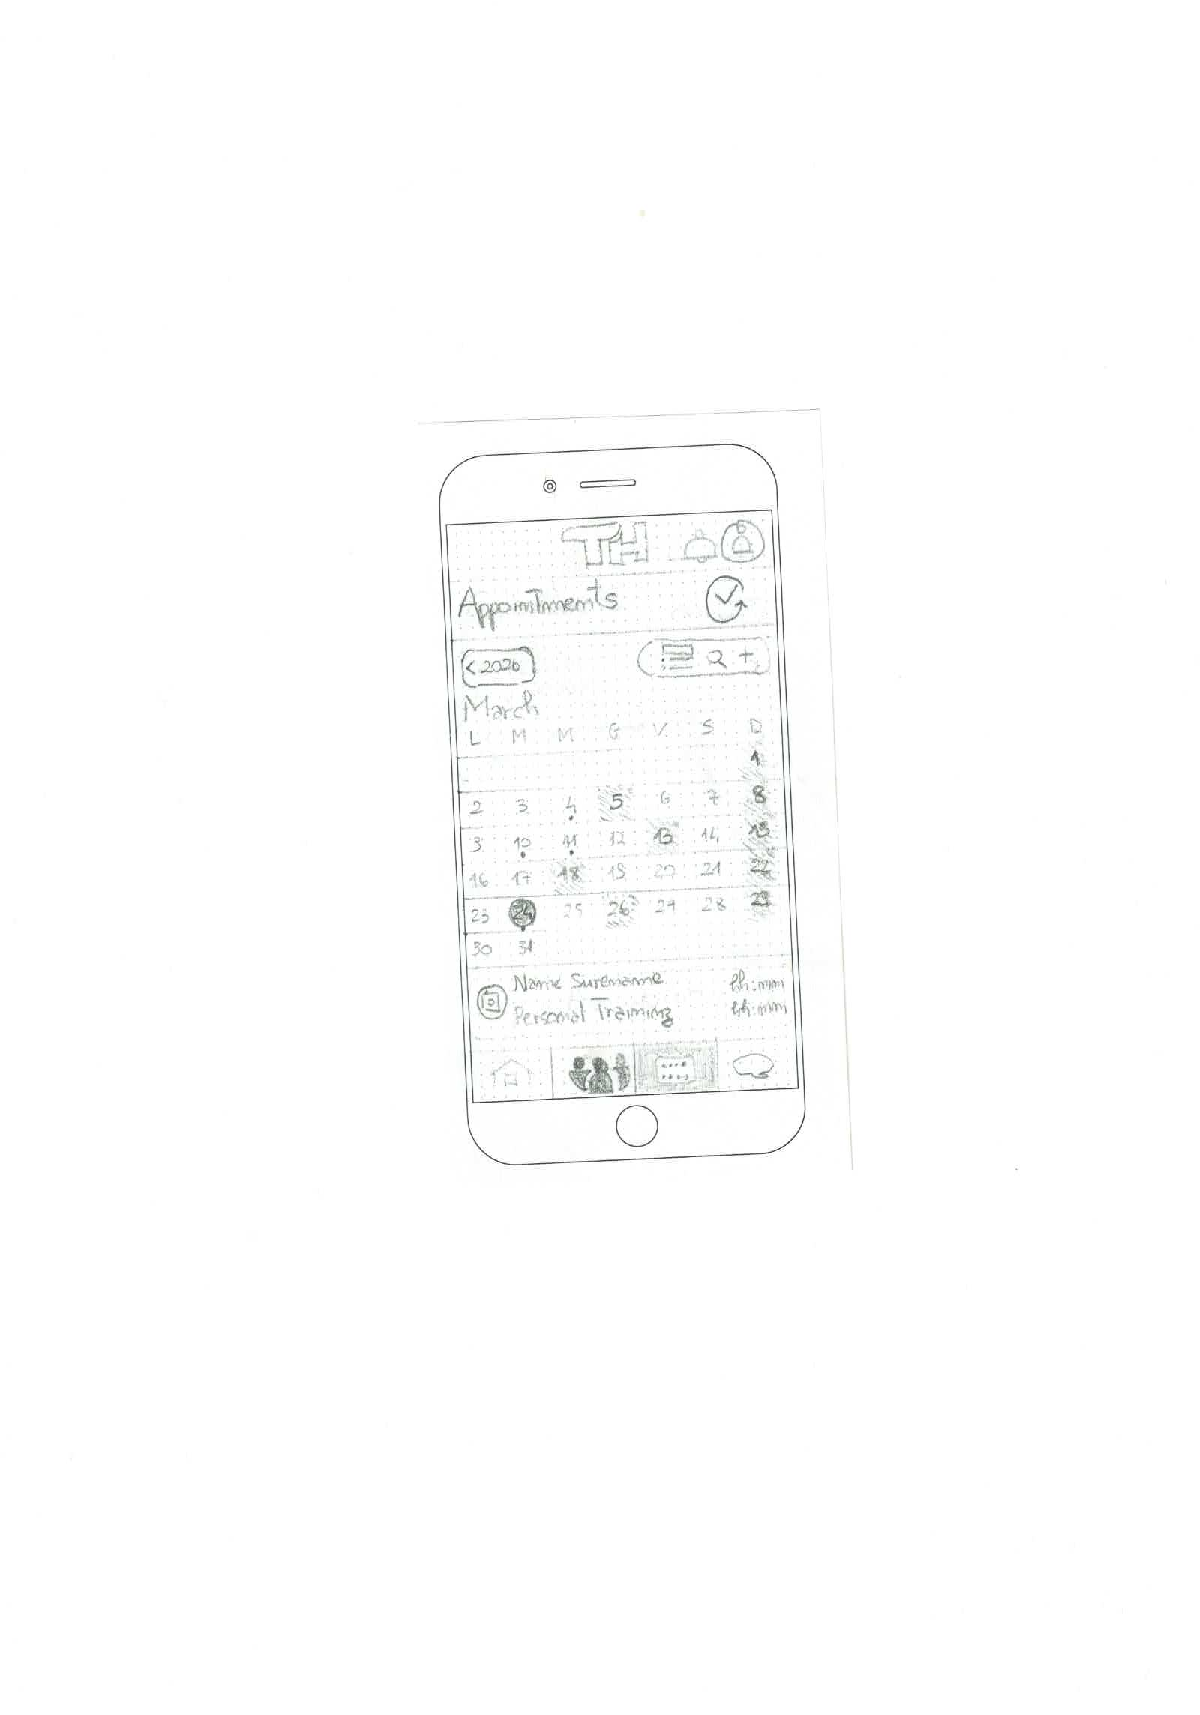
\includegraphics[height=7.5cm,keepaspectratio,trim=150bp 190bp 140bp 165bp,clip]{4-ApplicationDesign/img/PaperPrototype/paper-professional-calendar.pdf}
        \caption{Calendar.}
    \end{subfigure}
    \caption{The professional's independent destinations in the paper prototype.}
    \label{fig:paperProfessionalScreens}
\end{figure}

\clearpage

\subsection{Digital Prototype}\label{subsect:DigitalPrototype}
% Link o QR code al progetto Figma interattivo (sul modello del QR code in
% Hammami_Hub, fig. 3.1). Intro breve: da qui in poi i mockup digitali sono
% raggruppati per flusso (non una schermata per sottosezione), sul modello di
% BookIT 4.4 / Hammami_Hub 3.4 -- ogni flusso ha gli screenshot delle
% schermate coinvolte in sequenza, e un diagramma mermaid a frecce quando il
% flusso dirama (piu' di un percorso possibile) o le transizioni non sono
% ovvie dal solo screenshot. Tre gruppi: comuni ai due ruoli, poi cliente,
% poi professionista.

\paragraph{Common Flows}

\subsubsection{Login \& Reset Password Flow}\label{subsubsect:LoginResetFlow}
% Login -> Forgot Password -> Reset Password, piu' il redirect post-login al
% ruolo corretto (/m o /p, in base al profilo). Wireframe esistenti solo in
% doc/assets/pt/01-03 (Login, Forgot Password, Set Password) -- condivisi tra
% i due ruoli, nessun set separato lato cliente. Diagramma mermaid lineare,
% con un ramo per "password dimenticata" e uno per il login diretto.

\subsubsection{Plan Creation \& Editing Flow}\label{subsubsect:PlanCreationEditingFlow}
% CreatePlanFlow.jsx e' condiviso testualmente tra i due ruoli ("Used by both
% roles. Only memberId, authorId and onDone differ.") -- un solo flusso, non
% duplicato. Ramo principale: 2 step in-pagina (nome piano -> prima sessione
% con esercizi aggiunti via autocomplete inline), nessuna schermata di
% riepilogo -- torna dritto alla panoramica del piano. Entry point diverso
% per ruolo: tab Workout per il cliente, Client Detail per il professionista
% -- da annotare nel diagramma, non da raccontare due volte.
%
% Ramo secondario, editing di un piano gia' esistente (aggiungere una
% sessione o un esercizio): stesso SessionForm, ma interfaccia diversa per
% ruolo -- lato cliente sono due schermate a parte (Add a Session, Add an
% Exercise), lato professionista e' tutto inline dentro Client Detail /
% Workout Plan (nessuna navigazione). Il diagramma deve mostrare questa
% divergenza, non solo il ramo comune.

\paragraph{Client Flows}

\subsubsection{Home \& Global Navigation Flow}\label{subsubsect:ClientHomeNavFlow}
% Home come screenshot d'apertura della sezione Cliente. Frecce etichettate
% "tab bar" verso Workout, Nutrition, My Trainer; freccia etichettata
% "avatar" verso Profile. Sono i punti d'accesso sempre raggiunti dalla shell
% dell'app (bottom nav + top bar), non link dentro il contenuto della Home --
% da leggere come premessa visiva ai flussi seguenti, non come schermata con
% link propri.

\subsubsection{Workout Plan Exploration Flow}\label{subsubsect:WorkoutExplorationFlow}
% Workout Plan -> Session Detail -> Exercise Detail, senza avviare una
% sessione live. Percorso di sola consultazione.

\subsubsection{Live Session Flow}\label{subsubsect:LiveSessionFlow}
% Session Detail -> Live Session -> Exercise Detail Live (stato inline dentro
% Live Session, non una route separata) -> Open-Run Sheet / End-Run Sheet
% (overlay) -> Congratulations Dialog (overlay) -> Session Summary. Diagramma
% mermaid con frecce per le diramazioni: Open-Run Sheet quando un secondo run
% si apre mentre uno e' gia' attivo, "Stopped Early" quando si esce da
% End-Run Sheet senza completare.

\subsubsection{Nutrition Flow}\label{subsubsect:NutritionFlow}
% Nutrition Plan -> Meal Detail (route /m/nutrition/meal/:mealId gia'
% esistente, wireframe ancora da fare -- nodo comunque presente, non
% taciuto). Ramo stato vuoto (nessun piano assegnato) -> Book Appointment,
% che rimanda al Personal Trainer \& Booking Flow.

\subsubsection{Personal Trainer \& Booking Flow}\label{subsubsect:TrainerBookingFlow}
% My Trainer -> Chat; My Trainer -> View Appointments -> Booking Sheet ->
% conferma prenotazione. Ramo "nessun professionista assegnato" -> Browse
% Trainers (redirect automatico da My Trainer quando non c'e' ancora un
% professionista scelto).

\subsubsection{Profile Flow}\label{subsubsect:ClientProfileFlow}
% Profile -> Access Badge, Subscription, Rewards, Settings. Diagramma a
% stella: tutti i rami partono da Profile, nessun collegamento tra loro.

\paragraph{Professional Flows}

\subsubsection{Home \& Global Navigation Flow}\label{subsubsect:ProHomeNavFlow}
% Stessa struttura del flusso Home lato cliente: Home come screenshot
% d'apertura, frecce "tab bar" verso Clients, Calendar, Chat; freccia
% "avatar" verso Profile. L'agenda mostrata in Home include anche
% un'anteprima appuntamenti che rimanda al Calendar Flow -- non ripetuta qui,
% solo richiamata.

\subsubsection{Calendar Flow}\label{subsubsect:CalendarFlow}
% Calendar -> Availability. Calendar -> Appointment Detail (raggiungibile
% anche dall'anteprima appuntamenti in Home). Nuovo appuntamento ("+") come
% azione inline sulla stessa schermata di Calendar, non una route a parte.

\subsubsection{Client Management Flow}\label{subsubsect:ClientManagementFlow}
% Clients -> Client Detail -> quattro rami: Chat (stesso nodo Chat della tab
% bar -- doppia via d'accesso, un solo screenshot di destinazione); Workout
% Plan (rimanda al Plan Creation \& Editing Flow comune, meccanismo identico
% a quello del cliente); Nutrition Plan (consultazione + creazione/editing
% inline -- ramo professionista-only, il cliente non ha mai un bottone "+"
% qui); Progress Tracking (sola consultazione, nessuna creazione).

\subsubsection{Profile \& Settings Flow}\label{subsubsect:ProProfileSettingsFlow}
% Profile -> Settings. Molto piu' corto della versione cliente: nessun badge,
% subscription o rewards lato professionista.

\subsection{Visual Design}\label{subsect:VisualDesign}

The visual design follows the component sheet created in Figma. Inter is used as the primary typeface, with a clear distinction between page titles, section titles, body content, and secondary labels. Cards use generous rounded corners and light borders, while primary actions use a pill shape. Status information is never conveyed only by color: labels, icons, and progress values provide the same meaning in text.

The palette is stored as design tokens rather than repeated manually across screens. The main brand color is \texttt{\#FE6363}, the application background is \texttt{\#F9FAFB}, and additional semantic tokens represent success, warning, danger, text, borders, and appointment categories. The same token file used by the Figma project is imported by the application theme, reducing the possibility of the prototype and implementation drifting apart.

Material UI's \texttt{createTheme} function defines typography, spacing, shape, palette, and component overrides in one location. Responsive font sizing is then applied so headings adapt across mobile and wider layouts. Appointment cards use an additional semantic palette group, \texttt{palette.task}, with one entry per appointment kind and per terminal state: training, protocol, nutrition, done, and suspended. The first four come from the token file's task group and the last from its status group, so a card's colour is decided in Figma and read in the theme rather than chosen again in the component. All screen-level styling is expressed through Material UI and the theme rather than through separate CSS files.

The final interface preserves the soft cards and compact navigation of the prototype while improving clarity in nested pages. Shared page headers provide a consistent back action, sticky top and bottom regions keep global navigation available, and forms place validation or offline information next to the action it affects. Notification filters and selection states use labels and checkboxes in addition to color, while the membership banner keeps an account-wide restriction visible without hiding the page underneath it.

\subsection{Deviations from the Wireframes}\label{subsect:Deviations}

The prototype remained the visual reference during implementation. Some changes became necessary after connecting the screens to real data and testing them on mobile devices.

\begin{itemize}
    \item \textbf{One professional role:} the early material described Personal Trainers, nutritionists, and dietitians as separate administrative experiences. The implementation uses one professional role with a specialty. This keeps one interface and enables or hides actions according to the professional's profile;
    \item \textbf{Profile access:} Profile was moved from the bottom navigation to the avatar in the top bar. This leaves four primary destinations per role and avoids an overcrowded navigation bar;
    \item \textbf{Contextual booking:} appointment creation is presented in a bottom sheet rather than as a separate route. The selected professional and day remain visible in the background, reducing the risk of losing context;
    \item \textbf{Data-backed information:} fields that do not exist in the database are not invented for presentation. The professional biography replaces the fixed experience value from the prototype, and the membership identifier is derived from the user's real profile identifier;
    \item \textbf{Access scanner:} the professional QR scanner and its top-bar entry point were added after the first wireframes. They are required to validate the rotating badge designed for the member;
    \item \textbf{Weekly workout runs:} the original live-session wireframes represented a workout that could be completed once. The implemented design records a new run whenever a session is trained, derives progress from the current week, and preserves previous results. It also adds a persistent mini-player, end-of-run confirmation, and a run-specific summary;
    \item \textbf{Draft-then-commit plan creation:} the initial workout form created only one session before returning to the plan. The final wizard keeps any number of sessions in a local draft, adds a review step, and writes the complete plan only after confirmation. The nutrition editor follows the same pattern with day types and meals;
    \item \textbf{Workout-plan history:} editing produces a replacement plan instead of deleting or overwriting prescriptions already referenced by completed workouts. The latest version is shown as active, while previous versions remain available to the database history;
    \item \textbf{Nutrition day types:} the prototype showed the same meals independently of the selected date. The implemented plan assigns reusable day types to weekdays, so the week selector now changes the meals displayed and each meal can include macronutrients and alternatives;
    \item \textbf{No PDF export of the nutrition plan:} the prototype's client screen offered a \textit{View Full PDF Plan} action beside the assigned diet. The implemented plan is structured data the application reads directly, so a generated document would be a second copy of the same information, free to drift from the rows once a day type or a meal is corrected, and it would require file storage the project does not otherwise need. The plan is therefore consulted in the interface, where it is always the current version;
    \item \textbf{Membership enforcement:} subscription status was originally presented as information. In the implemented flow it also controls access to booking, plan creation, gym entry, and reward earning. A professional can suspend or reactivate an assigned client, while the member receives a persistent explanation when services are paused;
    \item \textbf{Body measurements removed:} the progress area was designed around periodic body measurements entered by hand. Nothing in the application produced that data, and asking a professional to type it during a session was slower than the paper card it replaced. Progress now reports what the app actually records: weekly training, the detail of each run, and the member's closing note;
    \item \textbf{Exercise media:} the prototype's graphic exercise blocks were retained as placeholders. Producing and licensing a complete set of images or videos was outside the project scope, and using inconsistent external material would have reduced the visual coherence of the application.
\end{itemize}

These deviations preserve the purpose of the original screens while adapting them to the implemented flows.

A last group of changes came from the prototype being right on the artboard and wrong on the phone, which is worth recording because it is a limit of static prototyping rather than a design mistake. The empty circle drawn on appointment cards was meant as a quick "mark as done" control; that control was never built, and the circle survived as decoration that looks like a checkbox. The calendar was designed in a collapsed and an expanded state, which sit side by side in Figma but force the running application to open in whichever of the two is less useful. The row of dots representing the weekly goal is drawable for a fixed number of sessions and runs off the screen at six or more. None of the three is visible until the screen is real, on a real display, holding real data.


\newpage
\section{Implementation and Architecture}\label{sect:ImplementationArchitecture}

The implementation of TrainHub follows the distinction established during the design phase: members and professionals use different interfaces, but both work on the same information. A workout assigned by a trainer, a message sent in chat, or a confirmed appointment must be visible from the other side without creating separate copies of the data. For this reason, the application was developed as a single Progressive Web App connected to a shared backend.

This chapter focuses on the structure that supports the final interface. Rather than describing the screens again, it explains how navigation, local state, persistent data, offline behaviour, and device features cooperate during the main user flows.

\subsection{Technology Stack}\label{subsect:TechnologyStack}

TrainHub is a client-side web application built with React and Vite. React provides the component model used throughout the interface, while Vite manages the development environment and creates the optimized production bundle. Material UI supplies the component foundation and theme system, and React Router maps the two role-specific navigation trees described in Section \ref{subsect:NavigationMap}.

Supabase provides authentication, the PostgreSQL database, Realtime updates, and the server-side function used to deliver push notifications. TanStack Query sits between the interface and the data functions: it manages remote state, keeps query results synchronized, and persists the useful part of the cache in IndexedDB. The main technologies, the versions the delivered build was compiled against, and their role in the project are summarized in Table \ref{tab:technologyStack}.

\begin{table}[H]
    \centering
    \small
    \begin{tabularx}{\textwidth}{@{}p{0.22\textwidth} p{0.11\textwidth} >{\raggedright\arraybackslash}X@{}}
        \toprule
        \textbf{Technology} & \textbf{Version} & \textbf{Use in TrainHub} \\
        \midrule
        React & 19.2 & Component-based interface and the hooks that hold screen-local state \\
        Vite & 8.1 & Development server, production build, and route-level code splitting \\
        Material UI & 9.2 & Responsive components, shared visual rules, typography, and theme customization \\
        React Router & 8.3 & Public routes, protected member and professional areas, and route-level error handling \\
        TanStack Query & 5.101 & Loading and mutation state, cache invalidation, offline queues, and persisted server data \\
        Supabase JS & 2.110 & User sessions, PostgreSQL access, Realtime channels, and stored procedure calls \\
        vite-plugin-pwa & 1.3 & Manifest injection and the build step that lists the files to precache \\
        Workbox & 7.4 & Precaching and navigation routing inside the hand-written service worker \\
        \bottomrule
    \end{tabularx}
    \caption{Main technologies used in the final application.}
    \label{tab:technologyStack}
\end{table}

The application is written in JavaScript and JSX. Keeping one language across the interface and data-access layer made the project easier to inspect during development, while the database remains responsible for rules that cannot safely depend on the browser.

\subsection{Application Structure}\label{subsect:ApplicationStructure}

The source code is organized by responsibility and by feature. Shared building blocks remain separate from domain-specific screens, while calls to persistent data are collected in plain asynchronous functions. Table \ref{tab:sourceStructure} shows the main directories.

\begin{table}[H]
    \centering
    \small
    \begin{tabularx}{\textwidth}{@{}p{0.24\textwidth} >{\raggedright\arraybackslash}X@{}}
        \toprule
        \textbf{Directory} & \textbf{Responsibility} \\
        \midrule
        \path{src/routes} & Public routes and the protected member and professional route trees \\
        \path{src/layouts} & The signed-in application shell and the centred layout used by the authentication screens \\
        \path{src/features} & Screens and feature-specific components, one folder per domain: authentication, home, agenda, workout, nutrition, trainer, clients, calendar, chat, notifications, progress, rewards, check-in, and profile \\
        \path{src/components} & Reusable interface elements such as page headers, navigation controls, status feedback, and shared cards \\
        \path{src/data} & Database reads and writes, grouped by application domain and independent from React \\
        \path{src/lib} & Supabase configuration, query keys, cache persistence, date utilities, identifiers, and other shared services \\
        \path{src/theme} & Material UI theme and the visual tokens exported from the Figma design \\
        \bottomrule
    \end{tabularx}
    \caption{Responsibilities of the main source directories.}
    \label{tab:sourceStructure}
\end{table}

The dependency direction is deliberately one-way. Modules in \path{src/data} know about Supabase and nothing about React; modules in \path{src/features} know about React and call \path{src/data}; components know about neither and render what they are given. A pure module such as the week calculation in \path{src/lib} can therefore be used by a data function and by a screen at the same time, which would not be possible if the shared code lived beside the screens that first needed it.

This organization also avoids placing database details inside every screen. A page requests the information it needs through a query, and the corresponding function in \path{src/data} translates that request into a Supabase operation. The same functions can therefore be used from different screens without duplicating filters, date conversions, or error handling. Authentication and Realtime subscriptions are the main exceptions: they are tied to the browser session and the component life cycle, so they remain close to the providers and hooks that own them.

\subsubsection{Application Shell and Routing}\label{subsubsect:ApplicationShellRouting}

At start-up, the root component installs the Material UI theme, the persisted query client, the authentication provider, and the router. The authentication provider first restores the Supabase session and then loads the associated profile. The profile identifies the user's role and assigned professional, information that is required by most protected flows.

Member routes use the \path{/m} prefix and professional routes use \path{/p}. The guard is the shell itself: each protected tree declares the role it expects, so a signed-in user who opens the other area is redirected to their own home page, while a visitor who is not signed in is sent to the login screen with the requested address remembered for after. Both trees are rendered inside that same shell, which contains the top bar, bottom navigation, offline feedback, membership banner, notification status, and the mini-player shown during an open workout. Screen modules are loaded only when their route is visited, so each section ships as its own chunk and the first view downloads a fraction of the application.

Detail pages return to their parent section through one shared header rather than through a back arrow drawn per screen, so a link opened from a notification still lands on a complete page with a valid way out. Unexpected route errors are handled by a shared error screen instead of leaving the application blank.

\subsubsection{Remote State and Mutations}\label{subsubsect:RemoteStateMutations}

Information read from Supabase is treated as remote state. Every query uses a shared key that identifies both the domain and the relevant user or record. When an operation changes data, related keys are invalidated together so that all affected views are refreshed. For example, completing a workout updates the current run, the weekly workout summary, the rewards area, and the professional's progress view without requiring those screens to know about each other.

Two defaults shape the whole offline behaviour, and they are set once for every query in the application.

\begin{lstlisting}[language=JavaScript,caption={Query defaults, in \texttt{src/lib/queryClient.js}.},label={lst:queryDefaults}]
queries: {
  gcTime: ONE_WEEK,
  staleTime: 1000 * 30,
  // Retrying while offline pauses the query instead of failing it, so
  // `isPending` would stay true forever and no screen could ever show
  // its offline state.
  retry: (failureCount) => navigator.onLine && failureCount < 2,
  refetchOnWindowFocus: false,
  // Serve cached data immediately and only then reach for the network.
  networkMode: 'offlineFirst',
}
\end{lstlisting}

The consequence is that a failed refresh is not the same as an absent answer. Screens decide their error state on whether data exists at all, never on the failure of the last request: an error page drawn over perfectly usable cached data would tell an offline member that the application is broken while it is doing exactly what it was built to do.

Writes follow the same pattern, but they need one thing more. The function a write executes is registered centrally, before the persisted cache is restored, rather than being passed at the call site. This matters for an offline mutation: after the application has been closed and reopened, the stored operation is found again by its key, and a restored write with no registered function is discarded without a message. Operations whose order matters share a scope, because paused writes are otherwise replayed in parallel and a set could reach the database before the run it belongs to.

\begin{lstlisting}[language=JavaScript,caption={A registered write, with the scope that keeps the workout writes in order.},label={lst:mutationDefault}]
queryClient.setMutationDefaults(mutationKeys.resumeRun, {
  mutationFn: resumeRun,
  onSuccess: (data, variables) => { /* update the open run in cache */ },
  scope: runScope,
  onSettled: () => {
    queryClient.invalidateQueries({ queryKey: queryPrefixes.runs })
  },
})
\end{lstlisting}

Some immediate actions are deliberately excluded from this queue. A badge token that expires after a minute, the redemption of a gym entry, and the registration of a push subscription cannot represent a real event if they are replayed much later. When the device is offline, these actions fail immediately and the interface explains that a connection is required.

\subsection{Backend and Data Model}\label{subsect:BackendDataModel}

The backend uses a relational PostgreSQL schema of twenty-one tables, because the principal entities are strongly connected. A member belongs to a professional, a plan contains sessions, a session contains exercises, and every completed set belongs to one specific workout run. Preserving these relations in the database makes it possible to enforce ownership and consistency independently of the interface.

The data model can be divided into the areas shown in Table \ref{tab:dataAreas}.

\begin{table}[H]
    \centering
    \small
    \begin{tabularx}{\textwidth}{@{}p{0.26\textwidth} >{\raggedright\arraybackslash}X@{}}
        \toprule
        \textbf{Area} & \textbf{Stored information} \\
        \midrule
        Accounts & Profiles, roles, professional assignment, specialty, and membership status \\
        Workouts & Exercise catalogue, versioned plans, sessions, prescribed exercises, workout runs, individual set logs, and rewards \\
        Nutrition & Versioned plans, reusable day types assigned to weekdays, and meals with their macronutrients \\
        Organization & Professional availability, appointment requests, confirmations, and cancellations \\
        Communication & One member--professional thread, messages, read receipts, and persistent notifications \\
        Facility access & Short-lived badge tokens and recorded check-ins \\
        Devices and configuration & Registered push endpoints and the server-side settings used to deliver them \\
        \bottomrule
    \end{tabularx}
    \caption{Main areas of the TrainHub data model.}
    \label{tab:dataAreas}
\end{table}

The schema is relational with one deliberate exception: the foods inside a meal are stored as a JSON document rather than as a further table. They are never queried on their own, never referenced from elsewhere, and are always read and written together with the meal that contains them, so a fourth level of joins would have bought nothing.

Workout and nutrition plans are not overwritten when they are edited. The replacement records a link to the plan it supersedes, and a partial unique index allows any plan to be superseded only once, while workout runs continue to reference the plan and session that were actually used. This prevents a later change to the programme from rewriting the meaning of an older result. The current plan is simply the most recent one created for that member.

A similar distinction is used between a workout session and a workout run. The session describes what should be performed; the run records one attempt, including start time, pauses, logged sets, final percentage, outcome, and the member's closing note. Weekly progress is derived from these runs rather than stored as a permanent status on the session, so the same session can be trained more than once and a partial attempt remains different from a completed one. The session table still carries the status column of the earlier design; nothing reads it and nothing decides on it, and it was left in place because dropping a column is a destructive migration that would have bought only tidiness.

\subsubsection{Authorization and Consistent Writes}\label{subsubsect:AuthorizationConsistentWrites}

The browser connects to Supabase with the publishable project key. That key is compiled into the JavaScript bundle and is public by construction: it identifies the project and grants nothing on its own. Every request carries the authenticated user identity, and PostgreSQL answers it in two stages that are easy to confuse. It first checks the table privileges, and only then evaluates the Row Level Security policies. A table with impeccable policies and no privilege answers \texttt{permission denied} to everybody, while a policy whose condition never mentions the current user identity is readable by anyone holding the key. Both failures are silent from the application's point of view, and an early version of this project shipped the second one.

The rule that separates a member from a professional is written once and reused by every policy that needs it.

\begin{lstlisting}[language=SQL,caption={The predicate that encodes ownership, and one of the policies built on it.},label={lst:ownsMember}]
create function owns_member(target uuid) returns boolean
language sql security definer stable set search_path = '' as $$
  select target = auth.uid()
      or exists (
           select 1 from public.profiles
           where id = target and assigned_pro_id = auth.uid()
         );
$$;

create policy workout_runs_select on workout_runs
  for select using (owns_member(member_id));
\end{lstlisting}

The empty search path is a security measure rather than a formality: inside a function that runs with the definer's privileges, an unqualified table name would be resolved against the caller's temporary schema first, and a signed-in user controls that schema. One table, holding the settings used to deliver notifications, has neither a policy nor a privilege and is reachable only from inside the database.

Simple operations are protected by these policies alone. Everything that changes data goes through stored procedures instead, and the direct write privileges on those tables were revoked. Creating a workout plan inserts the plan, every drafted session, and all their exercises as a single transaction. Closing a workout computes the result from the sets that were actually logged and writes the reward in the same operation. If any part fails, the database is not left holding half a plan or a summary that describes work nobody did.

Client-generated identifiers make an exact retry safe after a lost connection: the second attempt lands on the same row instead of creating a second one. The same procedures compare the content behind a reused identifier and reject a collision rather than accepting it silently. Plan creation carries one further check: the caller sends the identifier of the version it believes it is replacing, and the database refuses the write if a newer plan has appeared in the meantime, so a member and their professional editing at the same time cannot overwrite each other unnoticed.

Membership rules are enforced at this level as well as in the interface. An inactive member cannot create a plan, request an appointment, enter through the QR badge, or earn a workout reward, although the run itself is still recorded. A professional may change the status only for a client assigned to them. Keeping these checks in the backend prevents a modified browser request from bypassing the disabled buttons shown on screen.

\subsection{Progressive Web App and Offline Behaviour}\label{subsect:PWAOffline}

TrainHub includes a web app manifest with its name, description, icons, theme and background colours, portrait orientation, and standalone display mode. The two colours are the values the Figma tokens define, so the installed icon and splash screen cannot drift away from the interface they introduce.

The service worker is written by hand rather than generated. The plugin runs in the mode that only injects the list of files to precache, because the same file also has to carry the push and notification-click handlers, and a generated worker has nowhere clean to put them.

\begin{lstlisting}[language=JavaScript,caption={The service-worker build configuration, in \texttt{vite.config.js}.},label={lst:injectManifest}]
VitePWA({
  registerType: 'autoUpdate',
  strategies: 'injectManifest',
  srcDir: 'src',
  filename: 'sw.js',
  injectManifest: {
    // Inter ships seven unicode-range subsets. Precaching all of them
    // would fetch glyphs this application never renders.
    globPatterns: ['**/*.{js,css,html}', 'assets/inter-latin*.woff2'],
  },
})
\end{lstlisting}

The precache holds the entry page, every route chunk, the stylesheet, the icon set, and only the Latin subsets of the typeface. Navigation requests fall back to the stored application shell, so an installed copy starts even when the network is unavailable.

Application data is handled separately, and the service worker caches none of it. A shared cache holding one user's rows would survive a sign-out on a shared device, which is a leak rather than an optimisation. Successful query results are instead persisted in IndexedDB for at most a week, keyed to the build that wrote them. A previously loaded workout plan or appointment list therefore remains visible offline, while the interface reports that it may not be current. Signing out clears the local query cache and removes the push subscription registered for that device.

Mutations that remain meaningful after reconnection are stored alongside the cache. Each queued operation keeps the client-generated identifier and the timestamp of the original action, so a replay does not turn an old event into a new one. When connectivity returns, the pending operations resume in scope order and the affected queries refresh. A migration step runs before anything is replayed and discards operations written by an incompatible earlier build, telling the user once that this happened rather than sending an obsolete request to a database that has moved on.

Offline support is therefore selective. Browsing recently loaded information and recording recoverable changes continue to work; actions that need a current server decision, such as authentication, badge validation, or enabling push notifications, require a connection. This boundary keeps the offline experience useful without pretending that every function can work in isolation.

\subsubsection{Installability and Delivery}\label{subsubsect:InstallabilityDelivery}

A browser offers installation only over a secure origin, so the application is served through an HTTPS tunnel during development and demonstration. The tunnel uses a fixed domain rather than the address a free account generates on each restart, and the reason is not convenience. A Web Push subscription is bound to the origin that created it, and the authentication provider matches its redirect addresses against a list. A changing origin would invalidate every registered device and break the password-recovery link every time the tunnel came up.

The service worker does not exist under the development server, which is deliberate: an application that reloads on every keystroke and a cache that answers before the network are difficult to reconcile. Installability, offline start-up, and push delivery are verified against a production build served locally, which is also the configuration used on the day of the demonstration.

\subsection{Dates, Weeks, and Time Zones}\label{subsect:DatesWeeks}

Almost every screen answers a question about a day: which sessions belong to this week, which meals belong to this weekday, whether a membership has expired, whether a badge has already been redeemed today. Dates were one of the few areas where a small mistake produced a visible defect that was hard to reproduce, and the rules that emerged are worth stating.

A date written as a plain calendar string is parsed as midnight UTC, which renders as the previous day for every user west of Greenwich. All conversions pass through two helpers that compute in the local frame instead. Days are never subtracted as milliseconds, because one day a year lasts twenty-three hours and another twenty-five. Week membership is decided on the local day of a run rather than on the raw timestamp: a session started at half past eleven on a Sunday evening carries a UTC timestamp already dated Monday, and comparing the strings would file it under a week that has not started.

\begin{lstlisting}[language=JavaScript,caption={Deriving a session's weekly state from its runs, in \texttt{src/lib/week.js}.},label={lst:runStatus}]
export function runStatusOf(runs, weekStartISO) {
  const open = (runs ?? []).find((run) => !run.ended_at)
  if (open) return { status: 'in_progress', run: open }

  const thisWeek = (runs ?? [])
    .filter((r) => r.outcome === 'completed' || r.outcome === 'partial')
    .filter((r) => localDayISO(r.started_at) >= weekStartISO)
    .sort((a, b) => Date.parse(b.started_at) - Date.parse(a.started_at))

  if (thisWeek.length === 0) return { status: 'todo', run: null }
  return { status: thisWeek[0].outcome, run: thisWeek[0] }
}
\end{lstlisting}

The same question arises on the server, where the database clock is not the member's. The reward for a gym check-in is stamped with the Italian calendar day rather than with the server's day, so a scan a few minutes after midnight cannot pay twice, nor be discarded as a duplicate of the evening before.

\subsection{A Workout from Start to Finish}\label{subsect:WorkoutEndToEnd}

The workout flow shows how the layers cooperate during an everyday task:

\begin{enumerate}
    \item The workout page requests the member's current plan and the runs recorded during the current week. TanStack Query first makes any valid persisted result available, then checks Supabase when the network permits it.
    \item When the member starts a session, the application generates the run identifier and asks a protected database function to open it. The database verifies the member, and a partial unique index prevents a second open run from existing.
    \item Every completed set is associated with both the run and the prescribed exercise. The interface updates immediately, while the shared mutation scope preserves the sequence if the connection is interrupted.
    \item Elapsed time is derived from stored timestamps and accumulated pause time. It does not depend on a counter that would be lost when the screen closes, so the mini-player can follow the run across the member area.
    \item At the end, the database compares the valid logged sets with the prescribed targets, records a completed, partial, or abandoned outcome, calculates the percentage, and awards points when the membership permits it.
    \item The returned result invalidates the relevant queries. The member sees the run summary and the updated weekly progress, while the professional can open the same run from the client's progress area and read its note.
\end{enumerate}

Step five is where the application refuses to trust the client. The percentage and the points are recomputed from the rows that exist, not from what the screen believed it had recorded.

\begin{lstlisting}[language=SQL,caption={Closing a run: the result is derived from the set logs.},label={lst:closeRun}]
select coalesce(sum(least(coalesce(logged.amount, 0), item.target_sets)), 0)
into v_done
from public.session_exercises item
left join (
  select session_exercise_id, count(*)::int amount from public.set_logs
  where run_id = p_run_id group by session_exercise_id
) logged on logged.session_exercise_id = item.id
where item.session_id = v_row.session_id;

v_pct := case when v_target = 0 then 0
              else floor(100.0 * v_done / v_target) end;
v_points := case when v_outcome = 'abandoned' or v_target = 0 then 0
                 else floor(30.0 * v_done / v_target) end;
\end{lstlisting}

The visible percentage consequently represents performed work rather than a visit to the session page. If a session contains four exercises and the member records only one, the weekly summary remains partial. This distinction is essential for both the member's feedback and the professional's interpretation of progress.

\subsection{Realtime, Push, and Device Features}\label{subsect:RealtimePushDevice}

Chat uses Supabase Realtime to receive inserted messages and updated read receipts. The query cache remains the source of truth: Realtime events add or replace matching rows, and an identifier already present is ignored, which is what stops a message from appearing twice while the sender's own copy is still on screen. A periodic refresh provides a recovery path when a mobile network silently interrupts the socket, so the conversation stays usable even if the live connection is temporarily unavailable.

Notifications are stored in the database before they are delivered to a device. The in-app notification centre keeps its history even when Web Push is unsupported or permission is denied. Registered browsers receive the same event through an Edge Function that signs the message with VAPID keys; that function is called by the database itself when the row is written, not by the application. The service worker displays the notification outside the application and, when it is tapped, reuses an already open TrainHub window instead of opening a second one. Endpoints that a push service reports as gone are deleted, so a browser that discarded its subscription is not contacted again.

Facility access uses two native browser capabilities. The member's page draws a QR code from a short-lived random token, while the professional's scanner requests camera access and decodes the image locally, on a canvas, without a frame leaving the device. Redemption is performed by the database, which verifies that the caller is a professional, that the token exists, that it has not already been used, that it has not expired, and that the member's subscription allows entry, before recording the check-in and its reward. The token is drawn from an alphabet without visually ambiguous characters, so it can be read aloud or typed by hand when a camera fails.

These functions enhance the application without becoming dependencies for the remaining flows. A user who refuses notification or camera permission can still use workouts, nutrition, appointments, and chat; only the feature that requires that permission is unavailable.

\subsection{Working Within the Platform}\label{subsect:PlatformLimits}

A Progressive Web App runs inside the browser's rules, and several of those rules only became visible on a real device. They are recorded here because they shaped the implementation more than any library choice did.

The clearest case was the rest timer. Its chime was built on the Web Audio API and was silent on iPhone for two independent reasons. The audio context was created inside the timer callback, ninety seconds after the tap that started the rest, and a context created outside a user gesture is born suspended and never sounds. Correcting that was not enough: Safari routes Web Audio through the ambient category, which the hardware silent switch mutes, and most phones in a gym have that switch on. The timer now uses an ordinary audio element, unlocked inside the tap that starts the rest, because that path ignores the switch. Making it audible then created a third problem, since playing it interrupted the member's own music; the unlock is now performed muted, and the sound is declared transient, which is the category the system's own timer uses and which lowers other audio instead of stopping it.

Three further absences had to be designed around rather than solved. The Vibration API does not exist in Safari on iOS, so touch feedback cannot carry information. The web has no scheduled local notification at all, so nothing can be arranged to fire while the application is closed. Background timers are throttled by every browser and frozen by iOS, which is the reason elapsed time is recomputed from stored timestamps rather than counted. For the same reason the end of a rest is also announced in text through a live region, so a member who never hears the chime is never left waiting for it.

\subsection{Validation and Verification}\label{subsect:ValidationVerification}

Validation takes place in both the interface and the backend. Forms reject incomplete or inconsistent values before submission, while database constraints and protected functions repeat the checks that concern ownership or stored data. Screens distinguish loading, empty, failed, and offline states; a failed background refresh does not discard a valid cached result already shown to the user.

No test runner was adopted. Pure logic that is worth protecting instead ships with an assertion script beside it, run directly with Node: seventeen of them cover dates and week boundaries, the workout timer, run summaries and reward points, the workout and nutrition drafts, QR scan outcomes, membership state, push key encoding, the calendar grid, and the cache migration. They are cheap enough to run after every change and they fail loudly, which is what a small team actually needs from a test.

Both \texttt{npm run lint} and \texttt{npm run build} are required before a change is considered finished, and the second is not a formality: ESLint does not resolve module paths, so an icon that the installed library does not export passes linting and breaks the build.

The database is verified from three directions, because no single one is sufficient. A verification script checks the schema, the privileges, the policies, the protected functions, and a set of integrity counts that must all read zero, such as a run whose percentage disagrees with its own set logs. It runs with administrative rights, however, and consequently bypasses Row Level Security entirely: it can prove that a policy exists, not that the policy is correct. A second script asks the database the same question an attacker would, holding nothing but the publishable key from the bundle, and requires every table to answer with no rows. A third signs in as each demo role and confirms that the tables the application needs are genuinely reachable, which catches the opposite failure of a policy so strict that a legitimate screen renders empty.

Manual testing then followed complete scenarios with both roles, from plan creation and workout progress to appointments, chat, notifications, access badges, and membership status. Installation, offline start-up, camera access, and push delivery were checked from a production preview on real devices, where these browser capabilities can be tested properly.

\newpage
\section{Conclusions and Future Developments}\label{sect:ConclusionFutureDevelopments}

\subsection{Project Outcome}\label{subsect:ProjectOutcome}

TrainHub began with a practical problem: gym members and professionals often use separate tools for activities that belong to the same relationship. Workout notes, diet plans, appointments, and messages are scattered across different services. The project brought them together in a single Progressive Web App while preserving an interface suited to each role.

Members can access the gym through a rotating QR badge, follow or create a workout plan, record a live session, consult nutrition information, book appointments, and communicate with their professional. From the other side, professionals can prepare plans, review progress, organize appointments, manage clients, and scan access badges.

What sits underneath is one codebase and one database rather than two products sharing a name: two route trees over the same application shell, twenty-one related tables, every write routed through a checked database procedure, reads that survive the loss of the network, writes that pause and replay when it returns, Web Push, and camera-based facility access. The workout half, the part the user research placed first, was rebuilt during the project around repeating weekly runs, so a plan is something a member trains again rather than something that finishes once.

These actions are connected rather than simply collected in one place. A plan becomes available to the member, a completed workout becomes useful information for the professional, and each update leads back to its relevant context. The two experiences remain distinct, but support the same working relationship: members keep autonomy in their routine, while professionals gain a clearer view of what happens between appointments.

\subsection{Known Limitations}\label{subsect:KnownLimitations}

The delivered version is complete for the scope it set, and the following limits are known rather than discovered late. Stating them is more useful than presenting the project as finished in every direction.

\begin{itemize}[leftmargin=*,nosep]
    \item \textbf{Badge redemption checks the role, not the relationship:} the database confirms that whoever scans a badge is a professional, but not that the member is one of their clients. This matches a front desk, where whoever is on duty admits everyone, and it would have to change if scanning ever meant something more than opening the door;
    \item \textbf{Membership expiry is evaluated, never swept:} no scheduled job rewrites a membership to expired when its end date passes. Every check compares the date instead, so behaviour is correct, but the stored status and the effective one can read differently for the same account;
    \item \textbf{Exercise media are placeholders:} producing or licensing a coherent set of images and videos was outside the scope, and borrowing inconsistent material would have damaged the visual coherence the design work established;
    \item \textbf{Delivery is a tunnel, not a deployment:} the application is served over a fixed HTTPS tunnel from a local production build, which satisfies installability and push but is not a hosted service with its own monitoring and release process.
\end{itemize}

\subsection{Future Developments}\label{subsect:FutureDevelopments}

The next steps follow directly from the limitations above and from features that were deliberately postponed:

\begin{itemize}[leftmargin=*,nosep]
    \item \textbf{Assignment-aware check-in:} verify the professional--member relationship on redemption, or introduce a separate front-desk role for gyms where the two are not the same person;
    \item \textbf{Progress for the member:} the progress views exist only on the professional's side. The same data would support a member-facing history of runs, volumes, and streaks;
    \item \textbf{Plan history:} superseded plans are preserved in the database but no screen reads them. A history view would make the versioning visible to the people it protects;
    \item \textbf{Exercise media:} a licensed, consistent set of images or short videos, with the placeholders replaced rather than supplemented;
    \item \textbf{Gym integration:} connect billing, opening hours, and staff availability, so that membership status stops being simulated by a professional's action;
    \item \textbf{Deployment and auditing:} a hosted release with a repeatable build, followed by a performance and accessibility audit on the deployed origin.
\end{itemize}

\end{document}
